\documentclass[11pt,letterpaper]{article}

\usepackage{showlabels}
\usepackage{fullpage}
\usepackage{pslatex}
%\usepackage{latexsym}
\usepackage[english]{babel}
\usepackage[utf8]{inputenc}
\usepackage{amsmath}
\usepackage{bm}
\usepackage{graphicx}
\usepackage{tikz}
\usepackage{xcolor}
\usepackage{url}
%\usepackage[colorinlistoftodos]{todonotes}
\usepackage{rotating}
\usepackage{natbib}
\usepackage{amssymb}



\usepackage{caption}

\usepackage{tikz-dependency}
\usepackage{longtable}


\newcommand{\R}[0]{\mathbb{R}}
\newcommand{\E}[0]{\mathbb{E}}
\newcommand{\Ff}[0]{\mathcal{F}}

\usepackage{multirow}

\newcommand{\soft}[1]{}
\newcommand{\nopreview}[1]{}
\newcommand\comment[1]{{\color{red}#1}}
\newcommand\mhahn[1]{{\color{red}(#1)}}
\newcommand\note[1]{{\color{red}(#1)}}
\newcommand\jd[1]{{\color{red}(#1)}}
\newcommand\rljf[1]{{\color{red}(#1)}}
\newcommand{\key}[1]{\textbf{#1}}

\usepackage{amsthm}

\newcommand{\thetad}[0]{{\theta_d}}
\newcommand{\thetal}[0]{{\theta_{LM}}}

\newcounter{theorem}
\newtheorem{proposition}[theorem]{Proposition}
\newtheorem{thm}[theorem]{Theorem}
\newtheorem{corollary}[theorem]{Corollary}
\newtheorem{question}[theorem]{Question}
\newtheorem{example}[theorem]{Example}
\newtheorem{lemma}[theorem]{Lemma}


\frenchspacing
%\def\baselinestretch{0.975}

%\emnlpfinalcopy
%\def\emnlppaperid{496}

\title{Supplementary Information for: Crosslinguistic Word Orders Enable an Efficient Tradeoff between Memory and Surprisal}
\author{Michael Hahn, Judith Degen, Richard Futrell}
\date{2018}

\begin{document}

\maketitle




%
%\begin{center}
%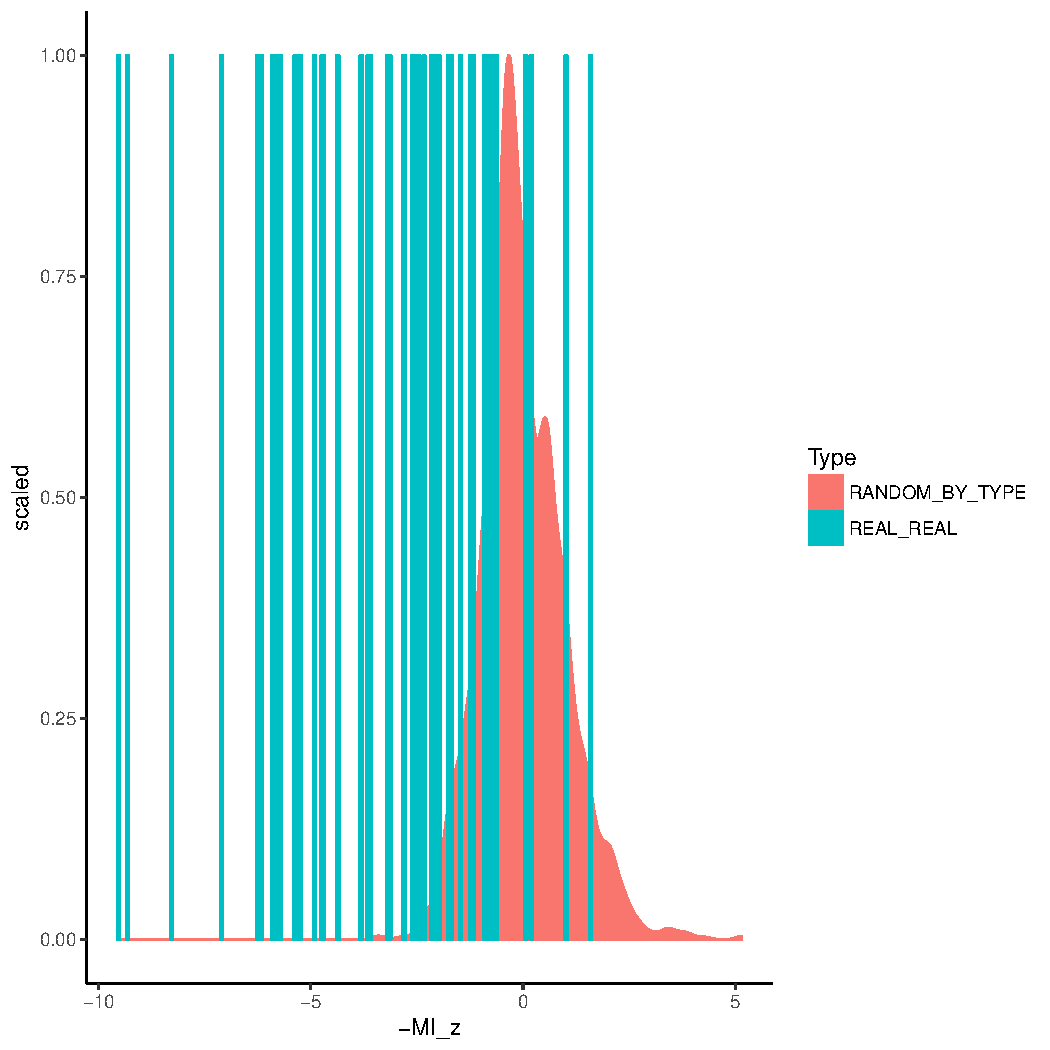
\includegraphics[width=0.5\textwidth]{../code/analysis/visualize_neural/figures/full-REAL-listener-surprisal-memory-HIST_z_byMem_onlyWordForms_boundedVocab.pdf}
%\captionof{figure}{Histogram}\label{fig:hist-real}
%\end{center}
%
%


\section{Formal Analysis and Proofs}

In this section, we prove Theorem 1.

\subsection{Mathematical Assumptions}

We first make explicit how we formalize language processing for proving the theorem.


\paragraph{Ingredient 1: Language as a Stationary Stochastic Process}
We represent language as a stochastic process of words $\dots w_{-2} w_{-1} w_0 w_{1} w_{2} \dots$, extending indefinitely both into the past and into the future.
The symbols $w_i$ belong to a common set, representing the words of the language.\footnote{Could also be phonemes, sentences, ..., any other kind of unit.}

%We model the sequence as a probabilistic sequence; that is, given a context $w_{<t}$, the next word is distributed according to a distribution $p(w_t|w_{<t})$.

The assumption of infinite length is for mathematical convenience and does not affect the substance of our results:
As we restrict our attention to the processing of individual sentences, which have finite length, we will actually not make use of long-range and infinite contexts.

We make the assumption that this process is \emph{stationary}.
Formally, this means that the conditional distribution $P(w_t|w_{<t})$ does not depend on $t$, it only depends on the (semi-infinite) context sequence $w_{<t}$.
Informally, this says that the process has no `internal clock', and that the statistical rules of the language do not change at the timescale we are interested in.
In reality, the statistical rules of language do change: They change as language changes over generations, and they also change between different situations -- e.g., depending on the interlocutor at a given point in time.
Given that we are interested in memory needs in the processing of \emph{individual sentences}, at a timescale of seconds or minutes, stationarity seems to be a reasonable assumption to make.


%
%
%
%\begin{figure}
%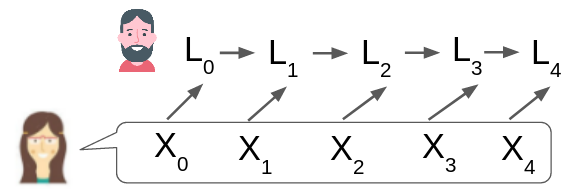
\includegraphics[width=0.45\textwidth]{figures/markov-condition.png}
%	\caption{Illustration of (\ref{eq:listener-markov}). As the utterance unfolds, the listener maintains a memory state. After receiving word $w_t$, the listener computes their new memory state $m_t$ based on the previous memory state $m_{t-1}$ and the new word $w_t$.}\label{fig:listener-markov}
%\end{figure}
%

\paragraph{Ingredient 2: Postulates about Processing}
The second ingredient consists of the three postulates described in the main paper.
%We now analyze memory from the perspective of the listener, who needs to maintain information about the past to predict the future.
%As the speaker's utterance unfolds, the listener maintains a memory state $m_t$.
There are no further assumptions about the memory architecture and the nature of its computations.
%We only make a basic assumption about the flow of information (Figure~\ref{fig:listener-markov}):
%At a given point in time, the listener's memory state $m_t$ is determined by the last word $w_t$, and the prior memory state $m_{t-1}$:
%\begin{equation}
%	m_t = M(m_{t-1}, w_t)
%\end{equation}
%As a consequence, $m_t$ contains no information about the process beyond what is contained in the last word observed $w_{t-1}$ and in the memory state before that word was observed $m_{t-1}$.
%%This is formalized as a statement about conditional probabilities:
%%\begin{equation}\label{eq:listener-markov}
%%p(m_1| (w_{t})_{t \in \mathbb{Z}}, m_0)   = p(m_1 | m_0, w_1)
%%\end{equation}
%%This says that $m_1$ contains no information about the utterances beyond what is contained in $m_0$ and $w_1$.	
%As a consequence, the listener has no knowledge of the speaker's state beyond the information provided in their prior communication.
%This is a simplification, as the listener could obtain information about the speaker from other sources, such as their common environment (weather, ...).
%\mhahn{For the study of memory in sentence processing, this seems fair. Discuss this more.}

%
%First, we assume that the listener's internal state cannot depend on the future beyond its dependency on the past.
%Formally: 
%\begin{equation}\label{eq:listener-markov-1}
%m_t \bot w_{>t} | w_{\leq t}
%\end{equation}
%This means that the listener has no access to the speaker's state beyond what the speaker has already uttered.
%
%Second, we assume that $m_t$ contains no information about the past beyond what is contained in $w_{t-1}$ and $m_{t-1}$:
%\begin{equation}\label{eq:listener-markov-2}
%m_t \bot w_{<t} | w_{t-1}, m_{t-1}
%\end{equation}
%This means that any information about the past in $m_t$ has to be contained in $m_{t-1}$ -- formalizing the idea that a listener can only remember aspects of the past by keeping them in memory, and that memories of the past cannot `spontaneously' form later in the future.

%The listener can trade off memory and future surprisal:
%A listener who chooses to store less memory will exerience higher surprisal in the future.
%A listener can achieve minimal surprisal -- that is, the lowest average surprisal that any model could achieve by predicting the future from the past -- if and only if $m_t$ contains all predictive information about the future that is contained in the past.

%We now describe the memory-surprisal tradeoff. will describe this tradeoff, and show that listener memory is linked to locality in a way similar to speaker memory.
%Consider a listener who uses $J$ bits of memory on average.
%What can we say about the listener's surprisal?

\subsection{Proof of the Theorem}

We restate the theorem:

\begin{thm}\label{prop:suboptimal}
	Let $T$ be any positive integer ($T \in \{1, 2, 3, ...\}$), and consider a listener using at most
	\begin{equation}\label{eq:memory}
		\sum_{t=1}^T t I_t
	\end{equation}
bits of memory on average.
Then this listener will incur surprisal at least
	$$H[w_t|w_{<t}] + \sum_{t > T} I_t$$
	on average.
\end{thm}



%We formalize a language as a stationary stochastic process $\dots w_{-2} w_{-1} w_0 w_{1} w_{2} \dots$, extending indefinitely both into the past and into the future.
%The symbols $w_i$ belong to a common set, representing the words of the language.\footnote{Could also be phonemes, sentences, ..., any other kind of unit.}
%We denote the listener's memory state at time $t$, after hearing $w_{<t} = ... w_{t-2} w_{t-1}$ by $m_t$.
%As described above, we assume
%\begin{equation}
%	m_t = M(m_{t-1}, w_{t-1})
%\end{equation}
%\footnote{Alternatively we could admit nondeterministic memory encodings, and require
%\begin{equation}\label{eq:listener-markov}
%	p(m_{t+1}| (w_{t'})_{t' \in \mathbb{Z}}, m_t)   = p(m_{t+1} | m_t, w_{t})
%\end{equation}
%that is, $m_{t+1}$ contains no information about the utterances beyond what is contained in $m_t$ and $w_{t}$.}
%As a consequence, the listener has no knowledge of the speaker's state beyond the information provided in their prior communication.


%The average number of bits required to encode this state is $\operatorname{H}[m_t]$, which by assumption is at most $\sum_{t=1}^T t I_t$.
%As the listener's predictions are made on the basis of her memory state, her average surprisal is at least $\operatorname{H}[w_t | m_t]$.
\begin{proof}
The difference between the listener's surprisal and optimal surprisal is $\operatorname{H}[w_t | m_t] - \operatorname{H}[w_t | w_{<t}]$.\footnote{A listener whose predictions are not optimal given $m_t$ can only incur even higher surprisal.}
By the assumption of stationarity, we can, for any positive integer $T$, rewrite this expression as
\begin{equation}\label{eq:byStation}
\operatorname{H}[w_t | m_t] - \operatorname{H}[w_t | w_{<t}] =  \frac{1}{T} \sum_{t'=1}^{T} \left(\operatorname{H}[w_{t'} | m_{t'}] - \operatorname{H}[w_{t'} | w_{<t'}]\right) 
\end{equation}
%NOTE the proof could be made simpler by taking $m_t$ to be a deterministic function of $x_t$, $m_{t-1}$, rather than talking about conditional independence
%
%We first show a lemma:
%
%\begin{lemma}
%For any positive integer $t$, the following inequality holds:
%\begin{equation}
%H[w_t | m_t] \geq H[w_t|w_{1 \dots t-1}, m_1]
%\end{equation}
%\end{lemma}
%
%\begin{proof}[Proof of the Lemma]
Because $m_t$ is determined by $(w_{1 \dots t-1}, m_1)$:
\begin{equation}
	m_t = M(m_{t-1}, w_{t-1}) = M(M(m_{t-2}, w_{t-2}), w_{t-1}) = M(M(M(m_{t-3}, w_{t-3}), w_{t-2}), w_{t-1}) = \dots
\end{equation}
the Data Processing inequality entails the following inequality for every positive integer $t$:
\begin{align}\label{eq:plugged}
\operatorname{H}[w_t | m_t]& \geq \operatorname{H}[w_t|w_{1\dots t-1}, m_1]
\end{align}
Plugging this inequality into Equation~\ref{eq:byStation} above:
\begin{align}\label{eq:plugged}
\operatorname{H}[w_t | m_t] - \operatorname{H}[w_t | w_{<t}]& \geq \frac{1}{T} \sum_{t=1}^T ( \operatorname{H}[w_t|w_{1\dots t-1}, m_1] - \operatorname{H}[w_t | w_{1\dots t-1}, w_{\leq 0}]  )    \\
& = \frac{1}{T} \left(\operatorname{H}[w_{1\dots T} | m_1] - \operatorname{H}[w_{1\dots T} | w_{\leq 0}]\right)  \\
& = \frac{1}{T} \left(I[w_{1\dots T}, w_{\leq 0}] - I[w_{1\dots T}, m_1]\right) 
\end{align}
The first term $I[w_{1\dots T}, w_{\leq 0}]$ can be rewritten in terms of $I_t$:
\begin{align}\label{eq:i-expanded}
I[w_{1\dots T}, w_{\leq 0}] &= \sum_{i=1}^T \sum_{j=-1}^{-\infty} I[w_i, w_j | w_{j+1}...w_{i-1}] = \sum_{t=1}^T t I_t + T \sum_{t > T} I_t
\end{align}
Therefore
\begin{align*}
\operatorname{H}[w_t | m_t] - \operatorname{H}[w_t | w_{<t}]& \geq \frac{1}{T} \left(\sum_{t=1}^T t I_t + T \sum_{t > T} I_t - I[w_{1\dots T}, m_1]\right) 
\end{align*}
$I[w_{1\dots T}|m_1]$ is at most $\operatorname{H}[m_1]$, which is at most $\sum_{t=1}^T t I_t$ by assumption. Thus, the expression above is bounded by
\begin{align*}
\operatorname{H}[w_t | m_t] - \operatorname{H}[w_t | w_{<t}]& \geq \frac{1}{T} \left(\sum_{t=1}^T t I_t + T \sum_{t > T} I_t - \sum_{t=1}^T t I_t\right) \\
&= \sum_{t > T} I_t
\end{align*}
Rearranging shows that the listener's surprisal is at least $\operatorname{H}[w_t|m_t] \geq \operatorname{H}[w_t | w_{<t}] + \sum_{t > T} I_t$, as claimed.
\end{proof}


%Justifylinear interpolation: The curve is convex, which is shown by `time-sharing': Use one code $\lambda$ fraction of times, and the other code $1-\lambda$ fraction of times.



\subsection{For nondeterministic encoding functions}

We have been assuming that $m_t$ is a deterministic function of $x_t$ and $m_{t-1}$.
Here, we show that this assumption can be relaxed to stochastic encoding functions.

We relax condition (X) to the following requirement, for all values of $m_1, (w_{t})_{t \in \mathbb{Z}}, m_0$:
\begin{equation}\label{eq:listener-markov-nondeterministic}
p(m_1| (w_{t})_{t \in \mathbb{Z}}, m_0)   = p(m_1 | m_0, w_1)
\end{equation}
This says that $m_1$ contains no information about the utterances beyond what is contained in $m_0$ and $w_1$.	

The one place in the proof where (X) plays a role is the proof of the inequality:
\begin{equation}
	H[w_t | m_t] \geq H[w_t|w_{1 \dots t-1}, m_1]
\end{equation}

We show that this inequality still holds under the relaxed condition (\ref{eq:listener-markov-nondeterministic}):
\begin{proof}
	By Bayes' Theorem
\begin{align*}
	p(w_t|m_0, m_1, w_{0\dots t-1}) &= \frac{p(m_1|m_0, w_{0\dots t})}{p(m_1|m_0, w_{0\dots t-1})} \cdot p(w_t|m_0, w_{0\dots t-1}) \\
 &= \frac{p(m_1|m_0, w_{0})}{p(m_1|m_0, w_{0})} \cdot p(w_t|m_0, w_{0\dots t-1}) \\
 &= p(w_t|m_0, w_{0\dots t-1}) \\
\end{align*}
	where the second equation follows from (\ref{eq:listener-markov-nondeterministic}).
So we have a Markov chain
\begin{equation}
(w_t) \rightarrow (m_0, w_{0 \dots t-1})   \rightarrow   (m_1, w_{1 \dots t-1})
\end{equation}
Thus, by the Data Processing Inequality,
\begin{equation}
H[w_t| w_{1 \dots t-1}, m_{1}] \geq H[w_t|w_{0 \dots t-1}, m_0]
\end{equation}
Finally, iteratively applying this reasoning, we conclude:
\begin{align*}
H[w_t | m_t] \geq H[w_t| w_{t-1}, m_{t-1}] \geq H[w_t| w_{t-2, t-1}, m_{t-2}] \geq ... \geq H[w_t|w_{1 \dots t-1}, m_1]
\end{align*}
\end{proof}


\subsection{Locality in a model with Memory Retrieval}

Here we show that our information-theoretic analysis is compatible with models placing the main bottleneck in the difficulty of retrieval \citep{mcelree2000sentence,lewis-activation-based-2005,nicenboim2018models,vasishth2019computational}.
We extend our model of memory in incremental prediction to capture key aspects of the models described by \citet{lewis-activation-based-2005,nicenboim2018models,vasishth2019computational}.

The ACT-R model of \cite{lewis-activation-based-2005} assumes a small working memory consisting of \emph{buffers} and a \emph{control state}, which together hold a small and fixed number of individual \emph{chunks}.
It also assumes a large short-term memory that contains an unbounded number of chunks.
This large memory store is accessed via \emph{cue-based retrieval}: a query is constructed based on the current state of the buffers and the control state; a chunk that matches this query is then selected from the memory storage and placed into one of the buffers.

\paragraph{Formal Model}
We extend our information-theoretic analysis by considering a model that maintains both a small working memory $m_t$ -- corresponding to the buffers and the control state -- and an unlimited short-term memory $s_t$.
Predictions are made based on working memory $m_t$, incurring surprisal $H[w_t|m_t]$.
When processing a word $x_t$, there is some amount of communication between $m_t$ and $s_t$, corresponding to retrieval operations.
We model this using a variable $r_t$ representing the information that is retrieved from $s_t$.
In our formalization, $r_t$ reflects the totality of all retrieval operations that are made during the processing of $x_{t-1}$; they happen after $x_{t-1}$ has been observed but before $x_t$ has.

The working memory state is determined not just by the input $x_t$ and the previous working memory state $m_{t-1}$, but also by the retrieved information:
\begin{equation}
	m_t = f(x_t, m_{t-1}, r_t) 
\end{equation}
The retrieval operation is jointly determined by working memory, short-term memory, and the previous word:
\begin{equation}\label{eq:rt}
	r_t = g(x_{t-1}, m_{t-1}, s_{t-1}) 
\end{equation}
Finally, the short-term memory can incorporate any -- possibly all -- information from the last word and the working memory:
\begin{equation}
	s_t = h(x_{t-1}, m_{t-1}, s_{t-1}) 
\end{equation}
While $s_t$ is unconstrained, there are constraints on the capacity of working memory $\operatorname{H}[m_t]$ and the amount of retrieved information $\operatorname{H}[r_t]$.
Placing a bound on $\operatorname{H}[m_t]$ reflects the fact that the buffers can only hold a small and fixed number of chunks \citep{lewis-activation-based-2005}.


\paragraph{Cost of Retrieval}
%In ACT-R, each retrieval operation is initiated through a query constructed based on the current state of the buffers; it returns a chunk from short-term memory that is then placed into a buffer.
%Equation~\ref{eq:rt} reflects that these retrieved chunks are determined by working memory and short-term memory.
In the model of \cite{lewis-activation-based-2005}, the time it takes to process a word is determined primarily by the time spent retrieving chunks, which is determined by the number of retrieval operations and the time it takes to complete each retrieval operation.
If the information content of each chunk is bounded, then a bound on $H[r_t]$ corresponds to a bound on the number of retrieval operations.

In the model of \cite{lewis-activation-based-2005}, a retrieval operation takes longer if more chunks are similar to the retrieval cue, whereas, in the direct-access model \citep{mcelree2000sentence,nicenboim2018models,vasishth2019computational}, retrieval operations take a constant amount of time.
There is no direct counterpart to differences in retrieval times and similarity-based inhibition as in the activation-based model in our formalization.
Our formalization thus more closely matches the direct-access model, though it might be possible to incorporate aspects of the activation-based model in our formalization.

\paragraph{Role of Surprisal}
The ACT-R model of \cite{lewis-activation-based-2005} does not have an explicit surprisal cost.
Instead, surprisal effects are interpreted as arising because, in less constraining contexts, the parser is more likely to make decisions that then turn out to be incorrect, leading to additional correcting steps.
%We see this as an algorithmic-level implementation of the justification for surprisal theory provided by \citet{levy2008expectation}:
We view this as an algorithmic-level implementation of a surprisal cost $H[x_t|m_{t-1}]$:
If the word $x_t$ is unexpected given the current state of the working memory -- i.e., buffers and control states -- then their current state must provide insufficient information to constrain the actual syntactic state of the sentence, meaning that the parsing steps made to integrate $x_t$ are likely to include more backtracking and correction steps.
Thus, we argue that cue-based retrieval models predict that the surprisal $- \log P(x_t|m_{t-1})$ will be part of the cost of processing word $x_t$.


%This is instantiated by ACT-R.
%We can explicitly explain how this covers the McElree ideas and the Lewis and Vasishth ACT-R model.
%This model has two bottlenecks:
%The working memory capacity, which we model as $H[m_t]$, and the amount of information that is added through retrieval, modeled as $H[r_t|m_t]$.
%Bounding retrieval = bounding the precision and/or content of retrieved items. Explain more how this relates to McElree and ACT-R.
%In ACT-R, each retrieval operation takes time. If each chunk has a bounded amount of information, then this corresponds to a bottleneck in $H[r_t|m_t]$

\paragraph{Theoretical Result}
We now show an extension of our theoretical result in the setting of the retrieval-based model described above.

\begin{thm}
Let $0 < S \leq T$ be positive integers such that the average working memory cost $\operatorname{H}[m_t]$ is bounded as
	\begin{equation}
		\operatorname{H}[m_t] \leq \sum_{t=1}^T t I_t
	\end{equation}
	and the average amount of retrieved information is bounded as
	\begin{equation}
		\operatorname{H}[r_t] \leq \sum_{t=T+1}^S I_t
	\end{equation} %(per word).
	Then the surprisal cost is lower-bounded as
	\begin{equation}
		\operatorname{H}[w_t|m_t] \geq \operatorname{H}[w_t|x_{<t}] + \sum_{t>S} I_t
	\end{equation}
\end{thm}

\begin{proof}
The proof is a generalization of the proof above.
	For any positive integer $t$, $m_t$ is determined by $w_{1\dots t}, m_0, r_0, \dots, r_t$.
	Therefore, the Data Processing Inequality entails:
	\begin{equation}
		\operatorname{H}[w_t|m_t] \geq \operatorname{H}[w_t|w_{1\dots t}, m_0, r_0, \dots, r_t]
	\end{equation}
	As in~(\ref{eq:plugged}), this leads to
\begin{align}
\operatorname{H}[w_t | m_t] - \operatorname{H}[w_t | w_{<t}]& \geq \frac{1}{T} \sum_{t=1}^T ( \operatorname{H}[w_t|w_{1\dots t}, m_0, r_0, \dots, r_t] - \operatorname{H}[w_t | w_{1\dots t-1}, w_{\leq 0}]  )    \\
& \geq \frac{1}{T} \left(\operatorname{H}[w_{1\dots T} | m_0, r_0, \dots, r_T] - \operatorname{H}[w_{1\dots T} | w_{\leq 0}]\right)  \\
	& = \frac{1}{T} \left(I[w_{1\dots T}, w_{\leq 0}] - I[w_{1\dots T}, (m_0, r_0, \dots, r_T)]\right) 
\end{align}
	Now, using the calculation from (\ref{eq:i-expanded}), this can be rewritten as:
	\begin{align*}
\operatorname{H}[w_t | m_t] - \operatorname{H}[w_t | w_{<t}]= & \frac{1}{T}\left(\sum_{t=1}^T t I_t + T \sum_{t>T} I_t - I[X_1\dots X_T, (M_0, R_1, ..., R_T)]\right) \\
		= & \frac{1}{T}\left(\sum_{t=1}^T t I_t + T \sum_{t>T} I_t - I[X_{1\dots T}, M_0] - \sum_{t=1}^T I[X_{1\dots T}, R_t|M_0, r_{1\dots t-1}]\right) \\
	\end{align*}
	Due to the inequalities $I[X_{1\dots T}, M_0] \leq \operatorname{H}[M_0]$ and $\operatorname{I}[X_{1\dots T}, R_t|M_0, r_{1\dots t-1}] \leq \operatorname{H}[R_t]$, this can be bounded as
	\begin{align}
\operatorname{H}[w_t | m_t] - \operatorname{H}[w_t | w_{<t}]		\geq & \frac{1}{T}\left(\sum_{t=1}^T t I_t  + T \sum_{t>T} I_t-H[M_0] - \sum_{t=1}^T H[R_t]\right) \\
	\end{align}
	Finally, this reduces as
	\begin{align}
	\operatorname{H}[w_t | m_t] - \operatorname{H}[w_t | w_{<t}]		\geq &  \frac{1}{T}(T \sum_{t>T} I_t - T\cdot H[R_t]) \\
	= & \sum_{t>T} I_t- H[R_t]  \\
		\geq & \sum_{t>T} I_t - \sum_{t=T+1}^S I_t \\
		= &  \sum_{t>S} I_t
\end{align}

\end{proof}

\paragraph{Information Locality}
We now show that this result predicts information locality provided that retrieving information is more expensive than keeping the same amount of information in working memory.
For this, we formalize the problem of finding an optimal memory strategy as a multi-objective optimization, aiming to minimize
\begin{equation}
	\lambda_1 H[m_t] + \lambda_2 H[r_t]
\end{equation}
to achieve a given surprisal level, for some setting of $\lambda_1, \lambda_2 > 0$ describing the relative cost of storage and retrieval.
What is the optimal division of labor between keeping information in working memory and recovering it through retrieval?
The problem
\begin{equation}\label{eq:multi-obj-t}
	\min_{T} \lambda_1 \sum_{t=1}^T t I_t + \lambda_2 \sum_{t=T+1}^S I_t
\end{equation}
has solution $T \approx \frac{\lambda_2}{\lambda_1}$. %\footnote{Can do simple proof using the continuous-$T$-version.}
This means that, as long as retrievals are more expensive than keeping the same amount of information in working memory (i.e., $\lambda_2 > \lambda_1$), the optimal strategy stores information from the last $T > 1$ words in working memory.
Due to the factor $t$ inside $\sum_{t=1}^T t I_t$, the bound~(\ref{eq:multi-obj-t}) will be reduced when $I_t$ decays faster, i.e., there is strong information locality.

The assumption that retrieving information is more difficult than storing it is reasonable for cue-based retrieval models, as retrieval suffers from similarity-based interference effects due to the unstructured nature of the storage~\citep{lewis-activation-based-2005}.
A model that maintains no information in its working memory, i.e. $H[m_t]=0$, would correspond to a cue-based retrieval model that stores nothing in its buffers and control states, and relies entirely on retrieval to access past information.
Given the nature of representations assumed in models~\citep{lewis-activation-based-2005}, such a model would seem to be severely restricted in its ability to parse language.

%If $\frac{\lambda_2}{\lambda_1} \rightarrow \infty$ (retrievals get more expensive), recover previous model.
%If $\frac{\lambda_2}{\lambda_1} \rightarrow 0$ (retrievals get cheaper), locality effect gets weaker, and disappears in the limit\footnote{(Of course, even in this limit, there might be additional factors that may still favor locality in a specific implementation of memory -- e.g., in ACT-R, decay and interference are less problematic if there is locality.)}




\subsection{Results for Language Production}

Here we show results linking memory and locality in production.
We show that results similar to our main theorem hold for the tradeoff between a speaker's memory and the accuracy with which they match the distribution of the language.



\paragraph{Speaker aims to match language distribution}
First, we consider a setting in which a speaker produces sentences with bounded memory, and analyze the deviation of the produced distribution from the actual distribution of the language.

We consider a speaker who maintains memory representations and incrementally produces based on these representations:
\begin{equation}
	p_{speaker}(x_t|X_{<t}) = p(x_t|m_t) \\
\end{equation}
We show a tradeoff between the memory capacity $\operatorname{H}[m_t]$ and the KL-divergence between the actual language statistics and the speaker's production distribution:
\begin{equation}
D_{KL}(P_{language}||P_{produced})  := \E_{X_{<t}} \sum_{x_t} p(x_t|X_{<t}) \log \frac{p(x_t|X_{<t})}{p_{speaker}(x_t|X_{<t})} \\
\end{equation}
\begin{thm}
If a speaker maintains memory
	\begin{equation}
		\operatorname{H}[m_t] \leq \sum_{i=1}^T tI_t
	\end{equation}
	then 
\begin{equation}
	D_{KL}(P_{language}||P_{produced}) \geq \sum_{t=T+1}^\infty I_t
\end{equation}
\end{thm}

While this bound only considers the production of a single word, it immediately entails a bound on the production accuracy for sequences:
\begin{equation}
	D_{KL}(P_{language}(X_1\dots X_t|X_{\leq 0})||P_{produced}(X_1\dots X_t|X_{\leq 0}))  = t \cdot D_{KL}(P_{language}(X_1|X_{\leq 0})||P_{produced}(X_1|X_{\leq 0}))
\end{equation}



\begin{proof}
First note
\begin{align}
D_{KL}(P_{language}||P_{produced}) & = \E_{X_{<t}} \sum_{x_t} p(x_t|X_{<t}) \log \frac{p(x_t|X_{<t})}{p_{speaker}(x_t|X_{<t})} \\
& = \E_{X_{<t}} \sum_{x_t} p(x_t|X_{<t}) \log \frac{p(x_t|X_{<t})}{p(x_t|M(X_{<t}))} \\
& = \E_{X_{<t}} \sum_{x_t} p(x_t|X_{<t}) \log p(x_t|X_{<t}) - \E_{X_{<t}} \sum_{x_t} p(x_t|X_{<t}) \log p(x_t|M(X_{<t})) \\
	& = \E_{X_{<t}} \sum_{x_t} p(x_t|X_{<t}) \log p(x_t|X_{<t}) + S_M(x_t|X_{<t})
\end{align}
In the last line, the first term is a constant independent of $M$.

Then the proof for the listener case transfers to this setting.
\end{proof}

TODO limitations of this as a model of production




\paragraph{Speaker aims to match, conditional on goal}
The first setting does not account for the fact that language is produced aiming for some communicative goal.
We therefore now assume that the speaker has a communicative goal $G$ in mind.
This goal $G$ stays constant during production process for a sentence, and we count how much memory is needed in addition to the goal $G$.
We assume that there is a distribution of sentences expressing goals $G$:
\begin{equation}
	P(sentence|G)
\end{equation}
and assume that the speaker aims to match this distribution
\begin{equation}
\mathbb{E}_G[D_{KL}((language|G)||(produced|G))]
\end{equation}
We can analyze this model by adding conditioning w.r.t. $G$ throughout the analysis of the previous case.
Specifically, we need
\begin{equation}
I_t^G := I[X_t, X_0|X_1, \dots, X_{t-1}, G]
\end{equation}

Take $I_t$ conditioned on $G$: only count statistical dependencies to the degree that they are not redundant with the goal


\begin{thm}
If a speaker maintains memory
	\begin{equation}
		\operatorname{H}[m_t] \leq \sum_{i=1}^T tI_t^G
	\end{equation}
	then 
\begin{equation}
\E_G	D_{KL}(P_{language}(\cdot|G)||P_{produced}(\cdot|G)) \geq \sum_{t=T+1}^\infty I_t^G
\end{equation}
\end{thm}

\begin{proof}
This is entirely analogous to the previous proof.
\end{proof}


are there conditions under which this is close to $I_t$?

\paragraph{Pragmatic Speaker}

would need an assumption on the density of goals in the space of sequences.


Note 
\begin{equation}
	D_{KL}(P_{language}(x_{1\dots t})||P_{produced}(x_{1\dots t}))  := \sum_{x_{1\dots t}} p(x_t|X_{1\dots t}) \log \frac{p(x_t|X_{1\dots t})}{p_{speaker}(x_t|X_{1\dots t})} \geq t D_KL(x_t||...)
\end{equation}

$H[G|Produced] - H[G|Language]$



\section{Proof of Left-Right Invariance}

Here we show that the bound provided by our theorem is invariant under reversal of the process.
That is: Given a process $(X_t)_{t \in \mathbb{Z}}$, we define its reverse process $(Y_t)_{t \in \mathbb{Z}}$ by $Y_t := X_t$.
We claim that the theorem provides the same bounds for the memory-surprisal tradeoff curves.
To prove this, we note:
\begin{equation}
	I[X_t, X_0|X_{1\dots t-1}] = I[Y_{-t}, Y_0|Y_{1-t\dots -1}] = I[Y_0, Y_t|Y_{1\dots t-1}] = I[Y_t, Y_0|Y_{1\dots t-1}]
\end{equation}
The first step follows from the definition of $Y$. The second step follows from the fact that $X_t$, and thus also $Y_t$, is stationary, and thus adding $t$ to each index in the expression does not change the resulting value. The third step uses the fact that mutual information is symmetric.


\section{Example where window model is not optimal}

Here we provide an example of a stochastic process where a window-based memory encoding is not optimal, but the bound provided by our theorem still holds.

Let $k$ be some positive integer.
Consider a process
$x_{t+1} = (v_{t+1}, w_{t+1}, y_{t+1}, z_{t+1})$
where
\begin{enumerate}
	\item The first two components consist of fresh random bits. Formally, $v_{t+1}$ is an independent draw from $Bernoulli(0.5)$, independent from all preceding observations $x_{\leq t}$.
		Second, let $w_{t+1}$ consist of $2k$ many such independent random bits (so that $H[w_{t+1}] = 2k$)
	\item The third component \emph{deterministically} copies the first bit from $2k$ steps earlier. Formally, $y_{t+1}$ is equal to the first component of $x_{t-2k+1}$
	\item The fourth component \emph{stochastically} copies the second part (consisting of $2k$ random bits) from one step earlier. Formally, each component $z_{t+1}^{(i)}$ is determined as follows: First take a sample $u_{t+1}^{(i)}$ from $Bernoulli(\frac{1}{4k})$, independent from all preceding observations.
		If $u_{z+1}^{(i)}=1$, set $z_{t+1}^{(i)}$ to be equal to the second component of $w_{t}^{(i)}$.
		Otherwise, let $z_{t+1}^{(i)}$ be a fresh draw from $Bernoulli(0.5)$.
\end{enumerate}

Predicting observations optimally requires taking into account observations from the $2k$ last time steps.

We show that, when approximately predicting with low memory capacities, a window-based approach does \emph{not} in general achieve an optimal memory-surprisal tradeoff.

Consider a model that predicts $x_{t+1}$ from only the last observation $x_t$, i.e., uses a window of length one.
The only relevant piece of information in this past observation is $w_t$, which stochastically influences $z_{t+1}$.
Storing this costs $2k$ bit of memory as $w_t$ consists of $2k$ draws from $Bernoulli(0.5)$.
How much does it reduce the surprisal of $x_{t+1}$?
Due to the stochastic nature of $z_{t+1}$, it reduces the surprisal only by about $I[x_{t+1}, w_t] = I[z_{t+1}, w_t] < 2k \cdot \frac{1}{2k} = 1$, i.e., surprisal reduction is strictly less than one bit.
\footnote{We can evaluate $I[z_{t+1}, w_t]$ as follows. Set $l = k/4$. Write $z, w$ for any of the $2k$ components of $z_{t+1}, w_t$, respectively. First, calculate $p(z = 1|w=1) = 1/l + (1-1/l) \frac{1}{2} = 1/(2l) + 1/2 = \frac{1+l}{2l}$ and $p(z = 0|w=1) = (1-1/l) \frac{1}{2} = 1/2 - 1/2l = \frac{l-1}{2l}$.
Then $I[Z, W] = D_{KL}(p(z|w=1)||p(z)) = \frac{1+l}{2l} \log \frac{\frac{1+l}{2l}}{1/2} + \frac{l-1}{2l} \log \frac{\frac{l-1}{2l}}{1/2}  = \frac{1+l}{2l} \log \frac{1+l}{l} + \frac{l-1}{2l} \log \frac{l-1}{l}  \leq \frac{1+l}{l} \log \frac{1+l}{l} =  (1+1/l) \log (1+1/l)  \leq  (1+1/l) (1/l) = 1/l + 1/l^2 < 2/l = \frac{1}{2k}.$
%Then $H[Z|w=1] = - \frac{1+k}{2k} \log \frac{1+k}{2k} - \frac{k-1}{2k} \log \frac{k-1}{2k}  = - (1/2 + 1/2k) \log \frac{1+k}{2k} - (1/2 - 1/2k) \log \frac{k-1}{2k}$ %= - \frac{1+k}{2k} \log (1+k) - \frac{k-1}{2k} \log (k-1) + \log 2k = - \frac{1+k}{2k} \log (1+k) - \frac{k-1}{2k} \log (k-1) + \log 2k$.
}

We show that there is an alternative model that strictly improves on this window-based model:
Consider a memory encoding model that encodes each of $v_{t-2k+1}, \dots, v_{t}$, which costs $2k$ bits of memory -- as the window-based model did.
Since $y_{t+1} = v_{t-2k+1}$, this model achieves a surprisal reduction of $H[v_{t-2k+1}] = 1$ bit, strictly more than the window-based model.


This result does not contradict our theorem because the theorem only provides \emph{bounds} across models, which are not necessarily achieved by a given window-based model.
In fact, for the process described here, no memory encoding function $M$ can exactly achieve the theoretical bound described by the theorem.

\section{Corpus Size per Language}

\begin{center}
\begin{longtable}{l|ll||l|llllllllllllll}
	Language & Training & Held-Out & 	Language & Training & Held-Out\\ \hline
Afrikaans  &  1,315  &  194  &  Indonesian  &  4,477  &  559  \\
Amharic  &  974  &  100  &  Italian  &  17,427  &  1,070  \\
Arabic  &  21,864  &  2,895  &  Japanese  &  7,164  &  511  \\
Armenian  &  514  &  50  &  Kazakh  &  947  &  100  \\
Bambara  &  926  &  100  &  Korean  &  27,410  &  3,016  \\
Basque  &  5,396  &  1,798  &  Kurmanji  &  634  &  100  \\
Breton  &  788  &  100  &  Latvian  &  4,124  &  989  \\
Bulgarian  &  8,907  &  1,115  &  Maltese  &  1,123  &  433  \\
Buryat  &  808  &  100  &  Naija  &  848  &  100  \\
Cantonese  &  550  &  100  &  North Sami  &  2,257  &  865  \\
Catalan  &  13,123  &  1,709  &  Norwegian  &  29,870  &  4,639  \\
Chinese  &  3,997  &  500  &  Persian  &  4,798  &  599  \\
Croatian  &  7,689  &  600  &  Polish  &  6,100  &  1,027  \\
Czech  &  102,993  &  11,311  &  Portuguese  &  17,995  &  1,770  \\
Danish  &  4,383  &  564  &  Romanian  &  8,664  &  752  \\
Dutch  &  18,310  &  1,518  &  Russian  &  52,664  &  7,163  \\
English  &  17,062  &  3,070  &  Serbian  &  2,935  &  465  \\
Erzya  &  1,450  &  100  &  Slovak  &  8,483  &  1,060  \\
Estonian  &  6,959  &  855  &  Slovenian  &  7,532  &  1,817  \\
Faroese  &  1,108  &  100  &  Spanish  &  28,492  &  3,054  \\
Finnish  &  27,198  &  3,239  &  Swedish  &  7,041  &  1,416  \\
French  &  32,347  &  3,232  &  Thai  &  900  &  100  \\
German  &  13,814  &  799  &  Turkish  &  3,685  &  975  \\
Greek  &  1,662  &  403  &  Ukrainian  &  4,506  &  577  \\
Hebrew  &  5,241  &  484  &  Urdu  &  4,043  &  552  \\
Hindi  &  13,304  &  1,659  &  Uyghur  &  1,656  &  900  \\
Hungarian  &  910  &  441  &  Vietnamese  &  1,400  &  800  \\

\end{longtable}
	\captionof{table}{Languages, with the number of training and held-out sentences available.}\label{tab:corpora}
\end{center}

\section{Samples Drawn per Language}

\begin{center}
\begin{longtable}{l|ll||l|llllllllllllll}
	Language & Base. & Real & Language & Base. & Real \\ \hline
Afrikaans  &  13  &  10  &  Indonesian  &  11  &  11  \\
Amharic  &  137  &  10  &  Italian  &  10  &  10  \\
Arabic  &  11  &  10  &  Japanese  &  25  &  15  \\
Armenian  &  140  &  76  &  Kazakh  &  11  &  10  \\
Bambara  &  25  &  29  &  Korean  &  11  &  10  \\
Basque  &  15  &  10  &  Kurmanji  &  338  &  61  \\
Breton  &  35  &  14  &  Latvian  &  308  &  178  \\
Bulgarian  &  14  &  10  &  Maltese  &  30  &  24  \\
Buryat  &  26  &  18  &  Naija  &  214  &  10  \\
Cantonese  &  306  &  32  &  North Sami  &  335  &  194  \\
Catalan  &  11  &  10  &  Norwegian  &  12  &  10  \\
Chinese  &  21  &  10  &  Persian  &  25  &  12  \\
Croatian  &  30  &  17  &  Polish  &  309  &  35  \\
Czech  &  18  &  10  &  Portuguese  &  15  &  55  \\
Danish  &  33  &  17  &  Romanian  &  10  &  10  \\
Dutch  &  27  &  10  &  Russian  &  20  &  10  \\
English  &  13  &  11  &  Serbian  &  26  &  11  \\
Erzya  &  846  &  167  &  Slovak  &  303  &  27  \\
Estonian  &  347  &  101  &  Slovenian  &  297  &  80  \\
Faroese  &  27  &  13  &  Spanish  &  14  &  10  \\
Finnish  &  83  &  16  &  Swedish  &  31  &  14  \\
French  &  14  &  11  &  Thai  &  45  &  19  \\
German  &  19  &  13  &  Turkish  &  13  &  10  \\
Greek  &  16  &  10  &  Ukrainian  &  28  &  18  \\
Hebrew  &  11  &  10  &  Urdu  &  17  &  10  \\
Hindi  &  11  &  10  &  Uyghur  &  326  &  175  \\
Hungarian  &  220  &  109  &  Vietnamese  &  303  &  12  \\

\end{longtable}
	\captionof{figure}{Samples drawn per language according to the precision-dependent stopping criterion.}\label{tab:samples}
\end{center}



\begin{center}
\begin{longtable}{l|lll||l|lllllllllllllll}
	Language & Mean & Lower & Upper & Language & Mean & Lower & Upper \\ \hline
Afrikaans  &  1.0  &  1.0  &  1.0  &  Indonesian  &  1.0  &  1.0  &  1.0  \\
Amharic  &  1.0  &  1.0  &  1.0  &  Italian  &  1.0  &  1.0  &  1.0  \\
Arabic  &  1.0  &  1.0  &  1.0  &  Japanese  &  1.0  &  1.0  &  1.0  \\
Armenian  &  0.92  &  0.87  &  0.97  &  Kazakh  &  1.0  &  1.0  &  1.0  \\
Bambara  &  1.0  &  1.0  &  1.0  &  Korean  &  1.0  &  1.0  &  1.0  \\
Basque  &  1.0  &  1.0  &  1.0  &  Kurmanji  &  0.93  &  0.88  &  0.98  \\
Breton  &  1.0  &  1.0  &  1.0  &  Latvian  &  0.49  &  0.4  &  0.57  \\
Bulgarian  &  1.0  &  1.0  &  1.0  &  Maltese  &  1.0  &  1.0  &  1.0  \\
Buryat  &  1.0  &  1.0  &  1.0  &  Naija  &  1.0  &  0.99  &  1.0  \\
Cantonese  &  0.96  &  0.86  &  1.0  &  North Sami  &  0.37  &  0.3  &  0.44  \\
Catalan  &  1.0  &  1.0  &  1.0  &  Norwegian  &  1.0  &  1.0  &  1.0  \\
Chinese  &  1.0  &  1.0  &  1.0  &  Persian  &  1.0  &  1.0  &  1.0  \\
Croatian  &  1.0  &  1.0  &  1.0  &  Polish  &  0.1  &  0.04  &  0.17  \\
Czech  &  1.0  &  1.0  &  1.0  &  Portuguese  &  1.0  &  1.0  &  1.0  \\
Danish  &  1.0  &  1.0  &  1.0  &  Romanian  &  1.0  &  1.0  &  1.0  \\
Dutch  &  1.0  &  1.0  &  1.0  &  Russian  &  1.0  &  1.0  &  1.0  \\
English  &  1.0  &  1.0  &  1.0  &  Serbian  &  1.0  &  1.0  &  1.0  \\
Erzya  &  0.99  &  0.98  &  1.0  &  Slovak  &  0.07  &  0.03  &  0.12  \\
Estonian  &  0.8  &  0.72  &  0.86  &  Slovenian  &  0.82  &  0.77  &  0.88  \\
Faroese  &  1.0  &  1.0  &  1.0  &  Spanish  &  1.0  &  1.0  &  1.0  \\
Finnish  &  1.0  &  1.0  &  1.0  &  Swedish  &  1.0  &  1.0  &  1.0  \\
French  &  1.0  &  1.0  &  1.0  &  Thai  &  1.0  &  1.0  &  1.0  \\
German  &  1.0  &  0.91  &  1.0  &  Turkish  &  1.0  &  1.0  &  1.0  \\
Greek  &  1.0  &  1.0  &  1.0  &  Ukrainian  &  1.0  &  1.0  &  1.0  \\
Hebrew  &  1.0  &  1.0  &  1.0  &  Urdu  &  1.0  &  1.0  &  1.0  \\
Hindi  &  1.0  &  1.0  &  1.0  &  Uyghur  &  0.65  &  0.57  &  0.73  \\
Hungarian  &  0.87  &  0.8  &  0.93  &  Vietnamese  &  1.0  &  0.98  &  1.0  \\

\end{longtable}
	\captionof{figure}{Bootstrapped estimates for $G$.}\label{tab:boot-g}
\end{center}


\section{Detailed Results per Language}

\subsection{Median Surprisal per Memory Budget}

\begin{center}
\begin{longtable}{ccccccccccccccclll}
Afrikaans & Amharic & Arabic & Armenian
 \\ 
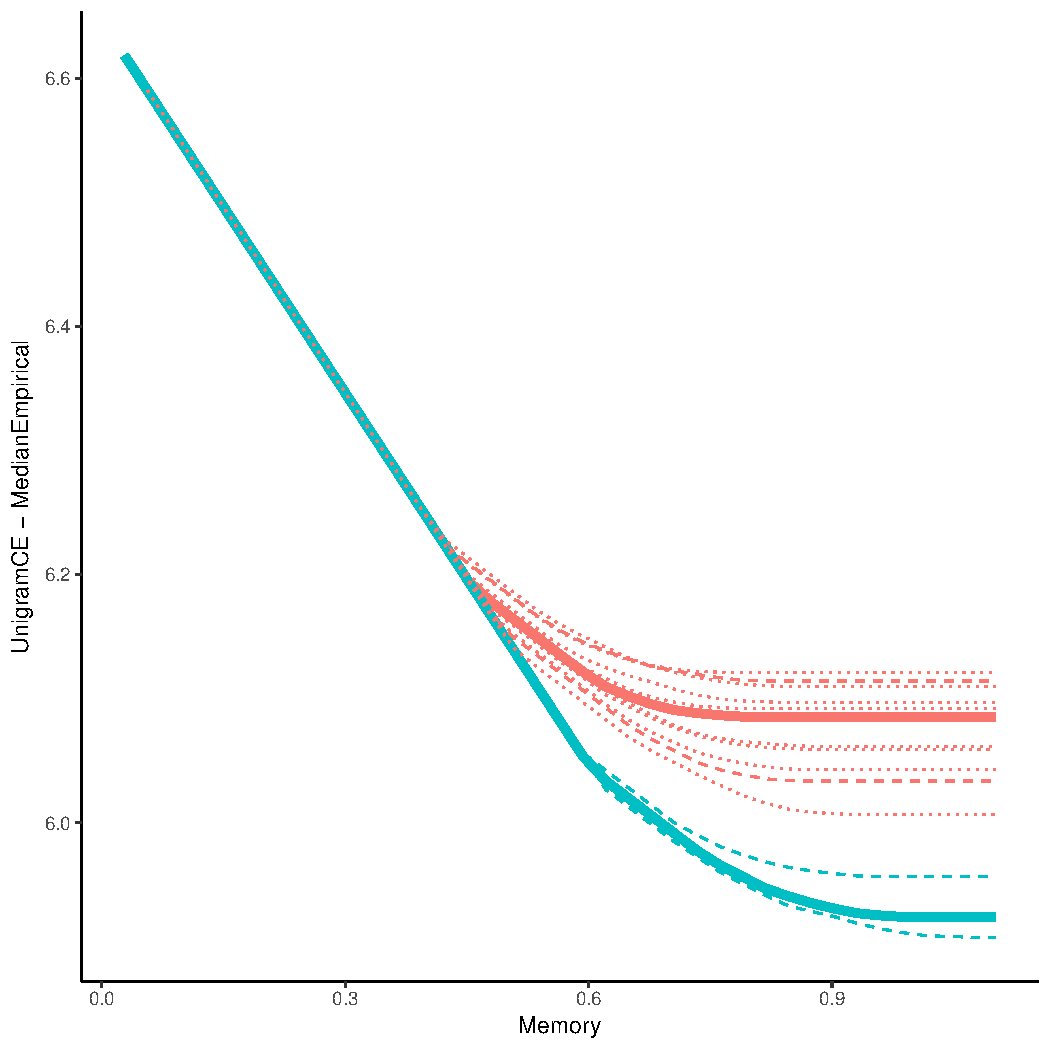
\includegraphics[width=0.25\textwidth]{neural/figures/Afrikaans-listener-surprisal-memory-MEDIANS_QUANTILES_onlyWordForms_boundedVocab_REAL.pdf} & 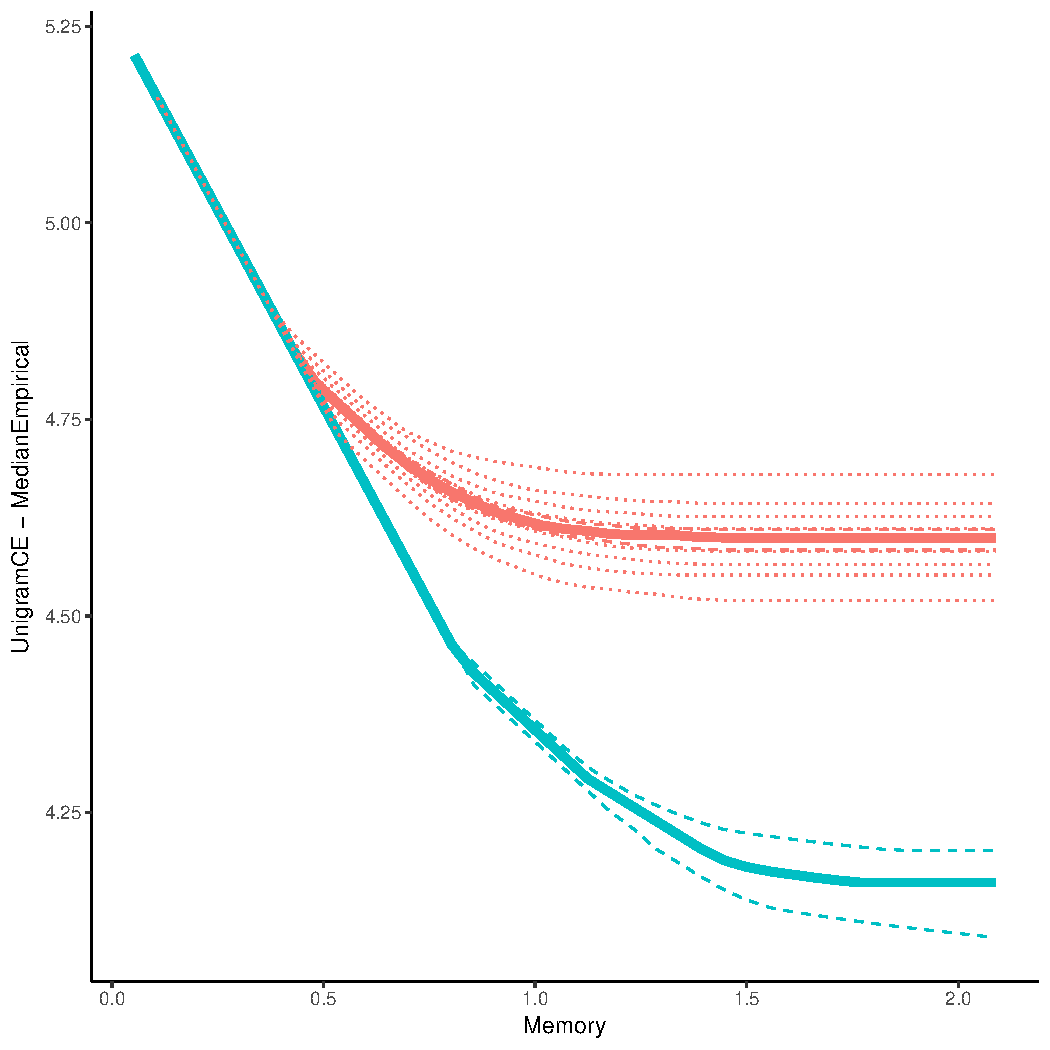
\includegraphics[width=0.25\textwidth]{neural/figures/Amharic-Adap-listener-surprisal-memory-MEDIANS_QUANTILES_onlyWordForms_boundedVocab_REAL.pdf} & 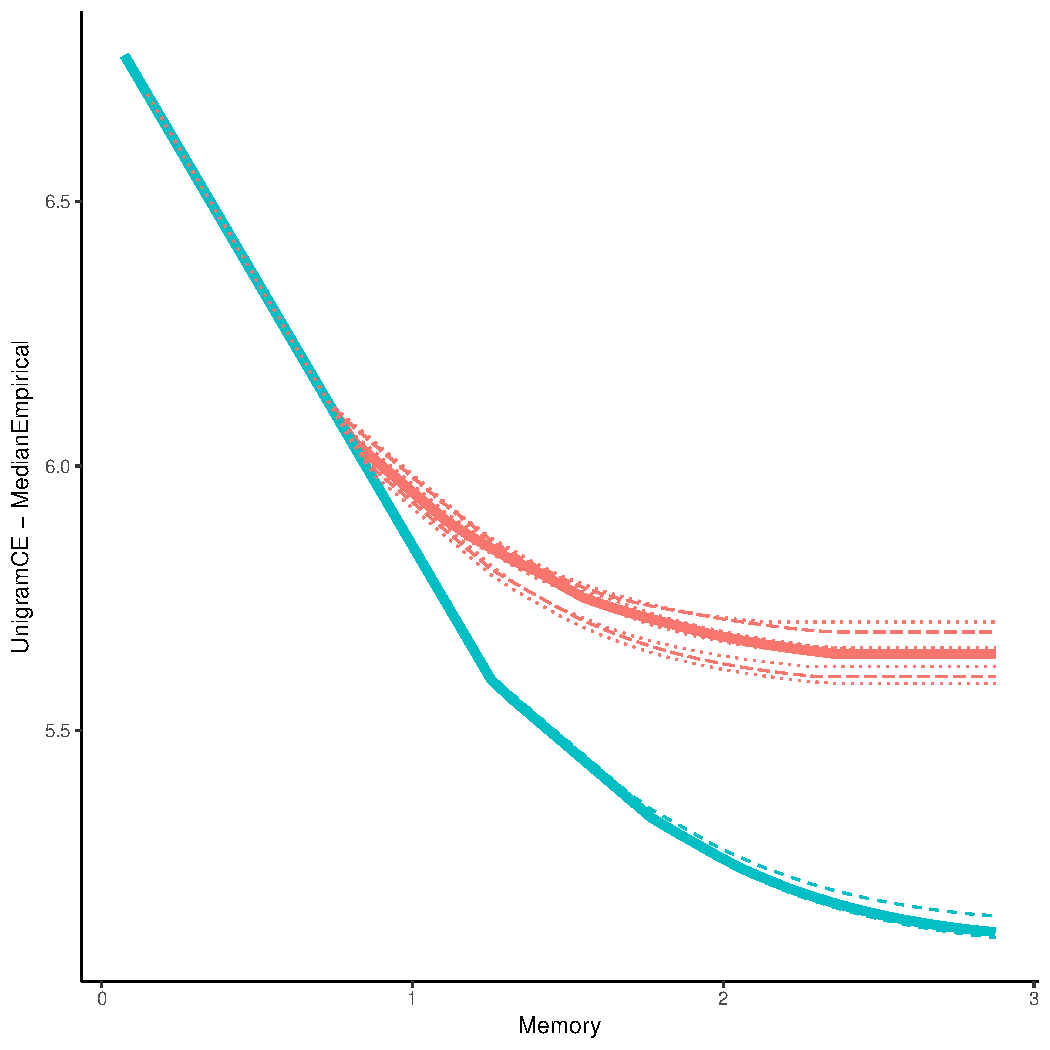
\includegraphics[width=0.25\textwidth]{neural/figures/Arabic-listener-surprisal-memory-MEDIANS_QUANTILES_onlyWordForms_boundedVocab_REAL.pdf} & 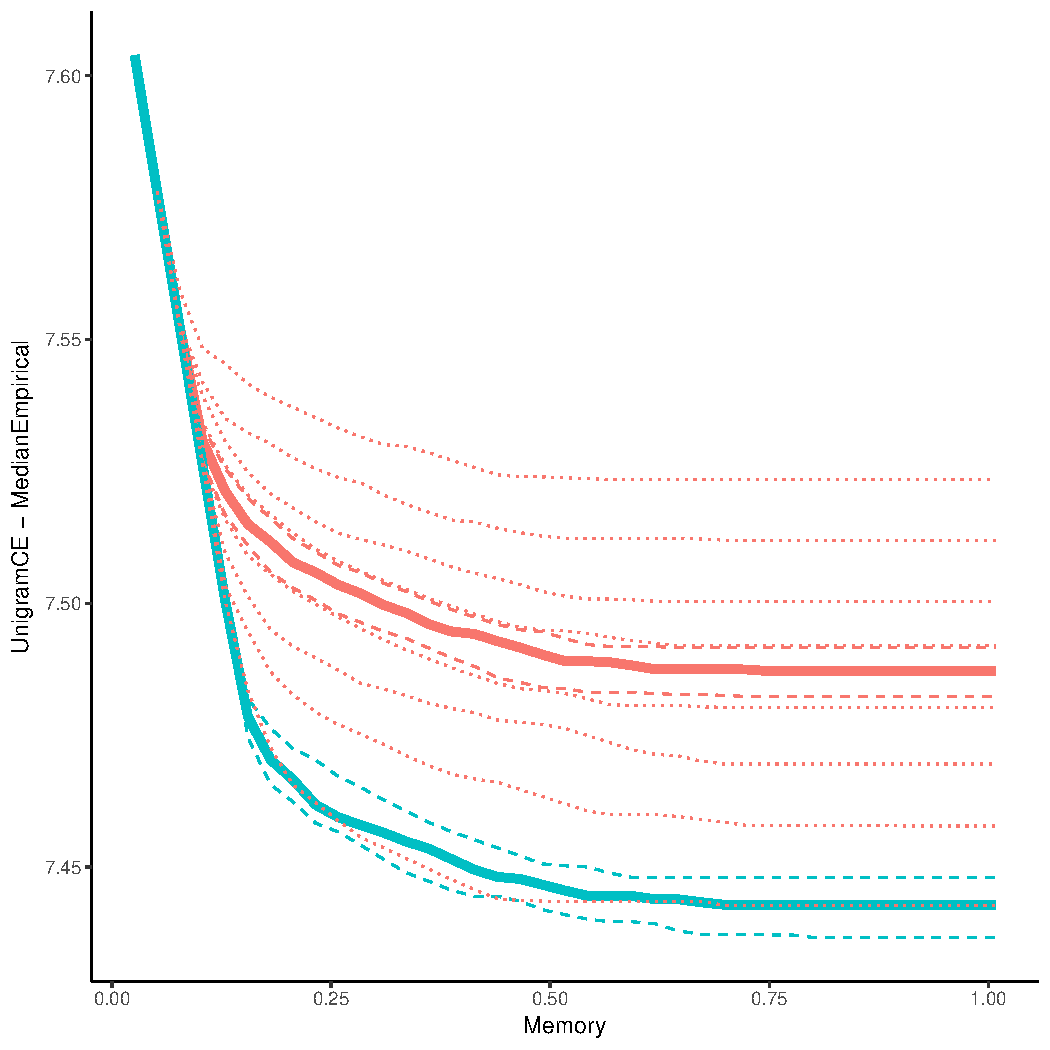
\includegraphics[width=0.25\textwidth]{neural/figures/Armenian-Adap-listener-surprisal-memory-MEDIANS_QUANTILES_onlyWordForms_boundedVocab_REAL.pdf}
 \\ 
Bambara & Basque & Breton & Bulgarian
 \\ 
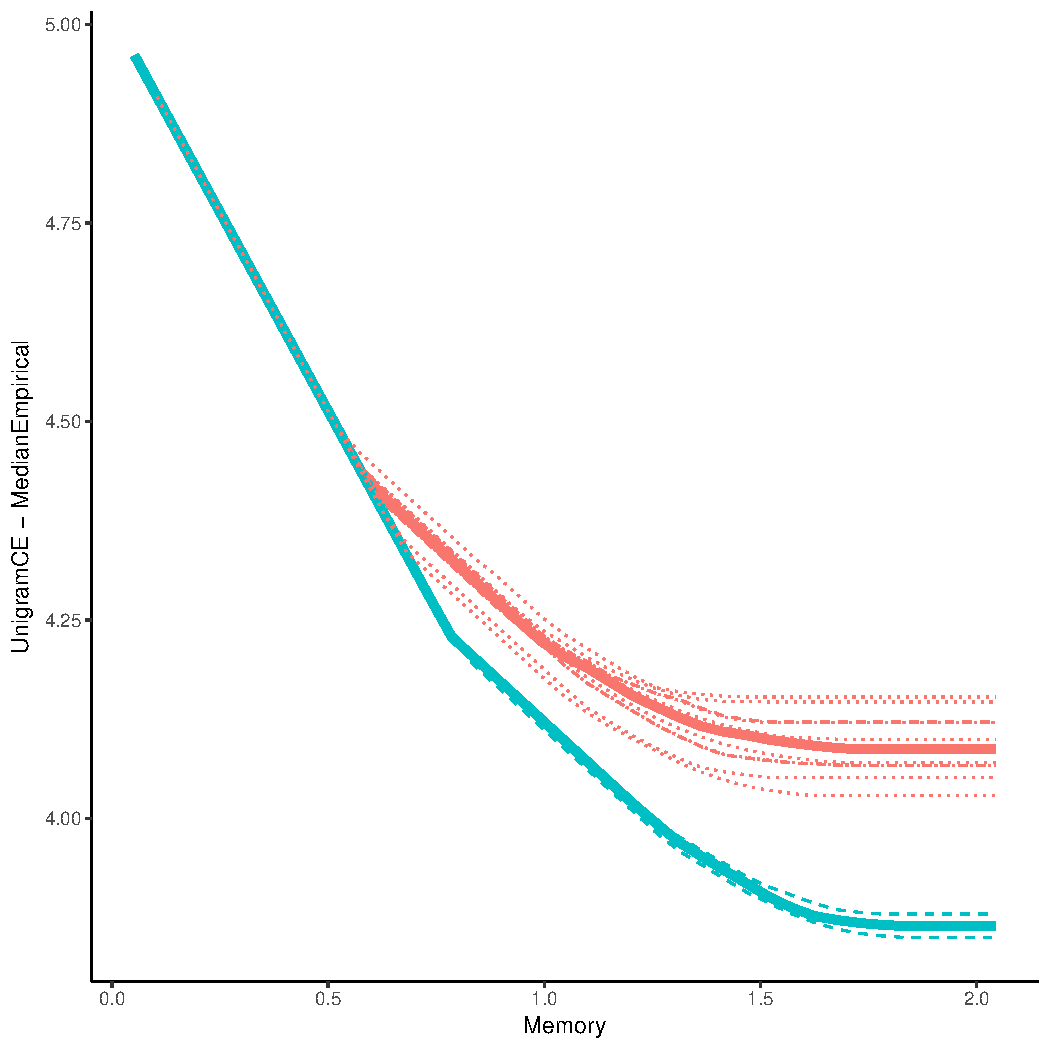
\includegraphics[width=0.25\textwidth]{neural/figures/Bambara-Adap-listener-surprisal-memory-MEDIANS_QUANTILES_onlyWordForms_boundedVocab_REAL.pdf} & 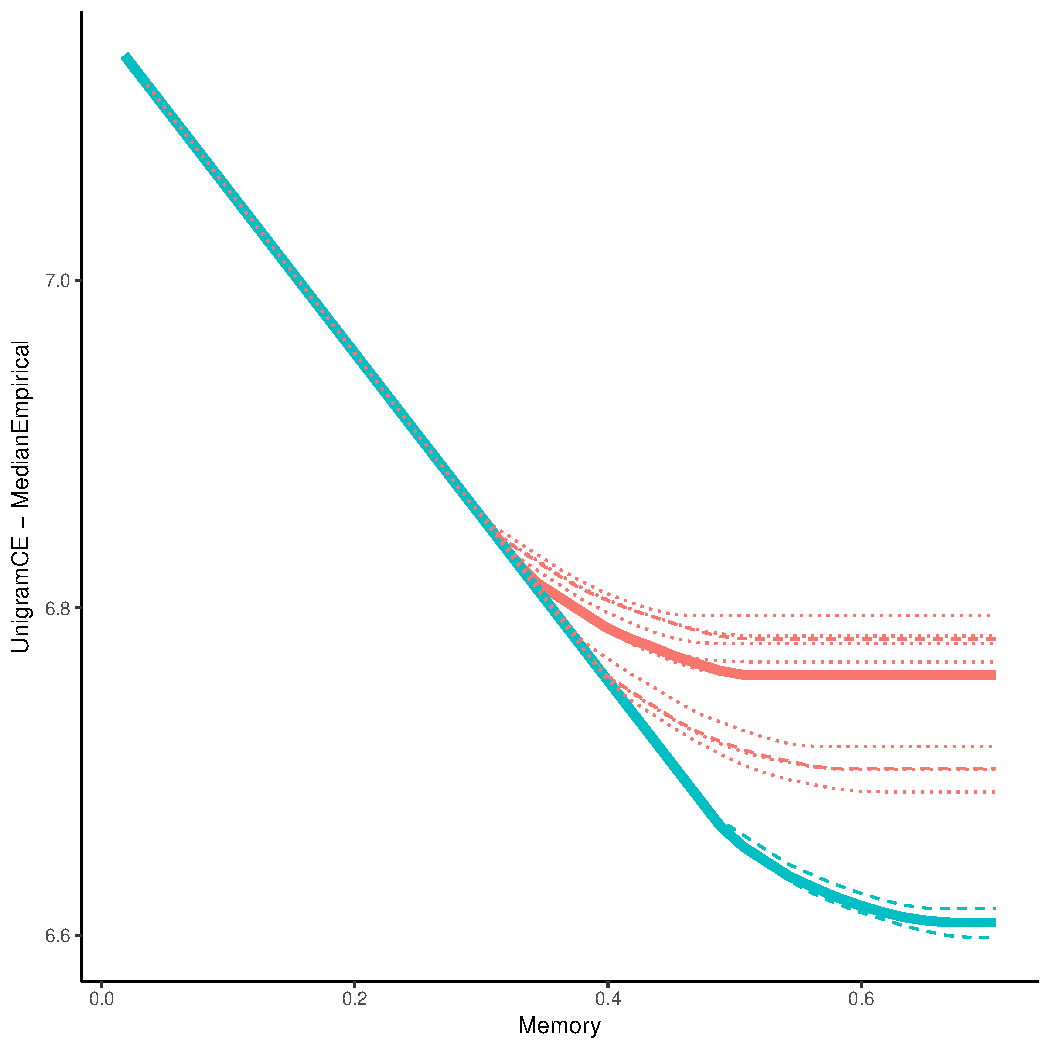
\includegraphics[width=0.25\textwidth]{neural/figures/Basque-listener-surprisal-memory-MEDIANS_QUANTILES_onlyWordForms_boundedVocab_REAL.pdf} & 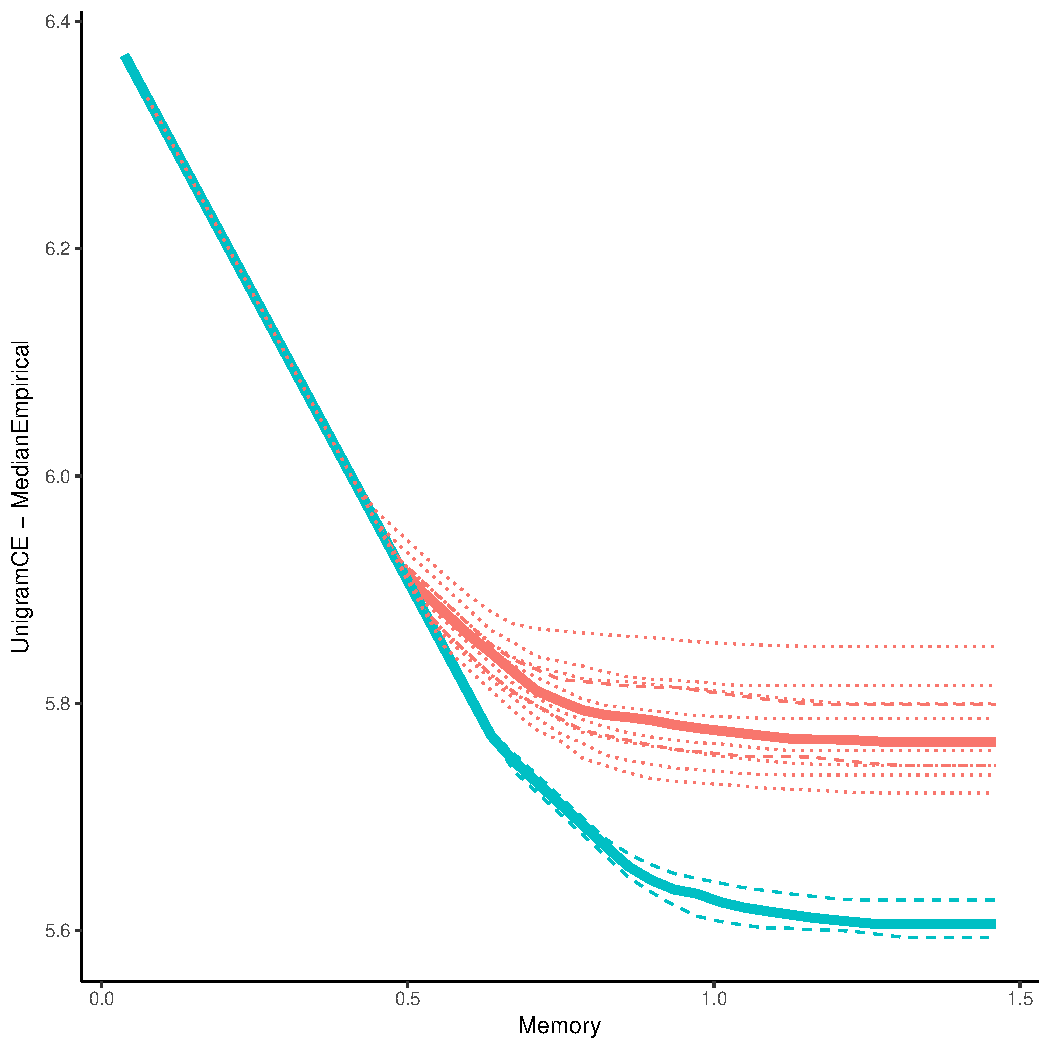
\includegraphics[width=0.25\textwidth]{neural/figures/Breton-Adap-listener-surprisal-memory-MEDIANS_QUANTILES_onlyWordForms_boundedVocab_REAL.pdf} & 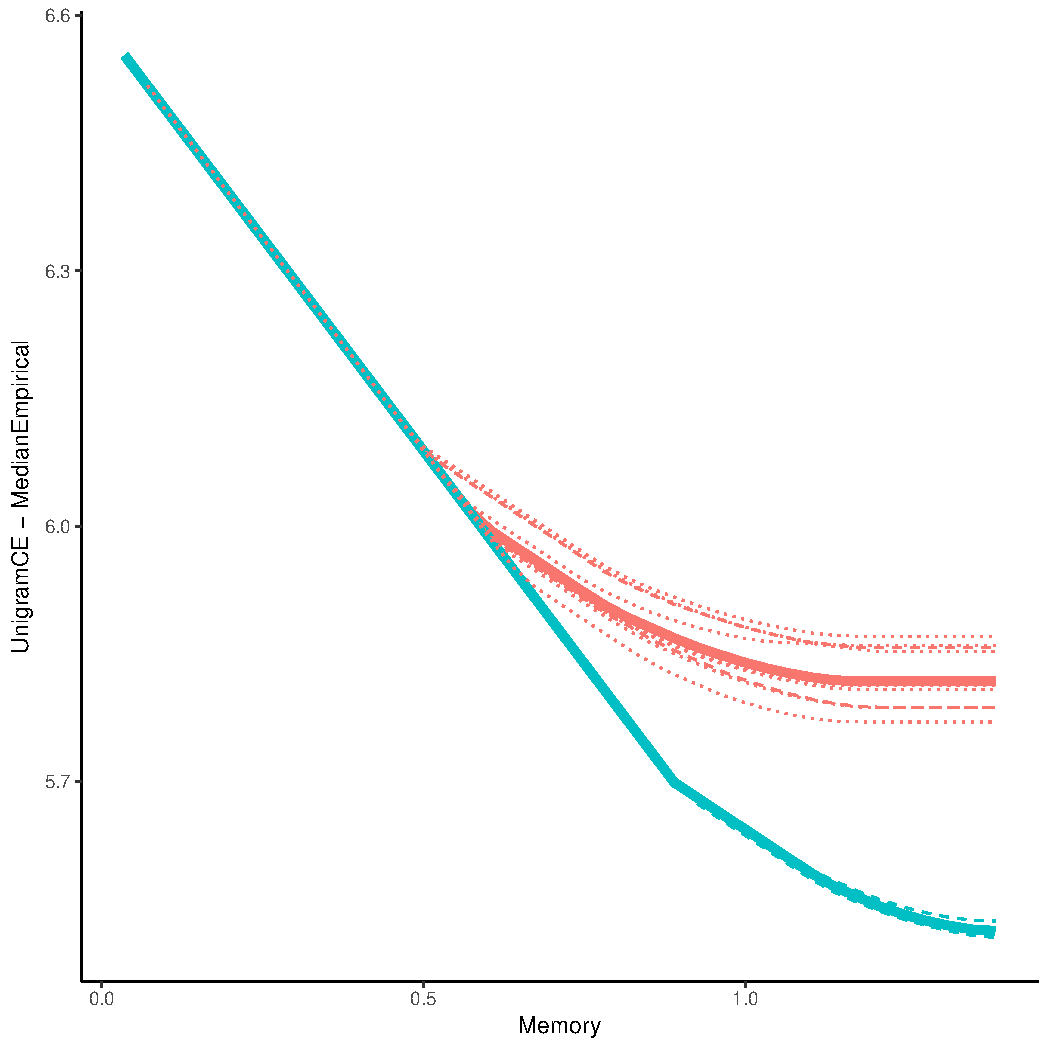
\includegraphics[width=0.25\textwidth]{neural/figures/Bulgarian-listener-surprisal-memory-MEDIANS_QUANTILES_onlyWordForms_boundedVocab_REAL.pdf}
 \\ 
Buryat & Cantonese & Catalan & Chinese
 \\ 
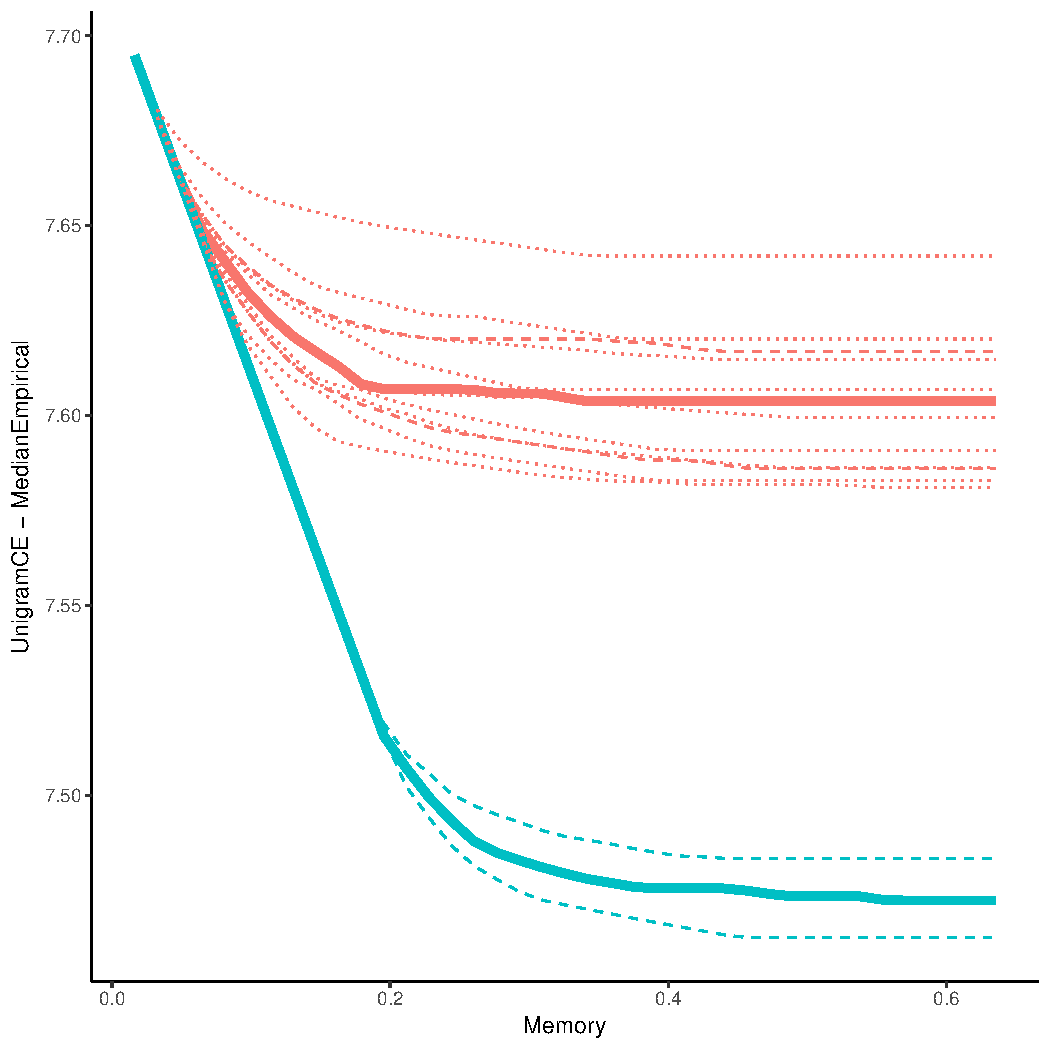
\includegraphics[width=0.25\textwidth]{neural/figures/Buryat-Adap-listener-surprisal-memory-MEDIANS_QUANTILES_onlyWordForms_boundedVocab_REAL.pdf} & 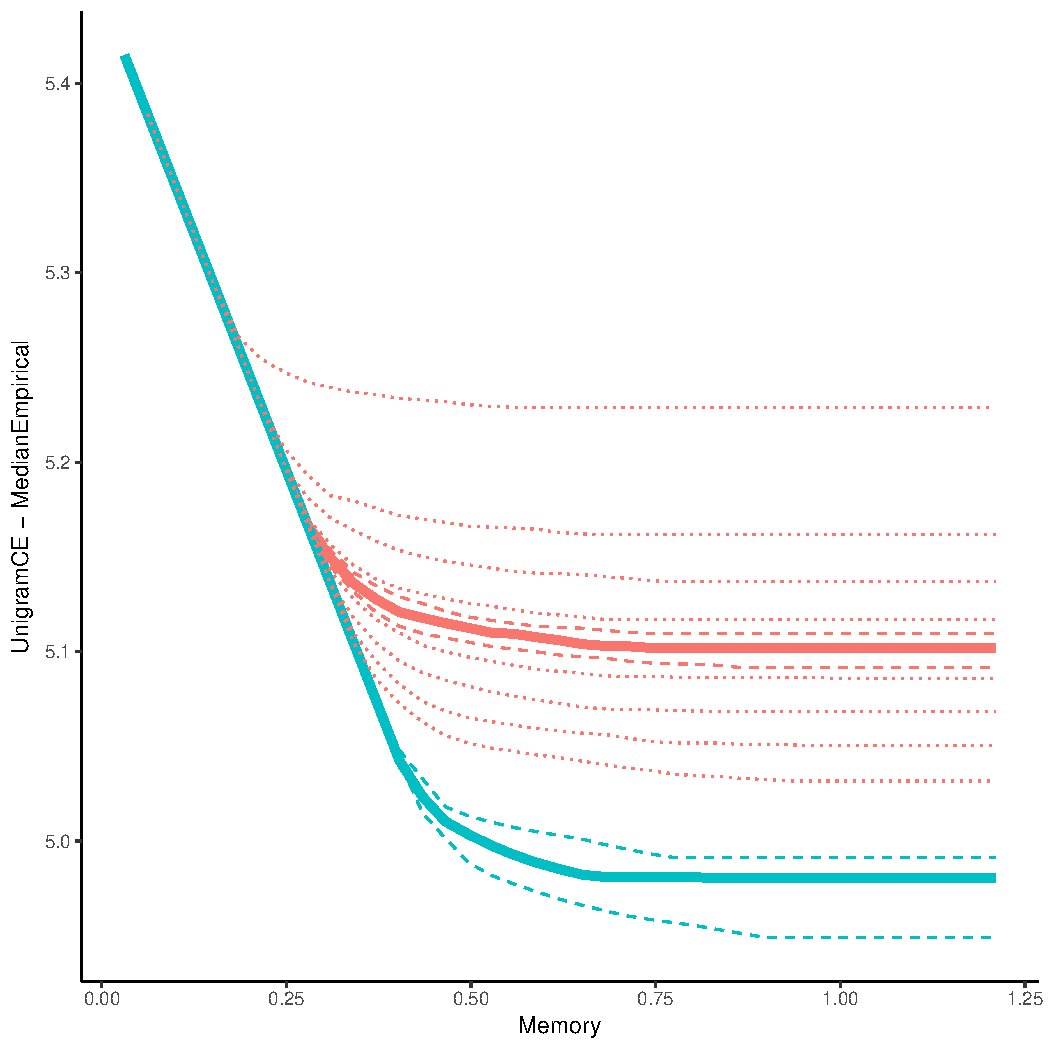
\includegraphics[width=0.25\textwidth]{neural/figures/Cantonese-Adap-listener-surprisal-memory-MEDIANS_QUANTILES_onlyWordForms_boundedVocab_REAL.pdf} & 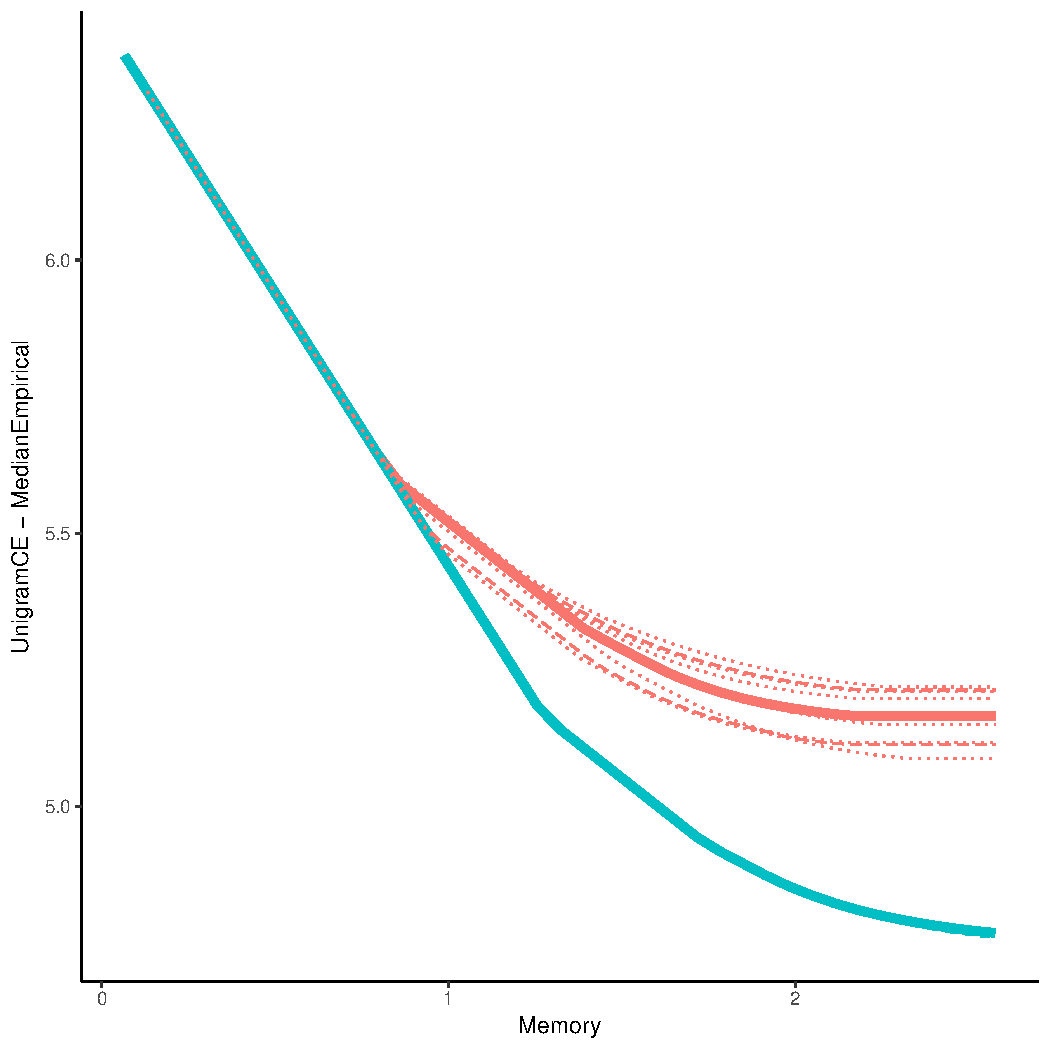
\includegraphics[width=0.25\textwidth]{neural/figures/Catalan-listener-surprisal-memory-MEDIANS_QUANTILES_onlyWordForms_boundedVocab_REAL.pdf} & 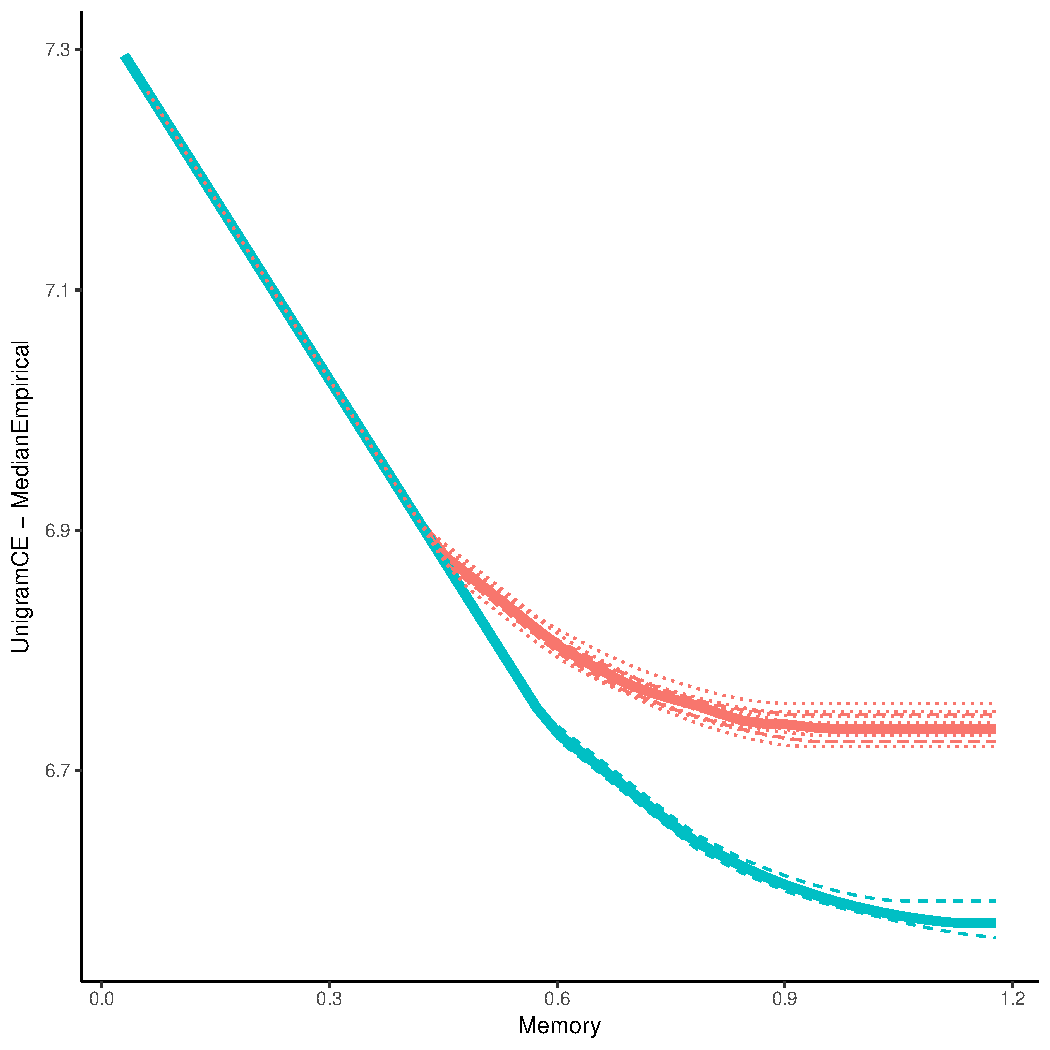
\includegraphics[width=0.25\textwidth]{neural/figures/Chinese-listener-surprisal-memory-MEDIANS_QUANTILES_onlyWordForms_boundedVocab_REAL.pdf}
 \\ 
Croatian & Czech & Danish & Dutch
 \\ 
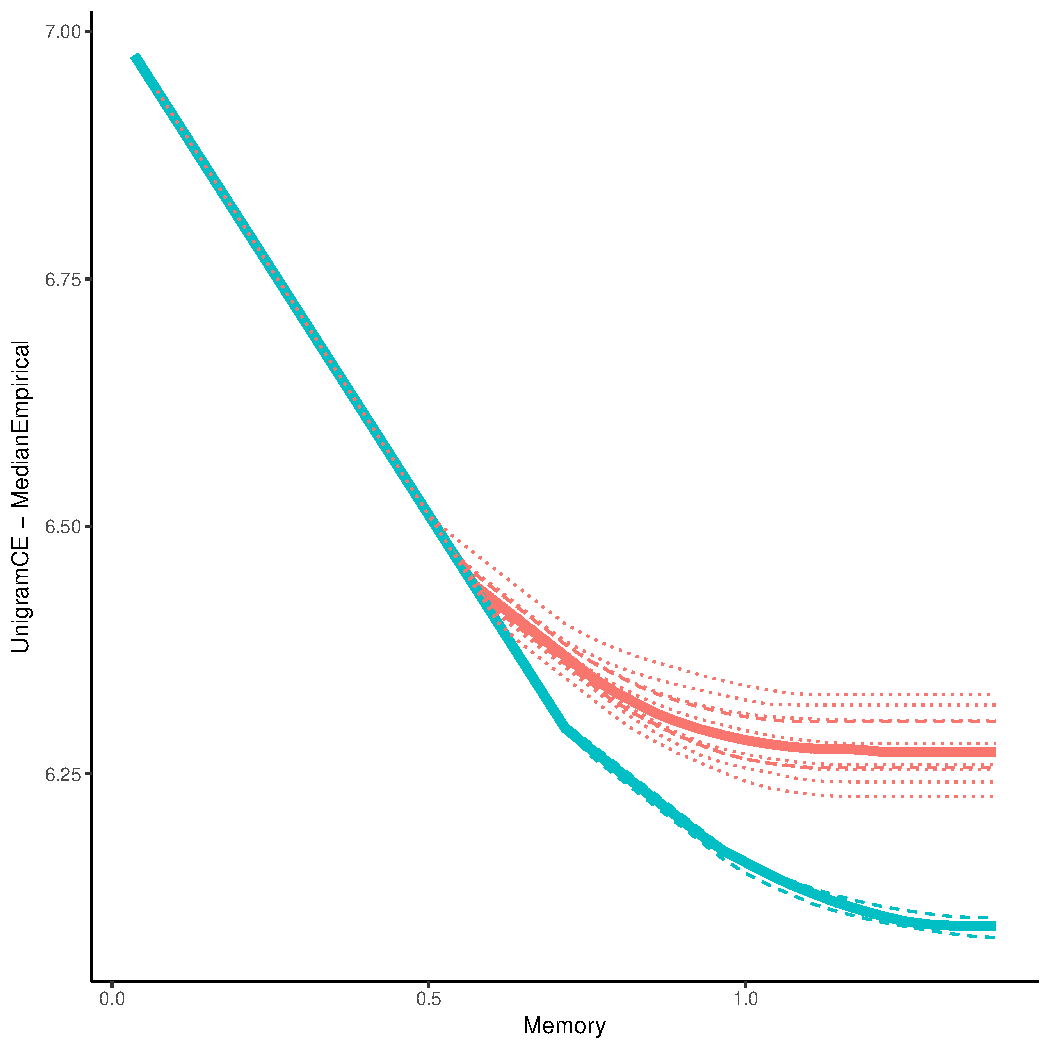
\includegraphics[width=0.25\textwidth]{neural/figures/Croatian-listener-surprisal-memory-MEDIANS_QUANTILES_onlyWordForms_boundedVocab_REAL.pdf} & 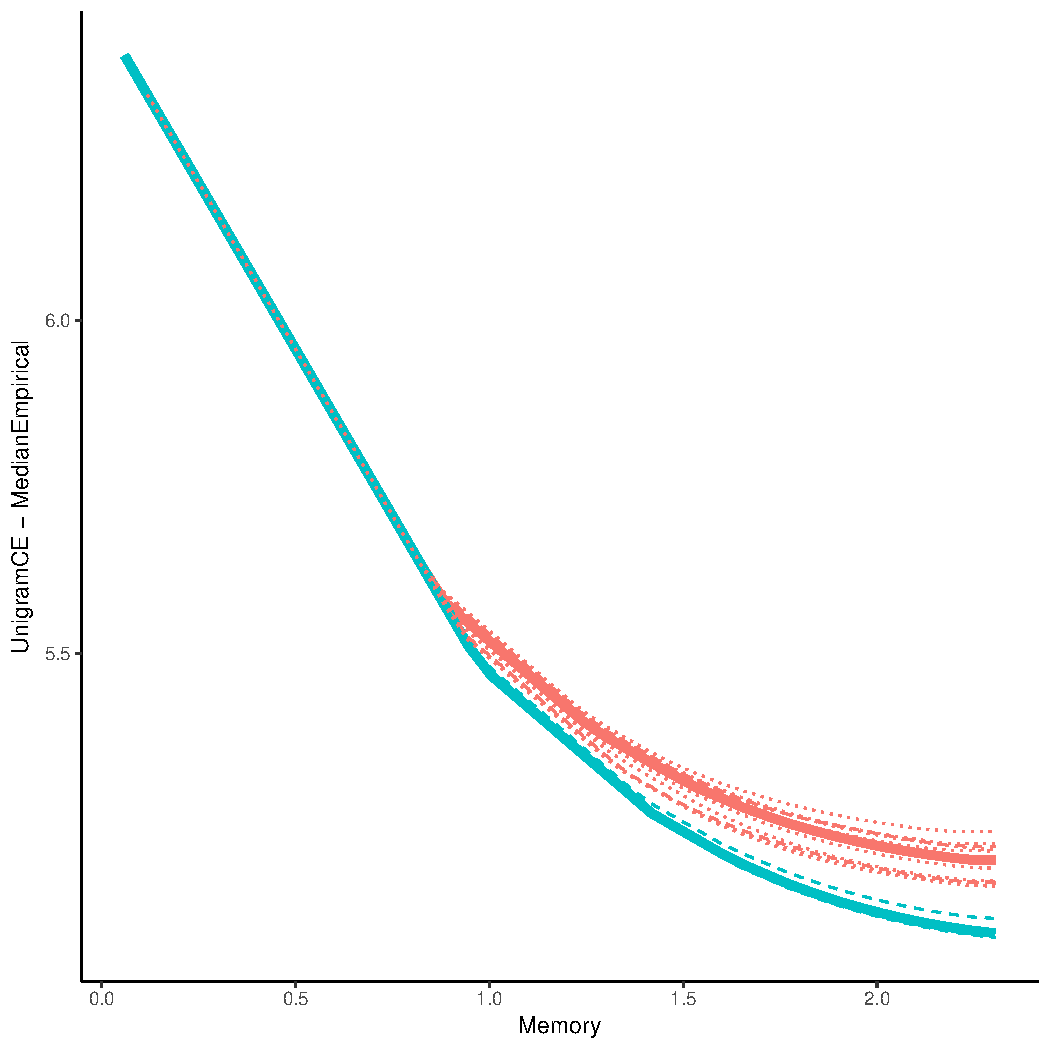
\includegraphics[width=0.25\textwidth]{neural/figures/Czech-listener-surprisal-memory-MEDIANS_QUANTILES_onlyWordForms_boundedVocab_REAL.pdf} & 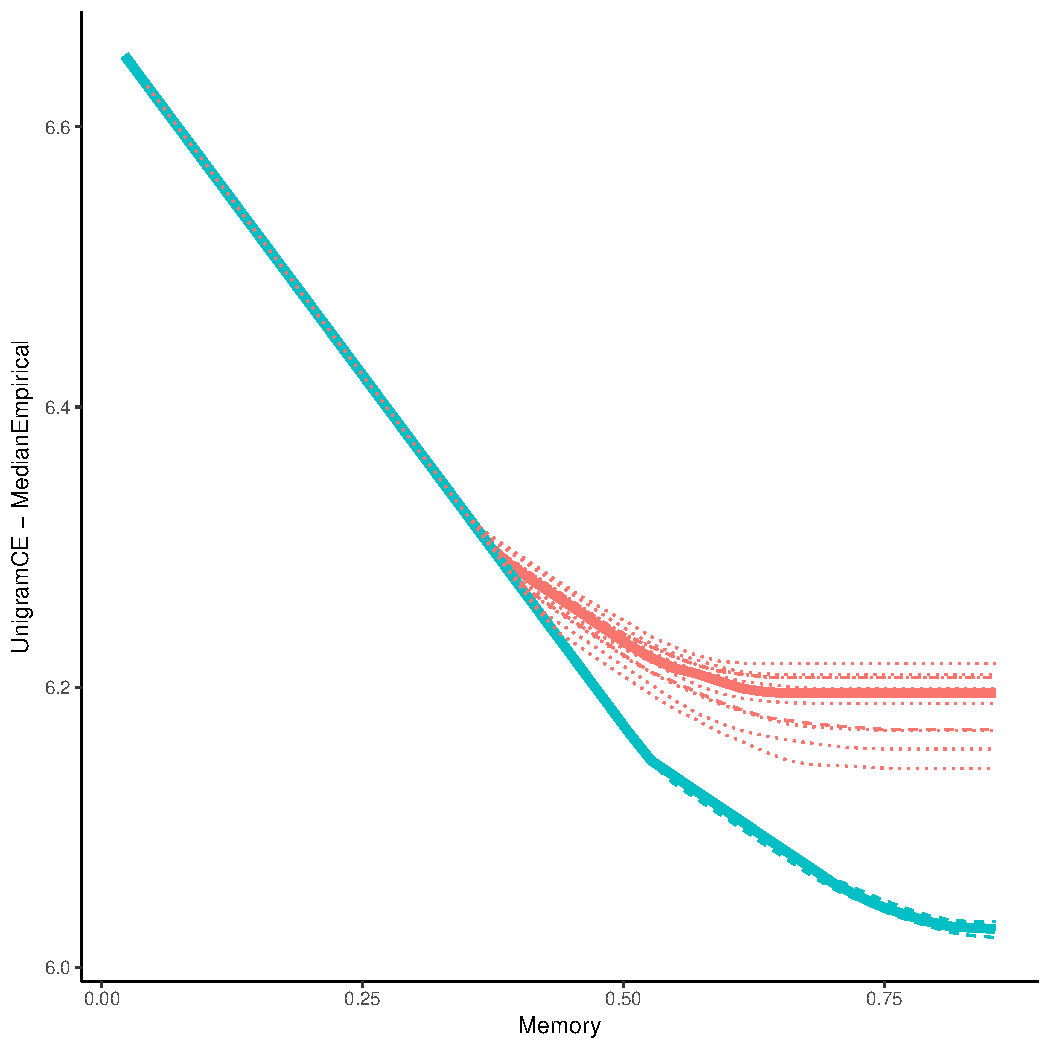
\includegraphics[width=0.25\textwidth]{neural/figures/Danish-listener-surprisal-memory-MEDIANS_QUANTILES_onlyWordForms_boundedVocab_REAL.pdf} & 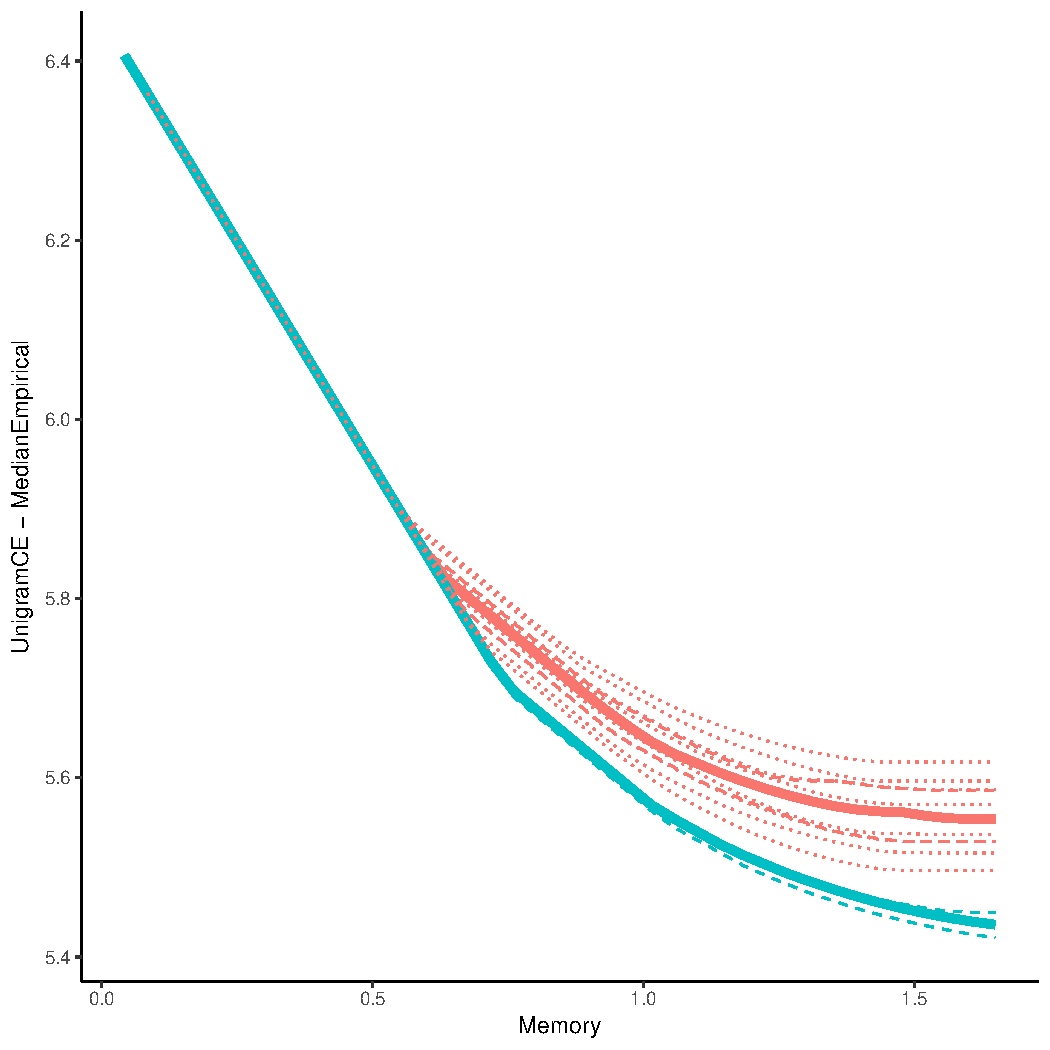
\includegraphics[width=0.25\textwidth]{neural/figures/Dutch-listener-surprisal-memory-MEDIANS_QUANTILES_onlyWordForms_boundedVocab_REAL.pdf}
 \\ 

\end{longtable}
	\captionof{figure}{Medians: For each memory budget, we provide the median surprisal for real and random languages. Solid lines indicate sample medians, dashed lines indicate 95 $\%$ confidence intervals for the population median, dotted lines indicate empirical quantiles ($10\%, 20\%, \dots, 80\%, 90\%$). Green: Random baselines; blue: real language; red: maximum-likelihood grammars fit to real orderings.}\label{tab:medians}
\end{center}

\begin{center}
\begin{longtable}{ccccccccccccccclll}
English & Erzya & Estonian & Faroese
 \\ 
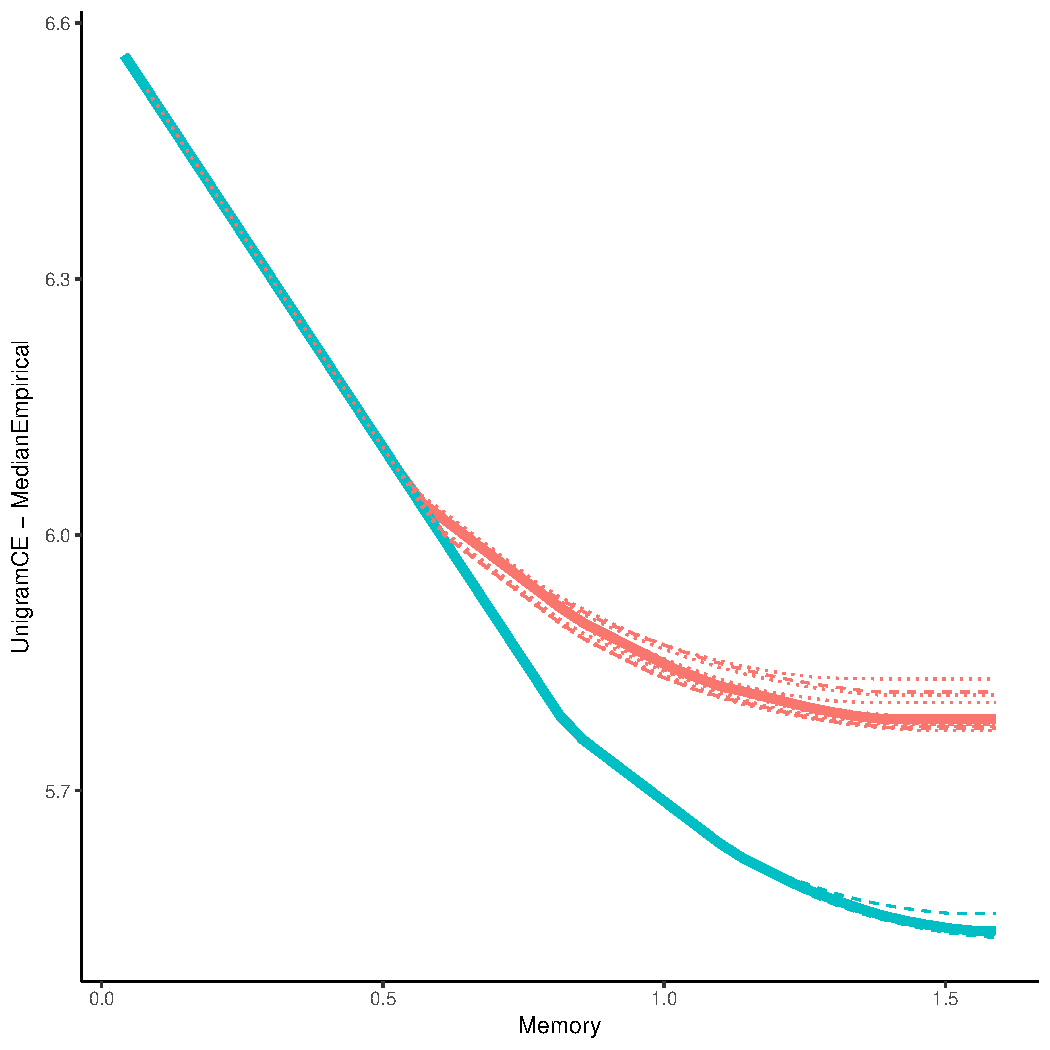
\includegraphics[width=0.25\textwidth]{neural/figures/English-listener-surprisal-memory-MEDIANS_QUANTILES_onlyWordForms_boundedVocab_REAL.pdf} & 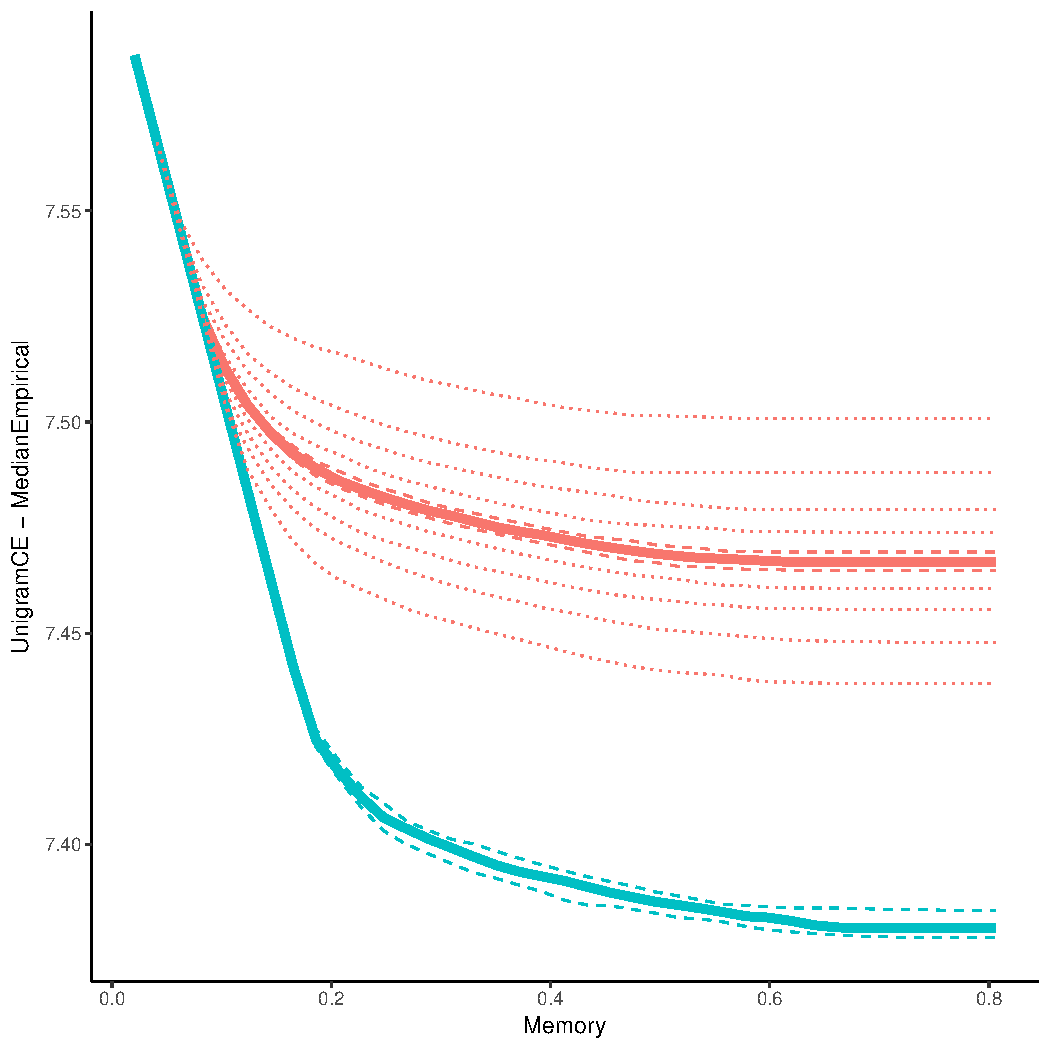
\includegraphics[width=0.25\textwidth]{neural/figures/Erzya-Adap-listener-surprisal-memory-MEDIANS_QUANTILES_onlyWordForms_boundedVocab_REAL.pdf} & 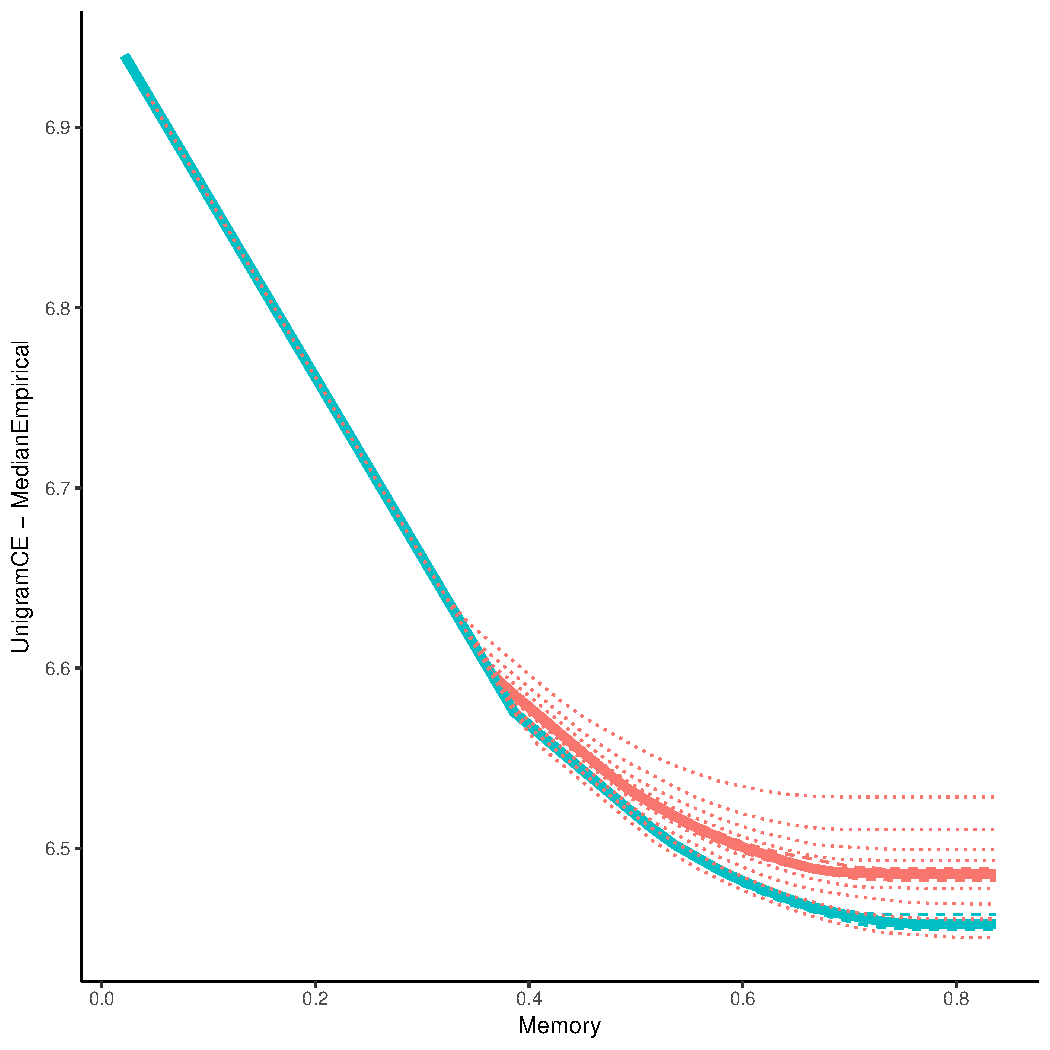
\includegraphics[width=0.25\textwidth]{neural/figures/Estonian-listener-surprisal-memory-MEDIANS_QUANTILES_onlyWordForms_boundedVocab_REAL.pdf} & 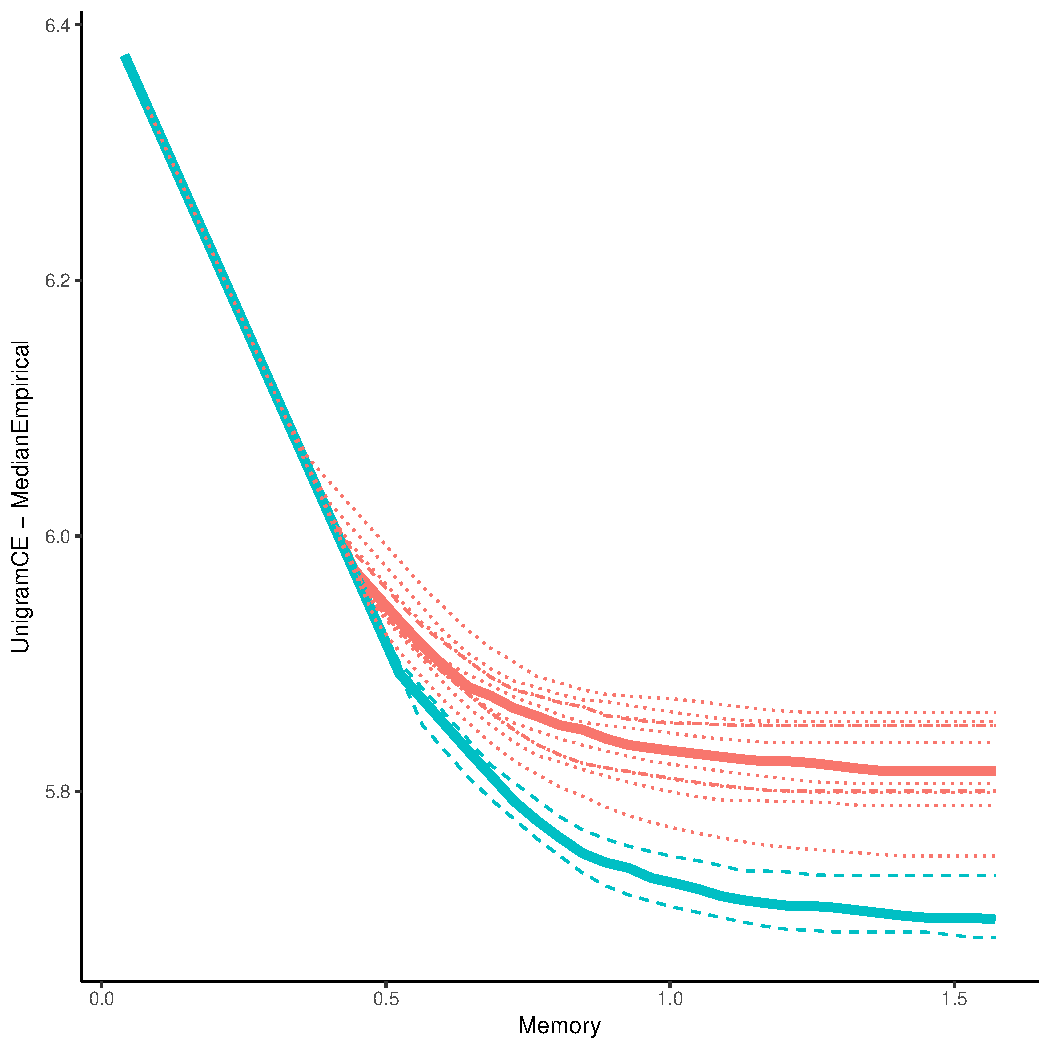
\includegraphics[width=0.25\textwidth]{neural/figures/Faroese-Adap-listener-surprisal-memory-MEDIANS_QUANTILES_onlyWordForms_boundedVocab_REAL.pdf}
 \\ 
Finnish & French & German & Greek
 \\ 
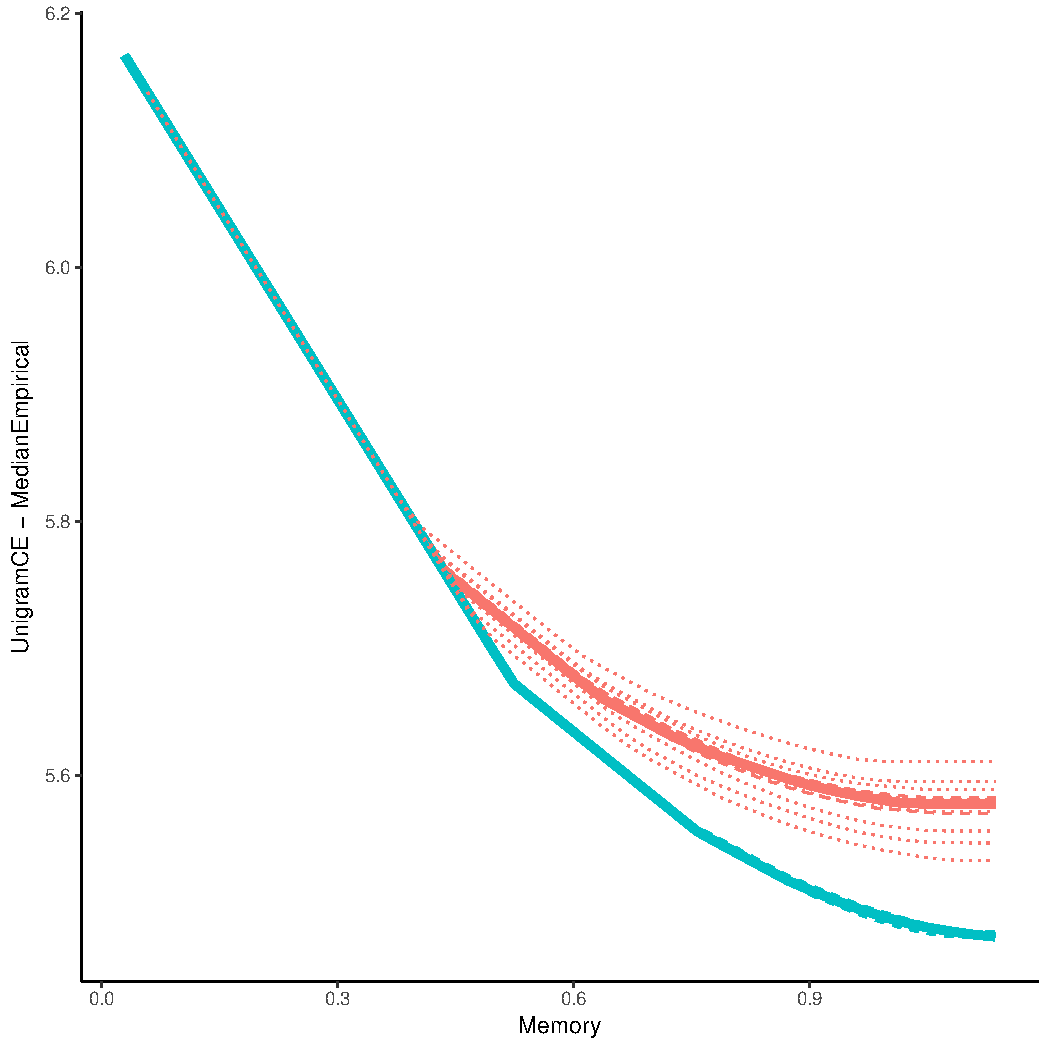
\includegraphics[width=0.25\textwidth]{neural/figures/Finnish-listener-surprisal-memory-MEDIANS_QUANTILES_onlyWordForms_boundedVocab_REAL.pdf} & 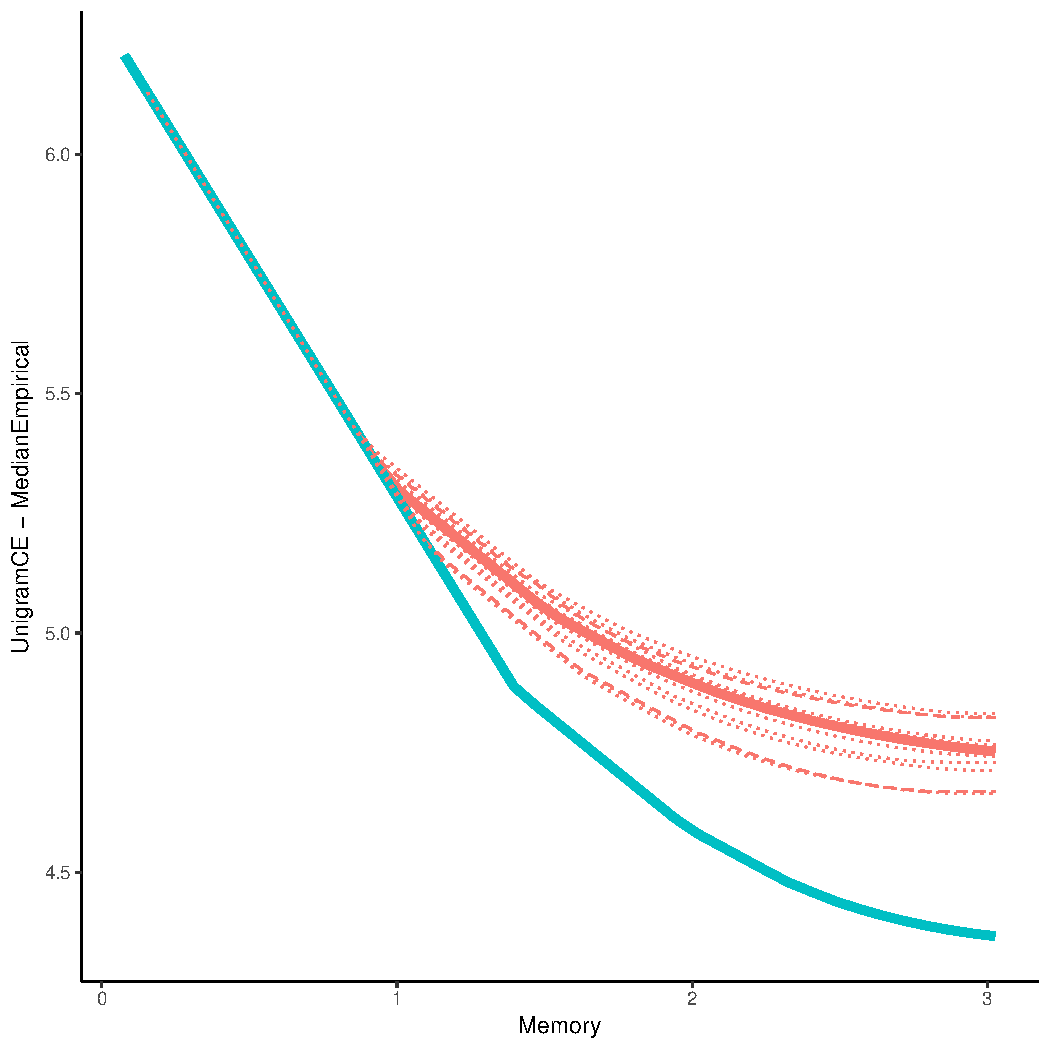
\includegraphics[width=0.25\textwidth]{neural/figures/French-listener-surprisal-memory-MEDIANS_QUANTILES_onlyWordForms_boundedVocab_REAL.pdf} & 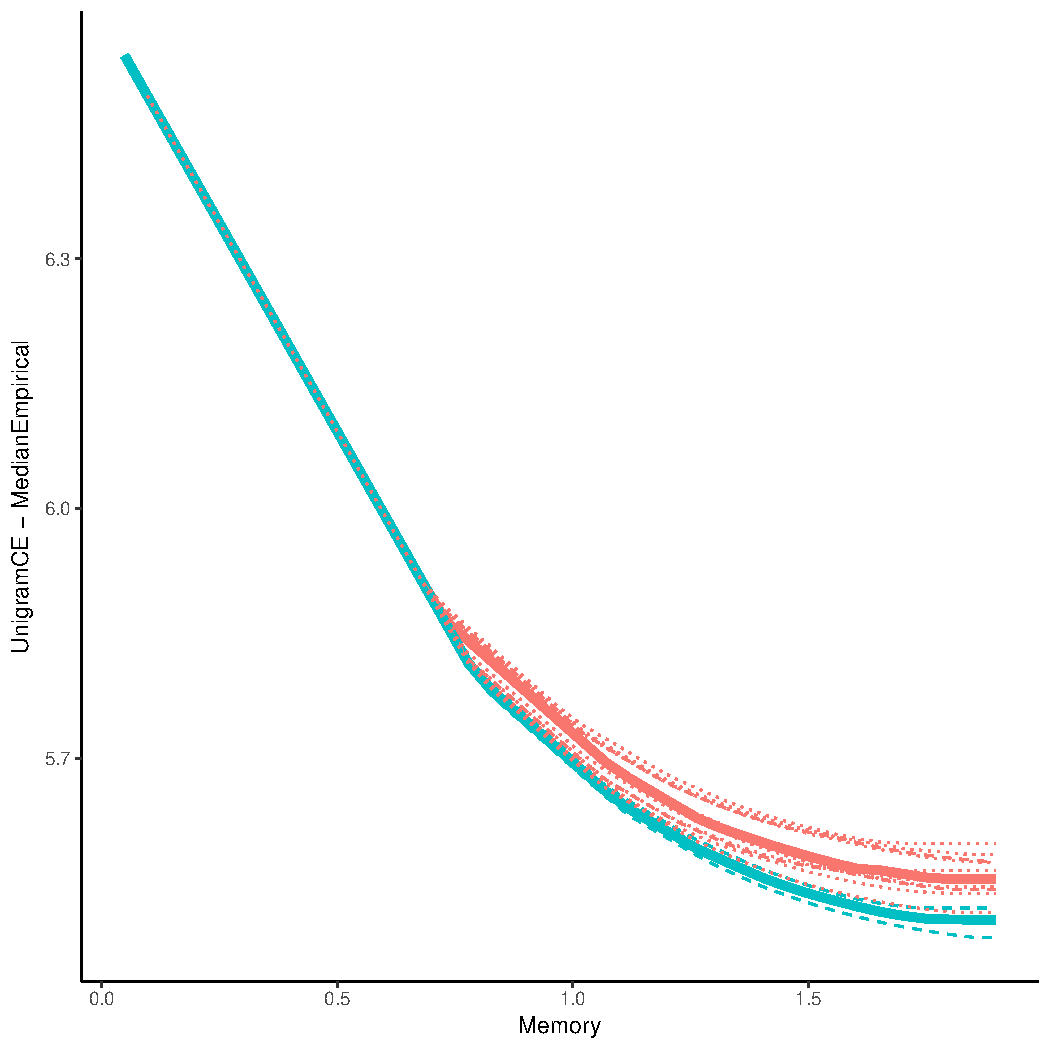
\includegraphics[width=0.25\textwidth]{neural/figures/German-listener-surprisal-memory-MEDIANS_QUANTILES_onlyWordForms_boundedVocab_REAL.pdf} & 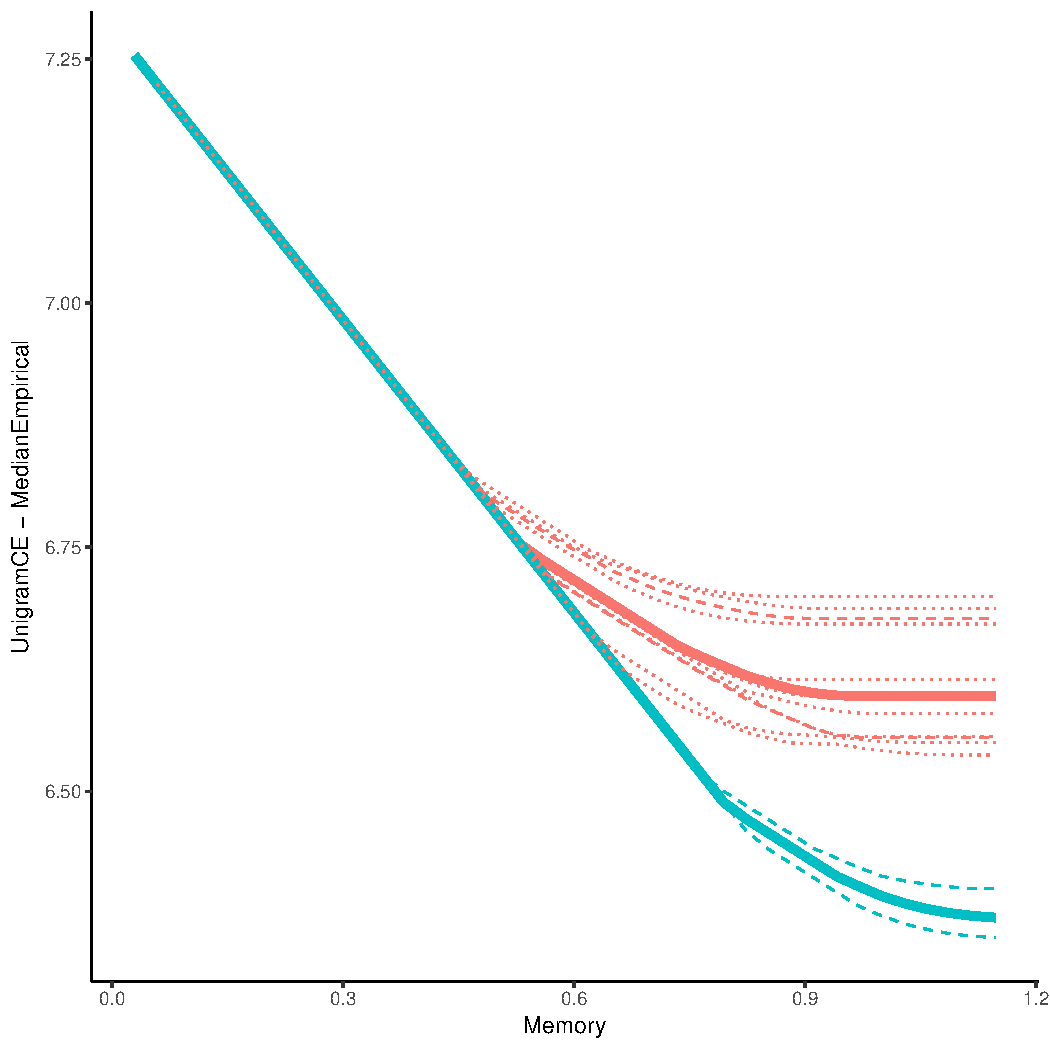
\includegraphics[width=0.25\textwidth]{neural/figures/Greek-listener-surprisal-memory-MEDIANS_QUANTILES_onlyWordForms_boundedVocab_REAL.pdf}
 \\ 
Hebrew & Hindi & Hungarian & Indonesian
 \\ 
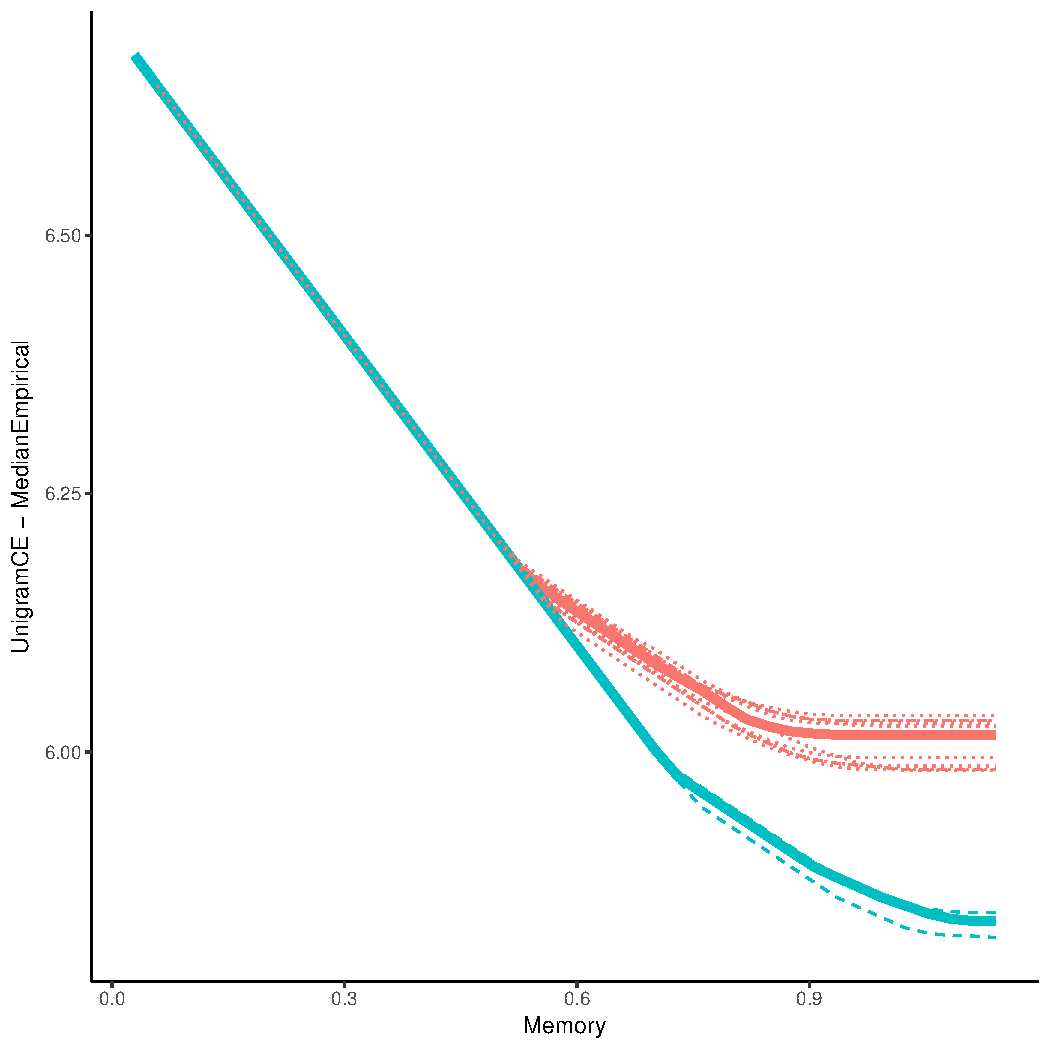
\includegraphics[width=0.25\textwidth]{neural/figures/Hebrew-listener-surprisal-memory-MEDIANS_QUANTILES_onlyWordForms_boundedVocab_REAL.pdf} & 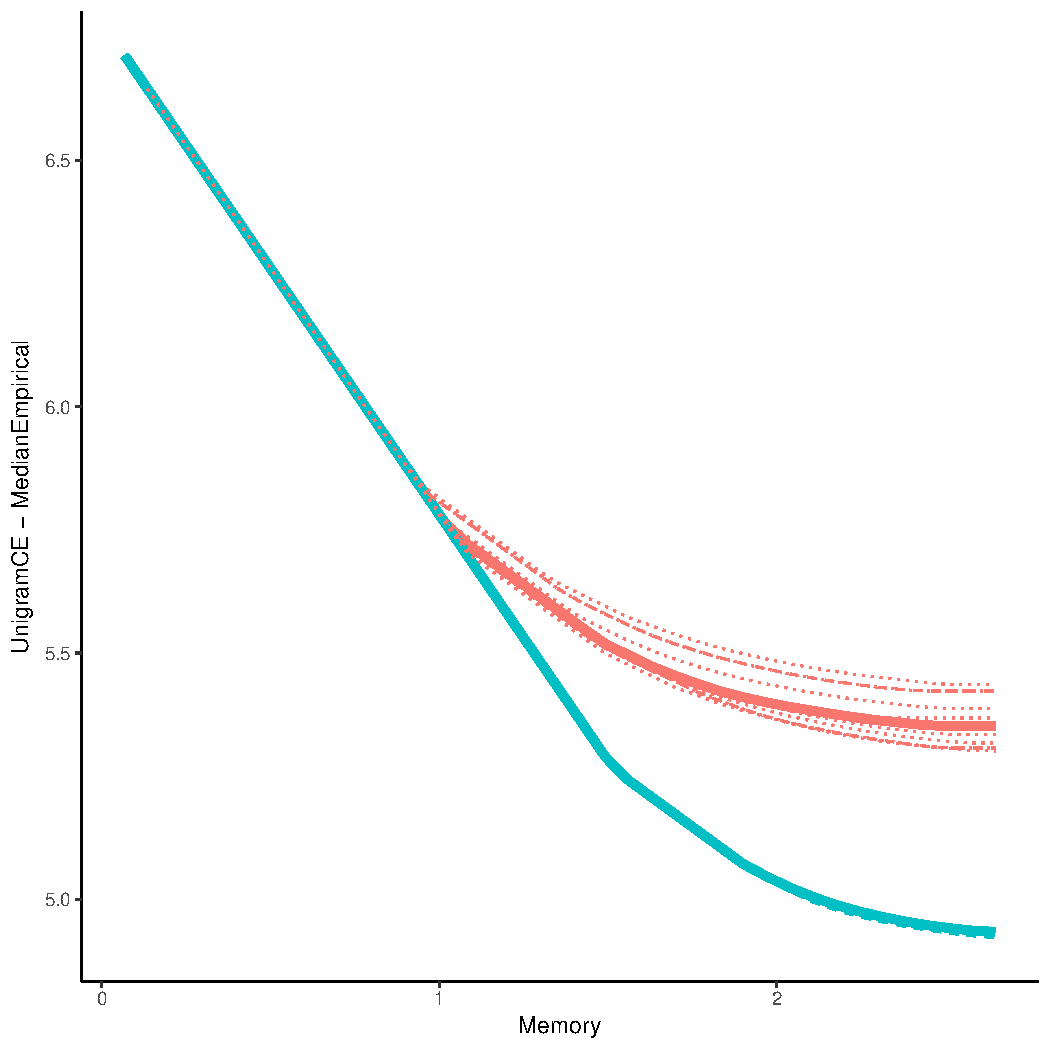
\includegraphics[width=0.25\textwidth]{neural/figures/Hindi-listener-surprisal-memory-MEDIANS_QUANTILES_onlyWordForms_boundedVocab_REAL.pdf} & 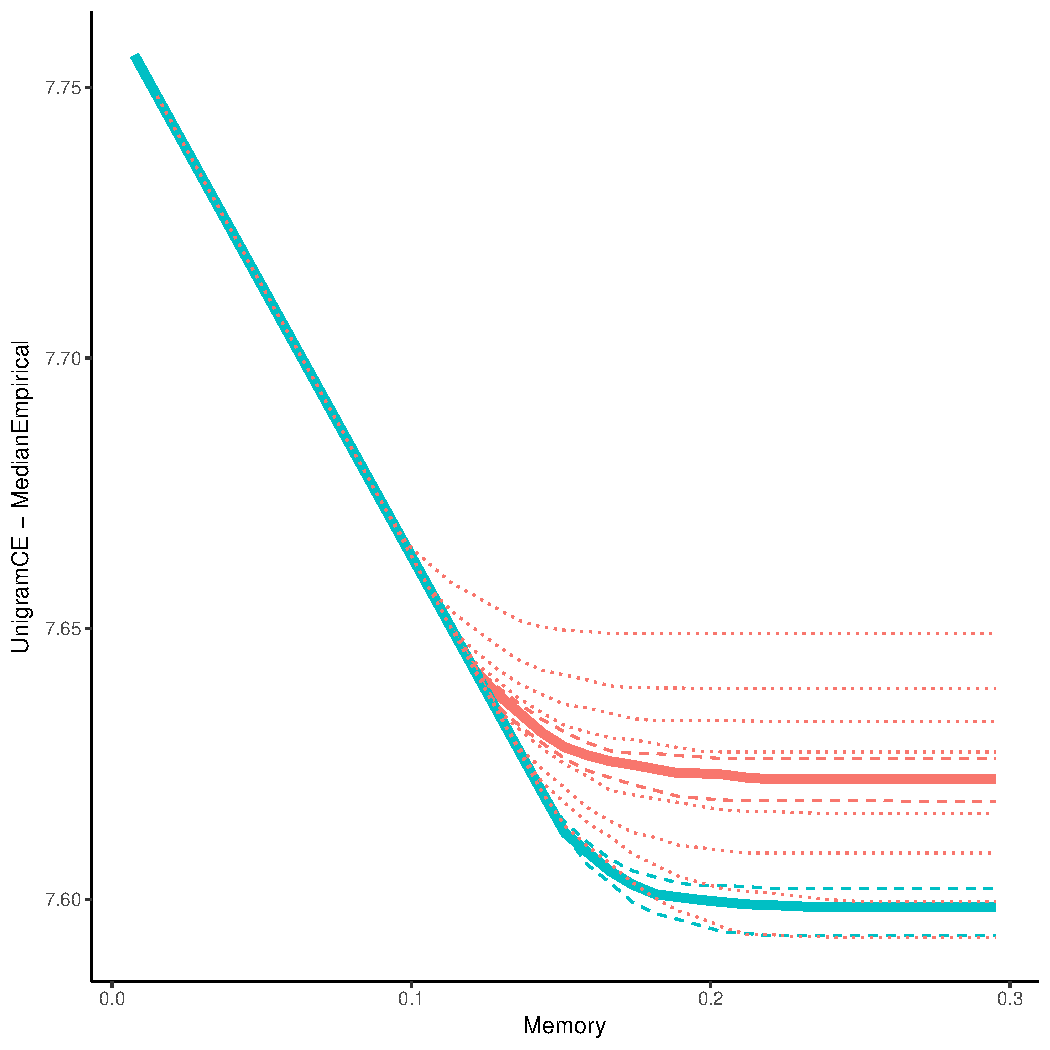
\includegraphics[width=0.25\textwidth]{neural/figures/Hungarian-listener-surprisal-memory-MEDIANS_QUANTILES_onlyWordForms_boundedVocab_REAL.pdf} & 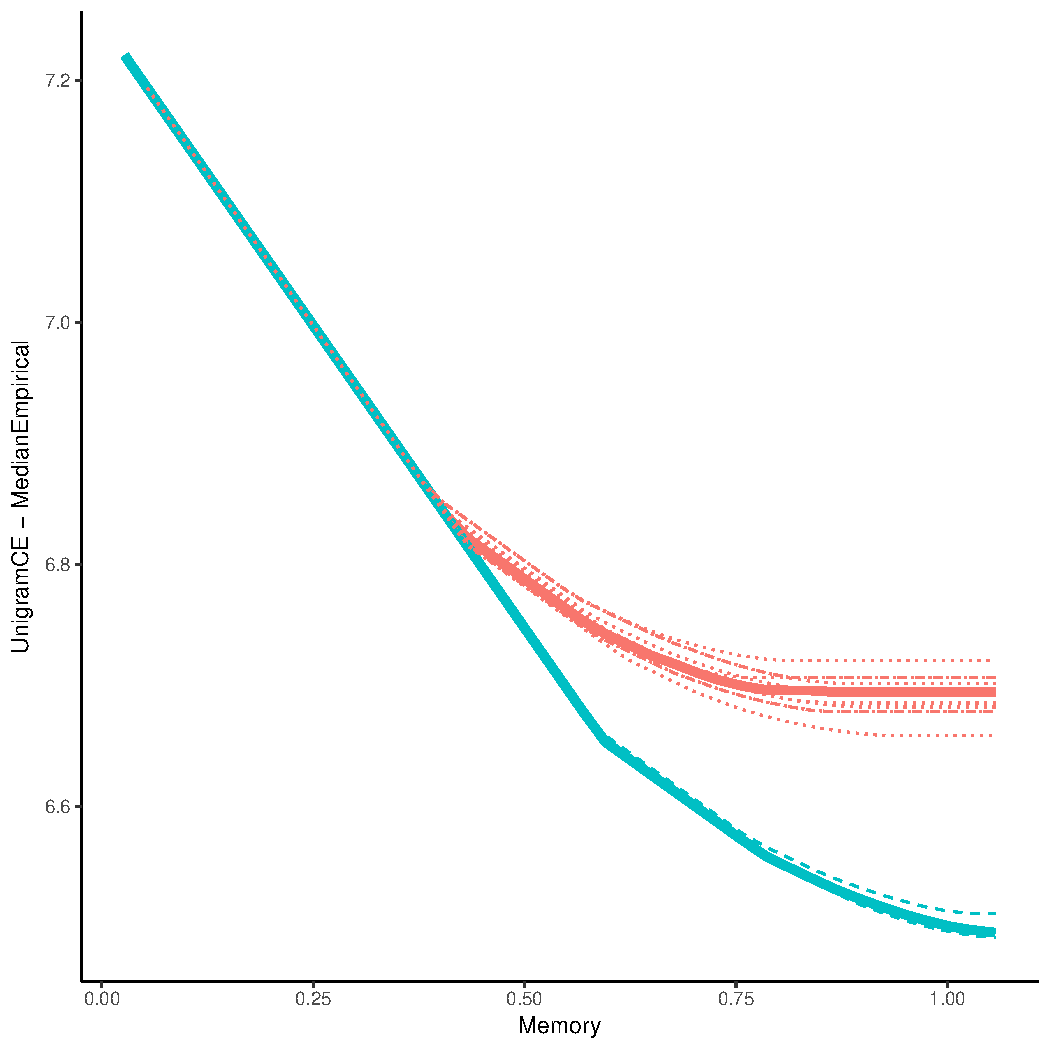
\includegraphics[width=0.25\textwidth]{neural/figures/Indonesian-listener-surprisal-memory-MEDIANS_QUANTILES_onlyWordForms_boundedVocab_REAL.pdf}
 \\ 
Italian & Japanese & Kazakh & Korean
 \\ 
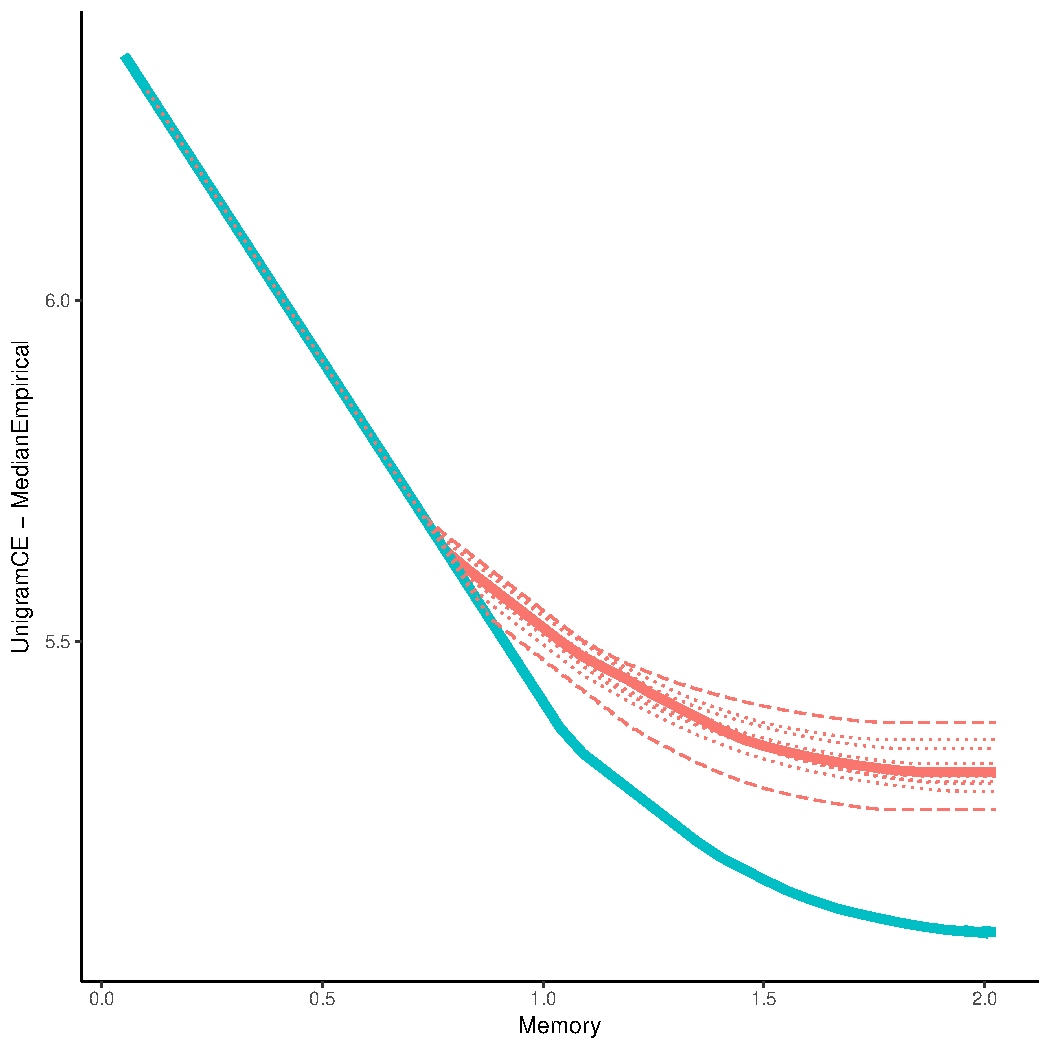
\includegraphics[width=0.25\textwidth]{neural/figures/Italian-listener-surprisal-memory-MEDIANS_QUANTILES_onlyWordForms_boundedVocab_REAL.pdf} & 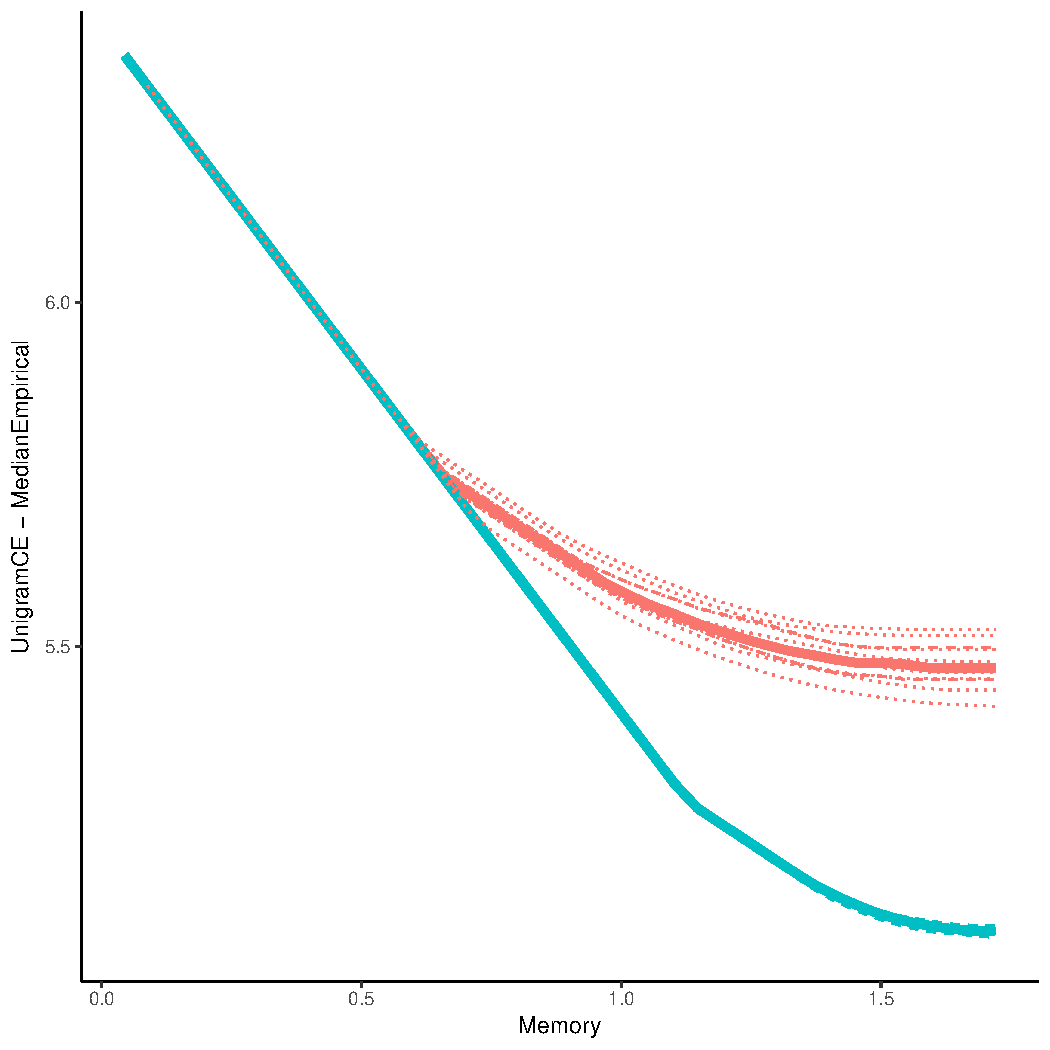
\includegraphics[width=0.25\textwidth]{neural/figures/Japanese-listener-surprisal-memory-MEDIANS_QUANTILES_onlyWordForms_boundedVocab_REAL.pdf} & 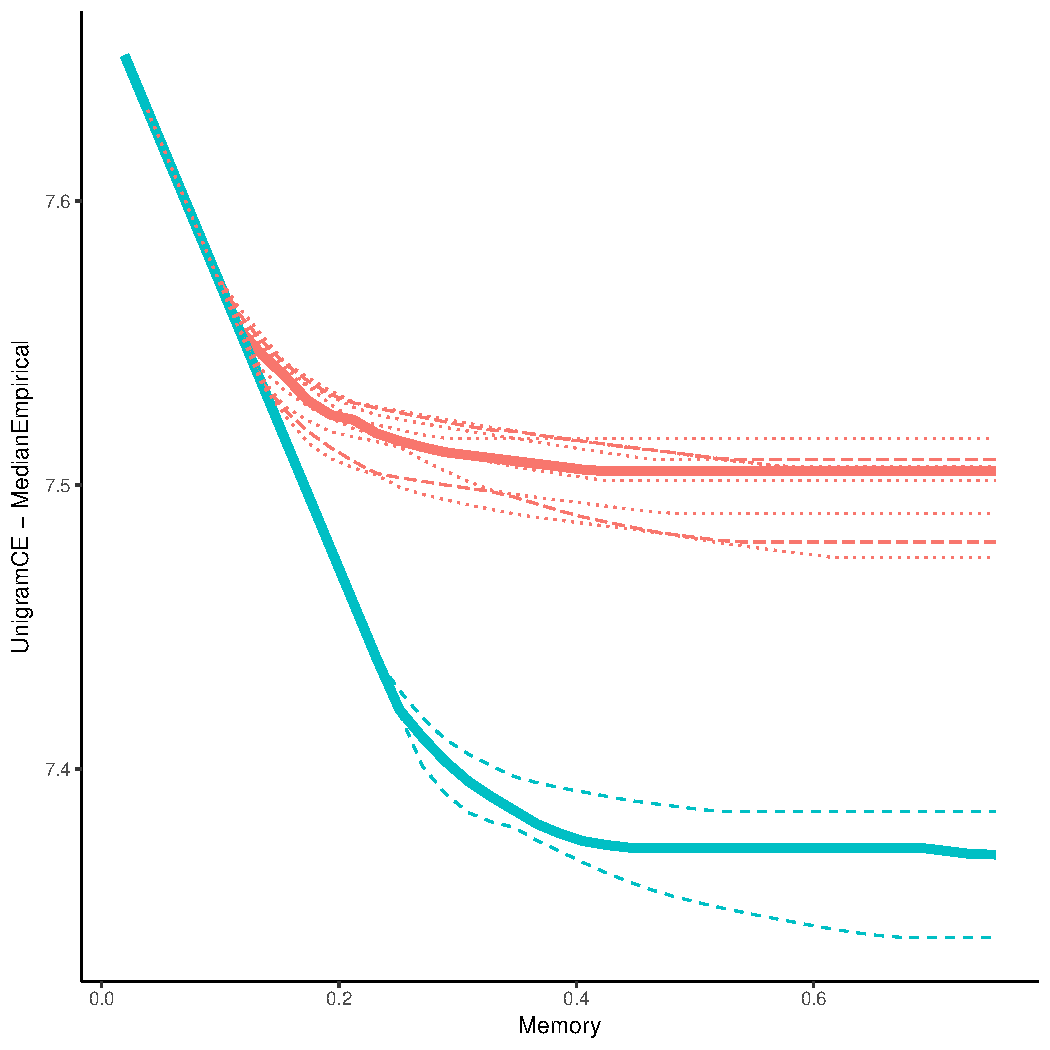
\includegraphics[width=0.25\textwidth]{neural/figures/Kazakh-Adap-listener-surprisal-memory-MEDIANS_QUANTILES_onlyWordForms_boundedVocab_REAL.pdf} & 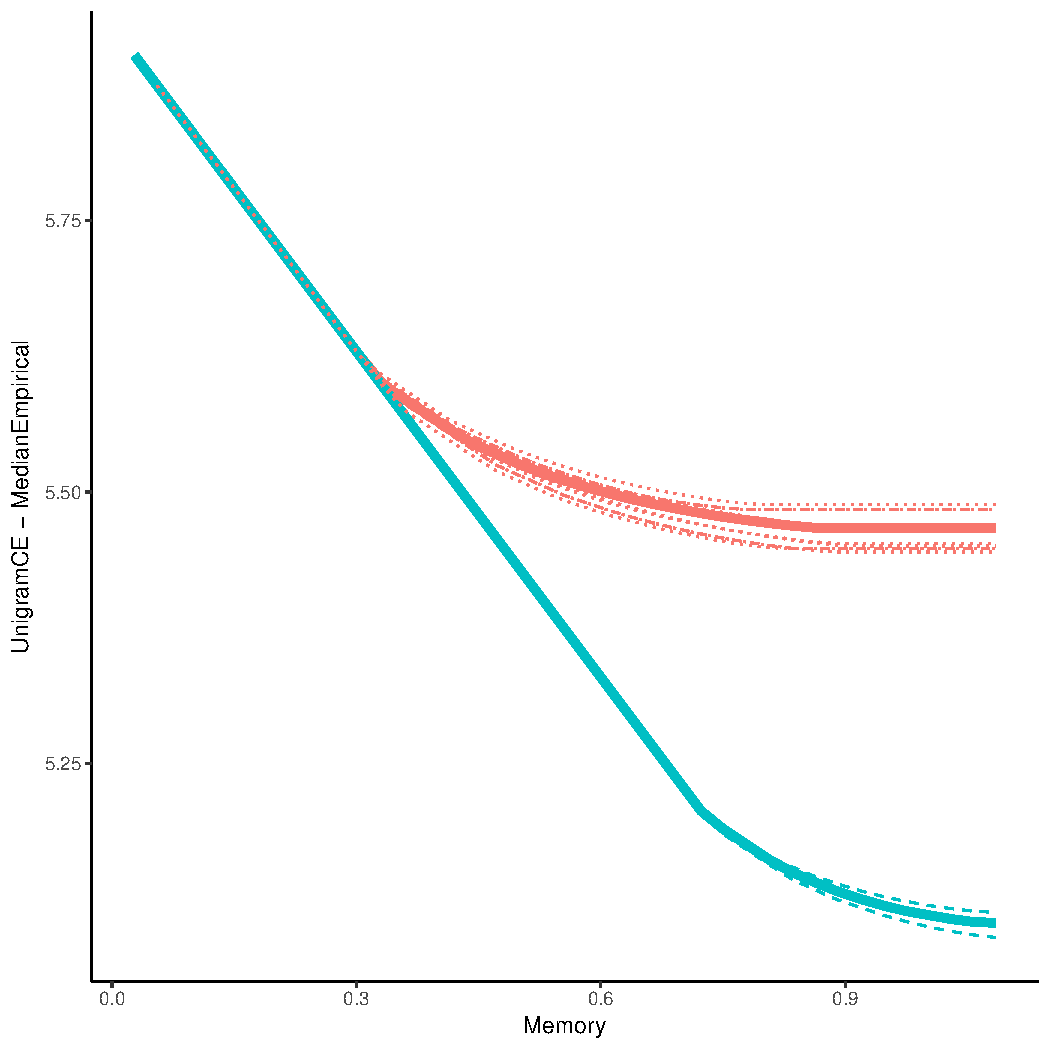
\includegraphics[width=0.25\textwidth]{neural/figures/Korean-listener-surprisal-memory-MEDIANS_QUANTILES_onlyWordForms_boundedVocab_REAL.pdf}
 \\ 

\end{longtable}
	\captionof{figure}{Medians (cont.)}
\end{center}

\begin{center}
\begin{longtable}{ccccccccccccccclll}
Kurmanji & Latvian & Maltese & Naija
 \\ 
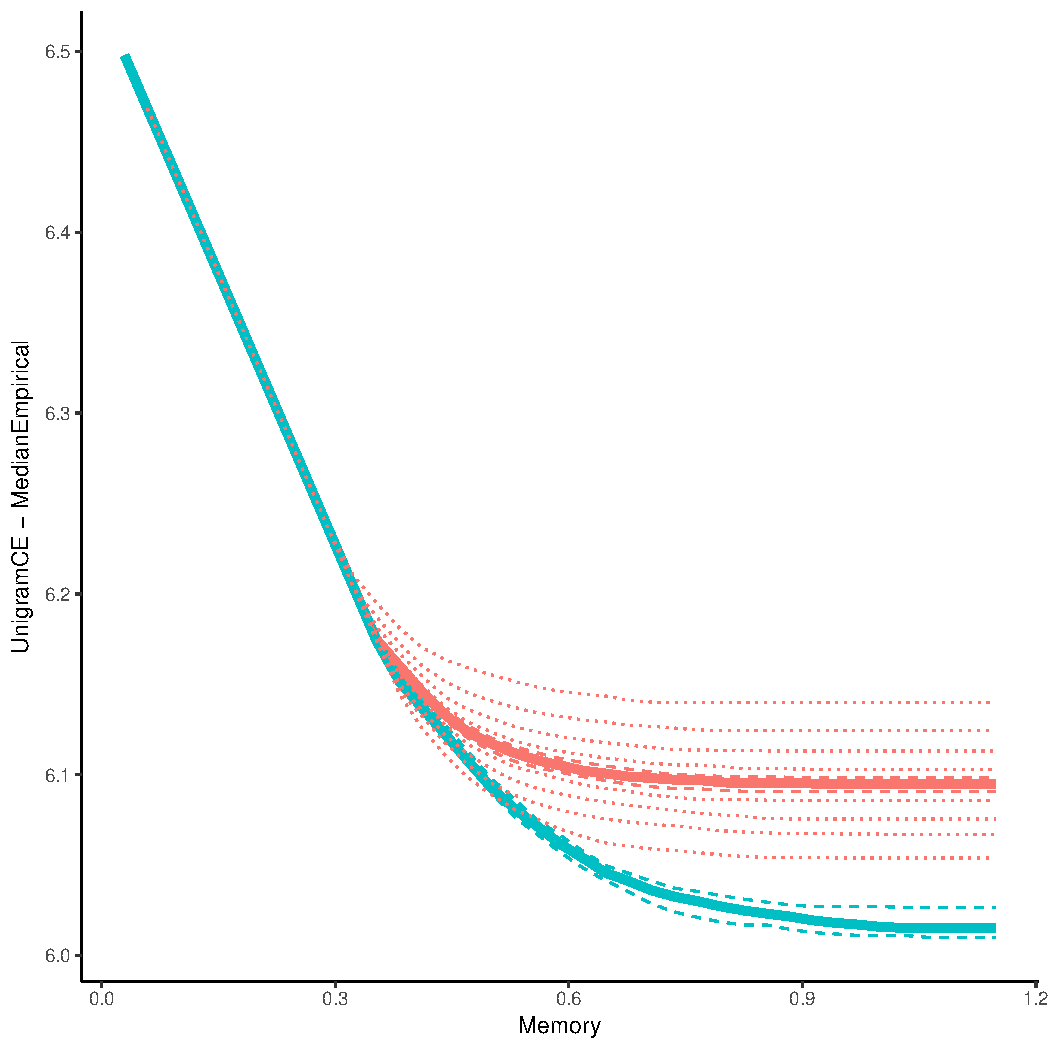
\includegraphics[width=0.25\textwidth]{neural/figures/Kurmanji-Adap-listener-surprisal-memory-MEDIANS_QUANTILES_onlyWordForms_boundedVocab_REAL.pdf} & 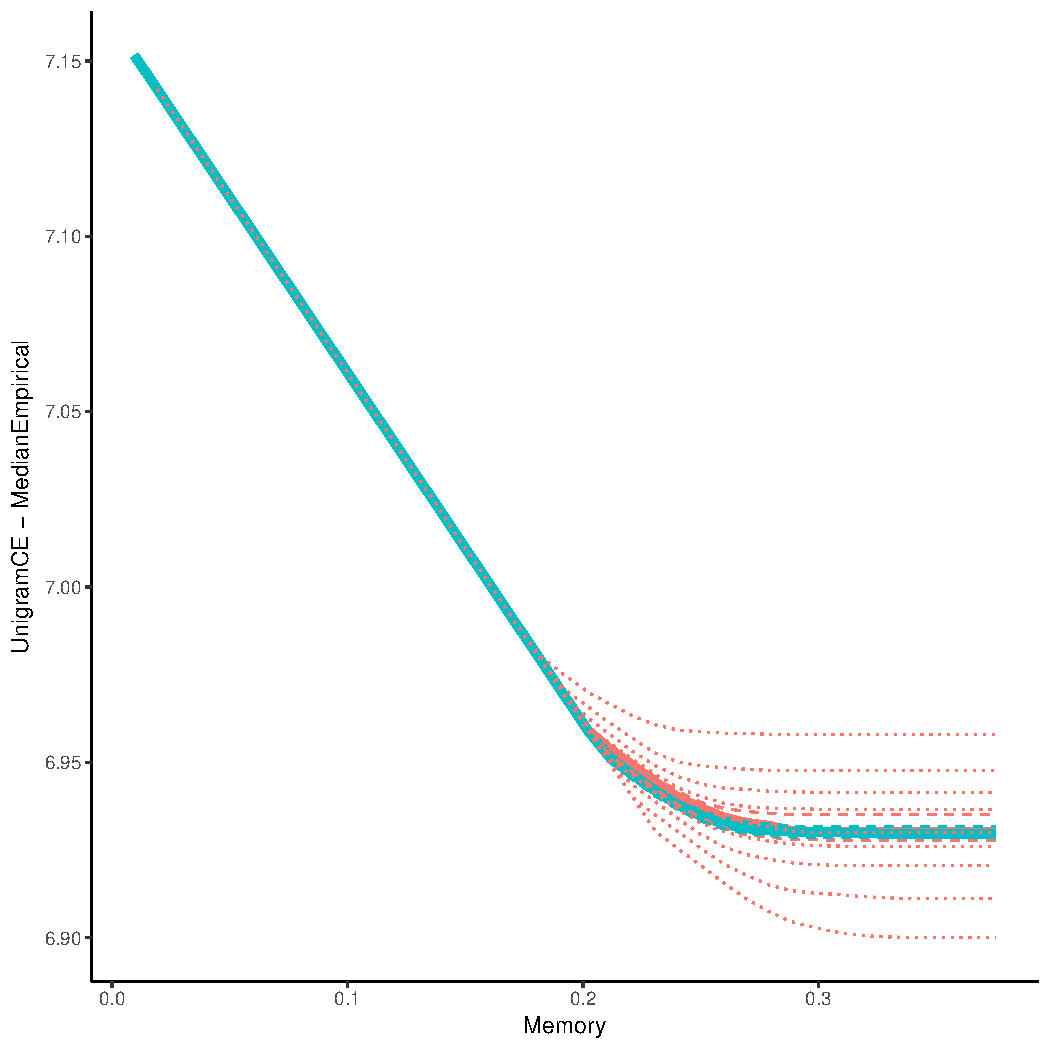
\includegraphics[width=0.25\textwidth]{neural/figures/Latvian-listener-surprisal-memory-MEDIANS_QUANTILES_onlyWordForms_boundedVocab_REAL.pdf} & 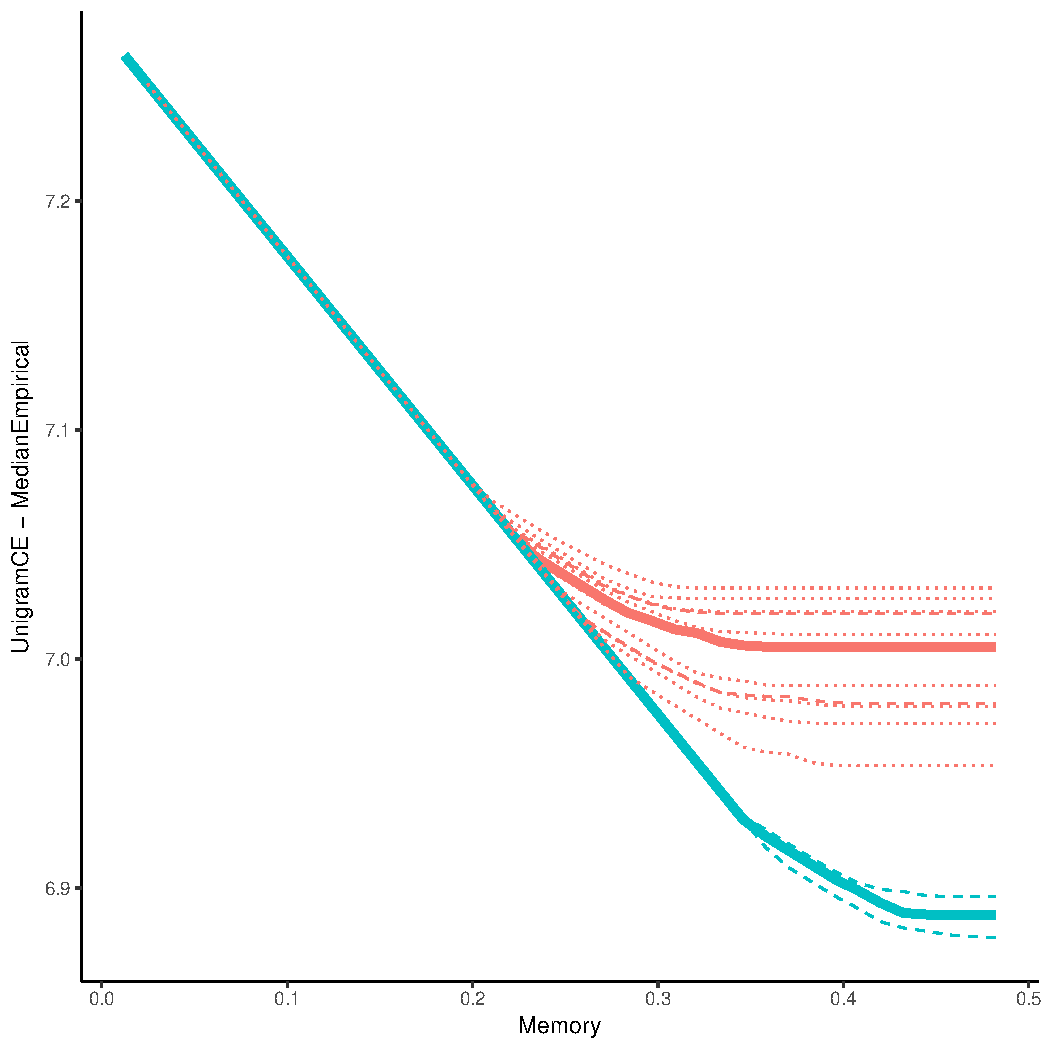
\includegraphics[width=0.25\textwidth]{neural/figures/Maltese-listener-surprisal-memory-MEDIANS_QUANTILES_onlyWordForms_boundedVocab_REAL.pdf} & 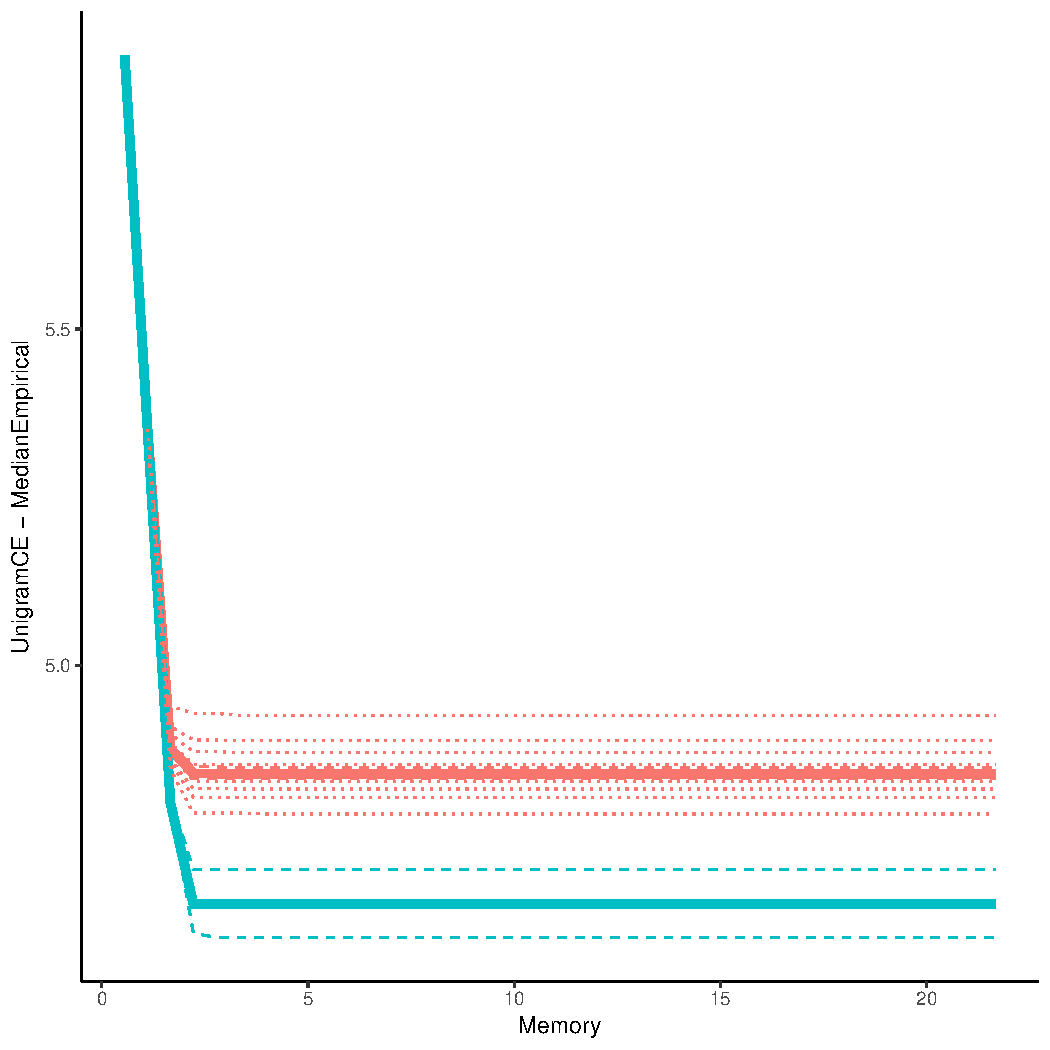
\includegraphics[width=0.25\textwidth]{neural/figures/Naija-Adap-listener-surprisal-memory-MEDIANS_QUANTILES_onlyWordForms_boundedVocab_REAL.pdf}
 \\ 
North Sami & Norwegian & Persian & Polish
 \\ 
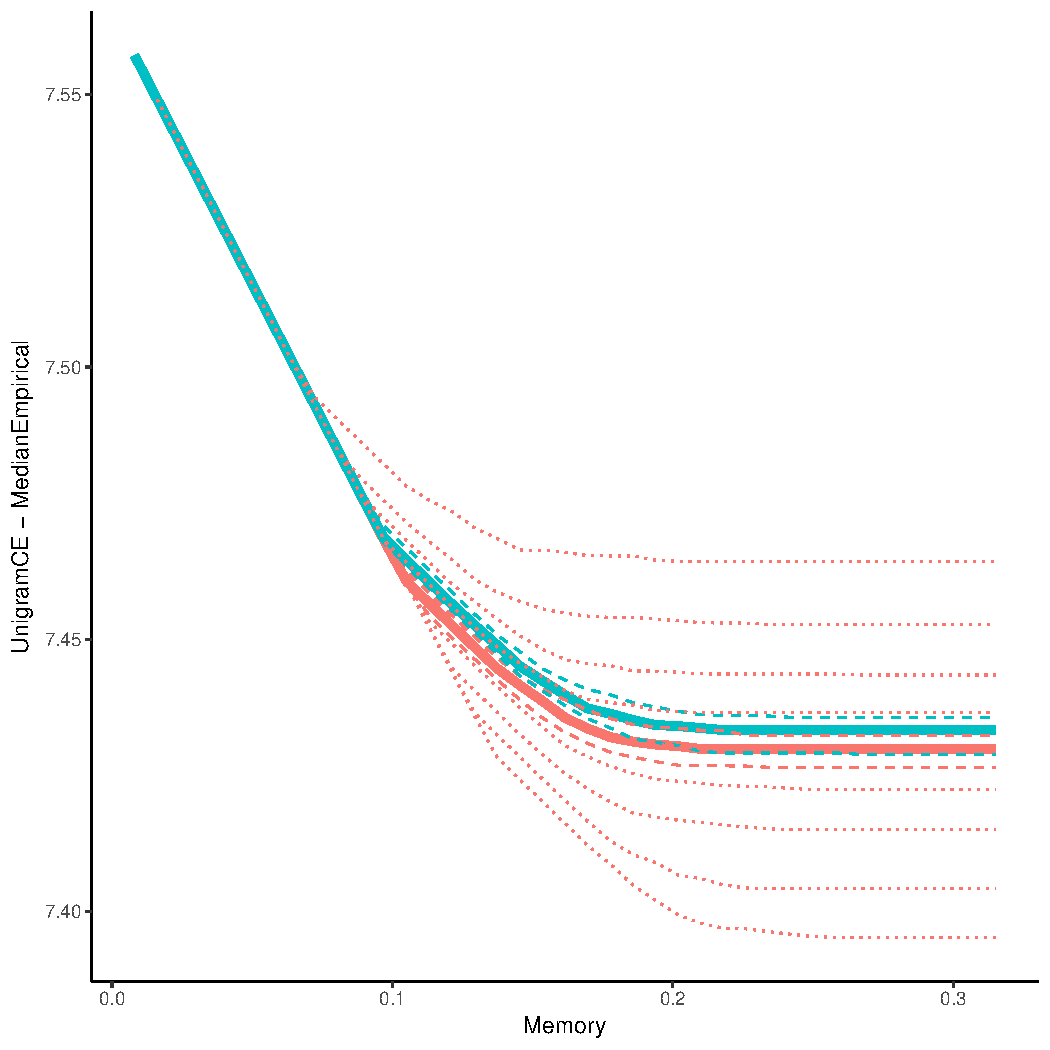
\includegraphics[width=0.25\textwidth]{neural/figures/North_Sami-listener-surprisal-memory-MEDIANS_QUANTILES_onlyWordForms_boundedVocab_REAL.pdf} & 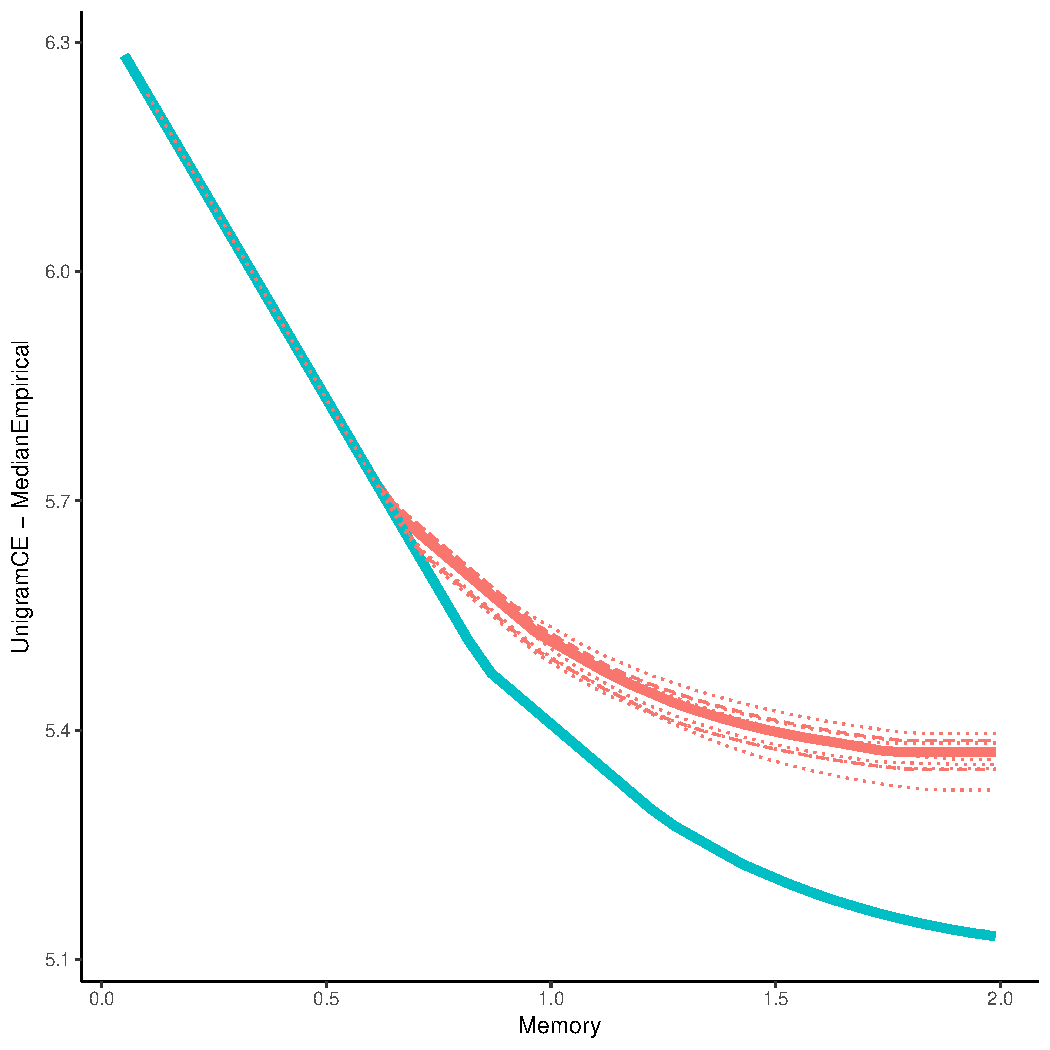
\includegraphics[width=0.25\textwidth]{neural/figures/Norwegian-listener-surprisal-memory-MEDIANS_QUANTILES_onlyWordForms_boundedVocab_REAL.pdf} & 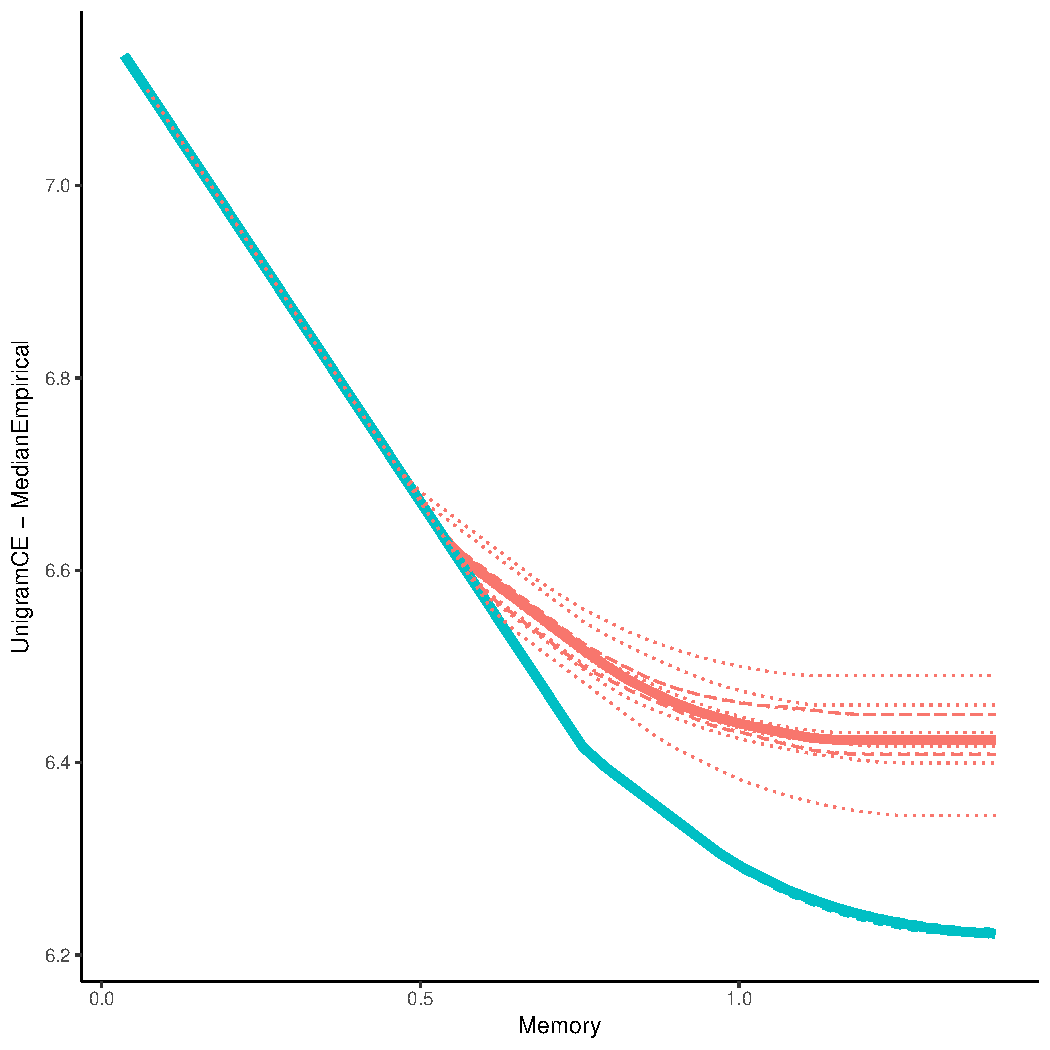
\includegraphics[width=0.25\textwidth]{neural/figures/Persian-listener-surprisal-memory-MEDIANS_QUANTILES_onlyWordForms_boundedVocab_REAL.pdf} & 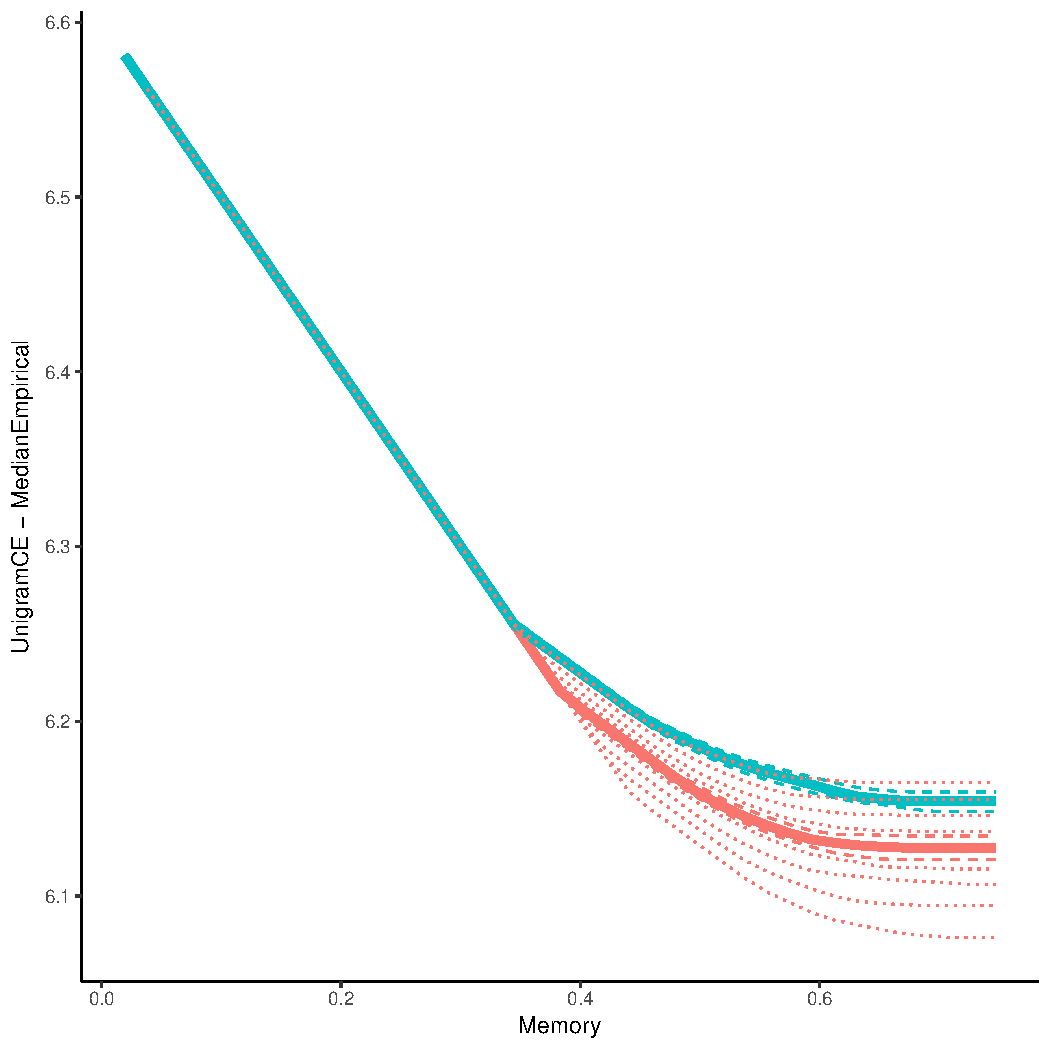
\includegraphics[width=0.25\textwidth]{neural/figures/Polish-listener-surprisal-memory-MEDIANS_QUANTILES_onlyWordForms_boundedVocab_REAL.pdf}
 \\ 
Portuguese & Romanian & Russian & Serbian
 \\ 
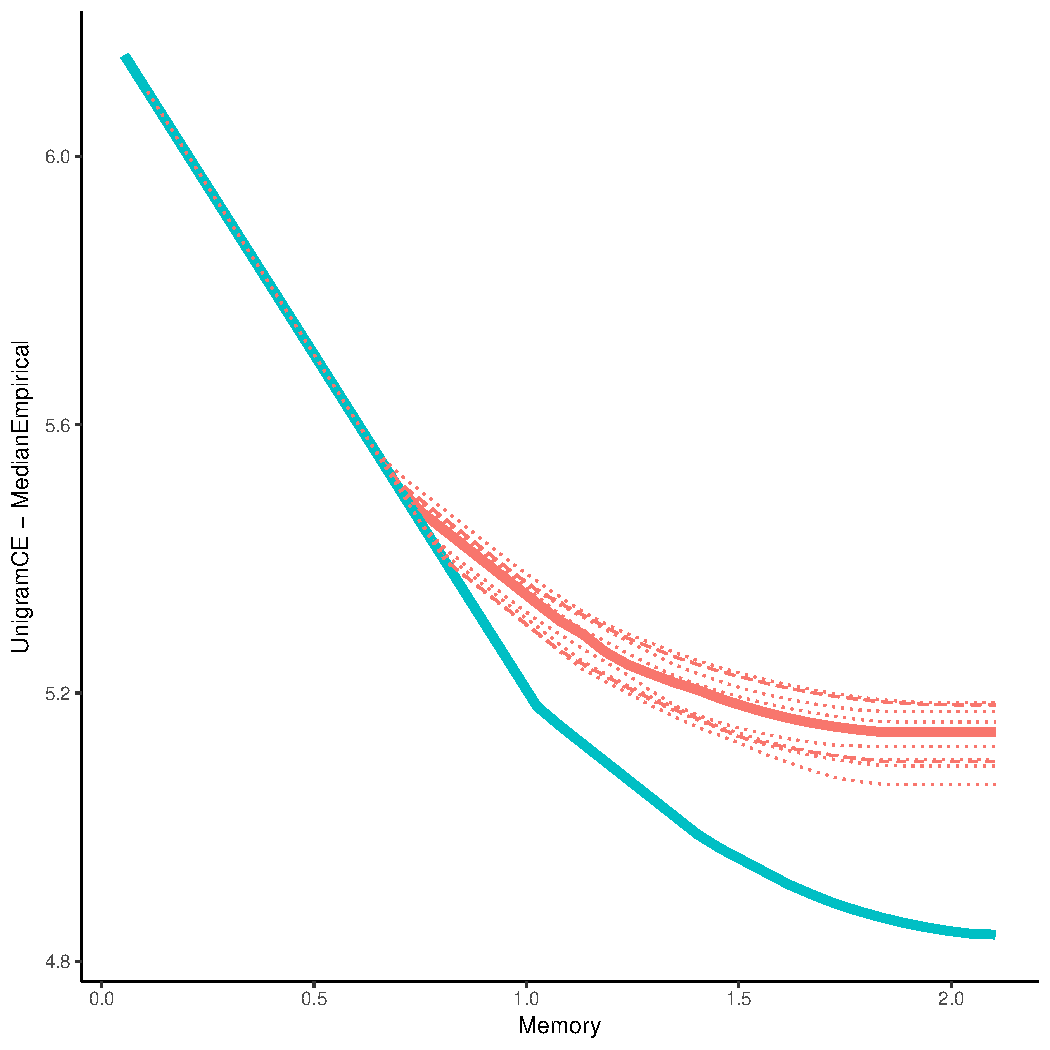
\includegraphics[width=0.25\textwidth]{neural/figures/Portuguese-listener-surprisal-memory-MEDIANS_QUANTILES_onlyWordForms_boundedVocab_REAL.pdf} & 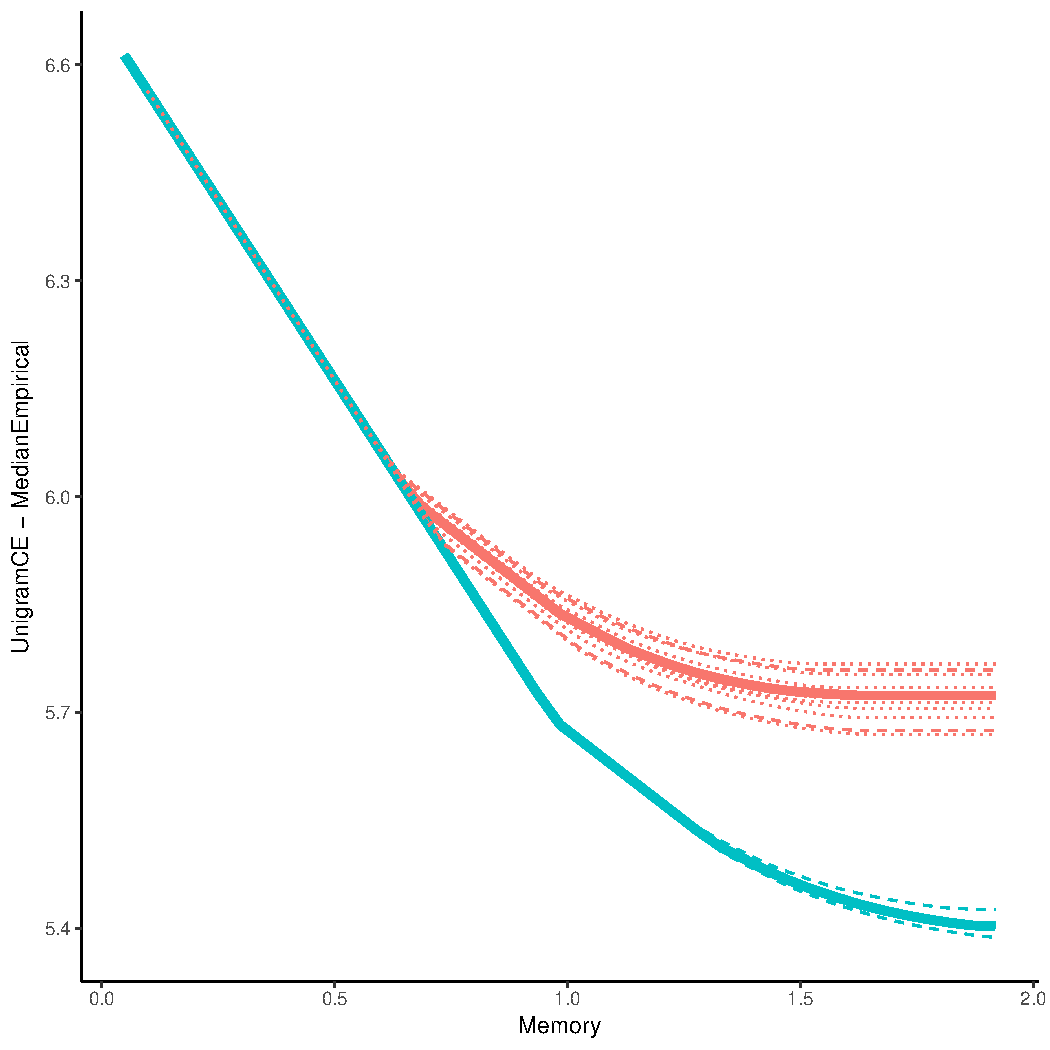
\includegraphics[width=0.25\textwidth]{neural/figures/Romanian-listener-surprisal-memory-MEDIANS_QUANTILES_onlyWordForms_boundedVocab_REAL.pdf} & 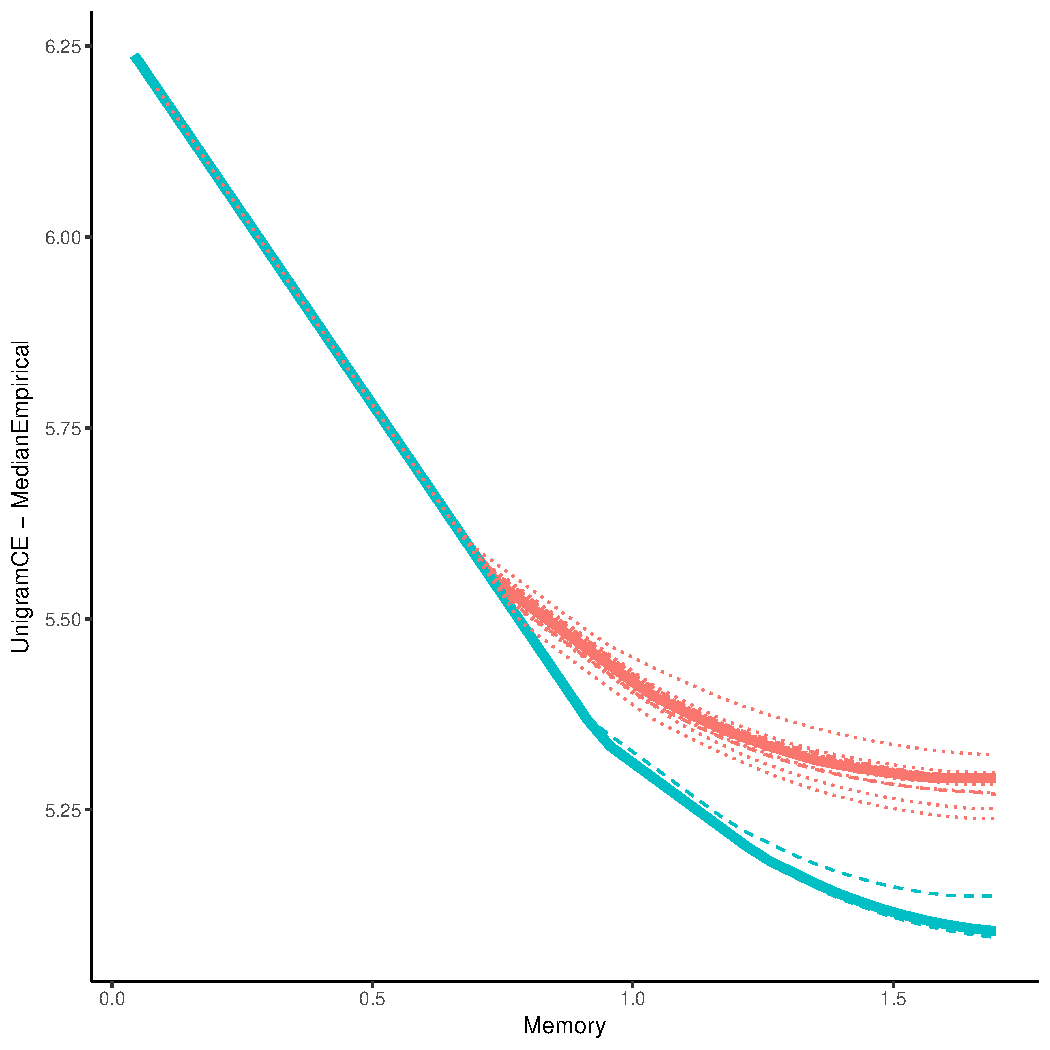
\includegraphics[width=0.25\textwidth]{neural/figures/Russian-listener-surprisal-memory-MEDIANS_QUANTILES_onlyWordForms_boundedVocab_REAL.pdf} & 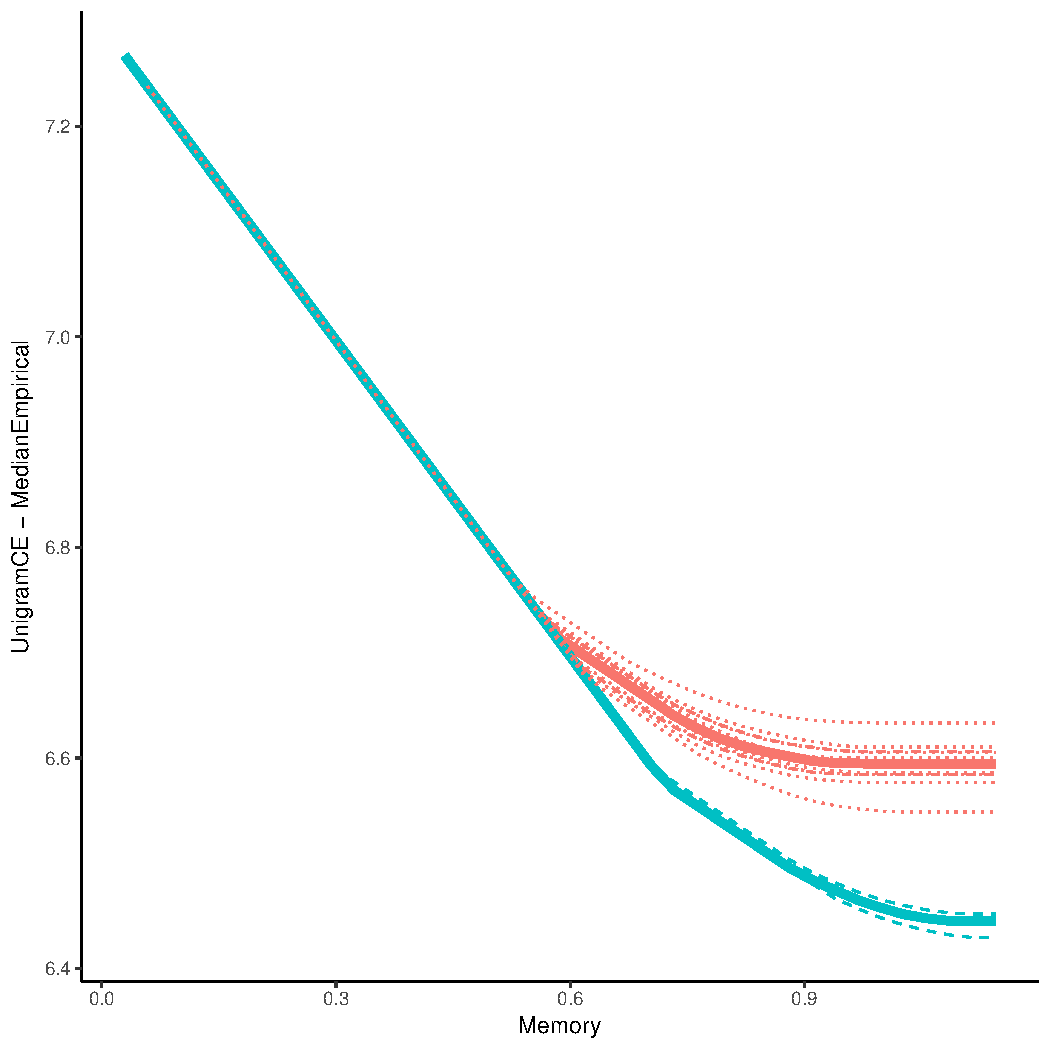
\includegraphics[width=0.25\textwidth]{neural/figures/Serbian-listener-surprisal-memory-MEDIANS_QUANTILES_onlyWordForms_boundedVocab_REAL.pdf}
 \\ 
Slovak & Slovenian & Spanish & Swedish
 \\ 
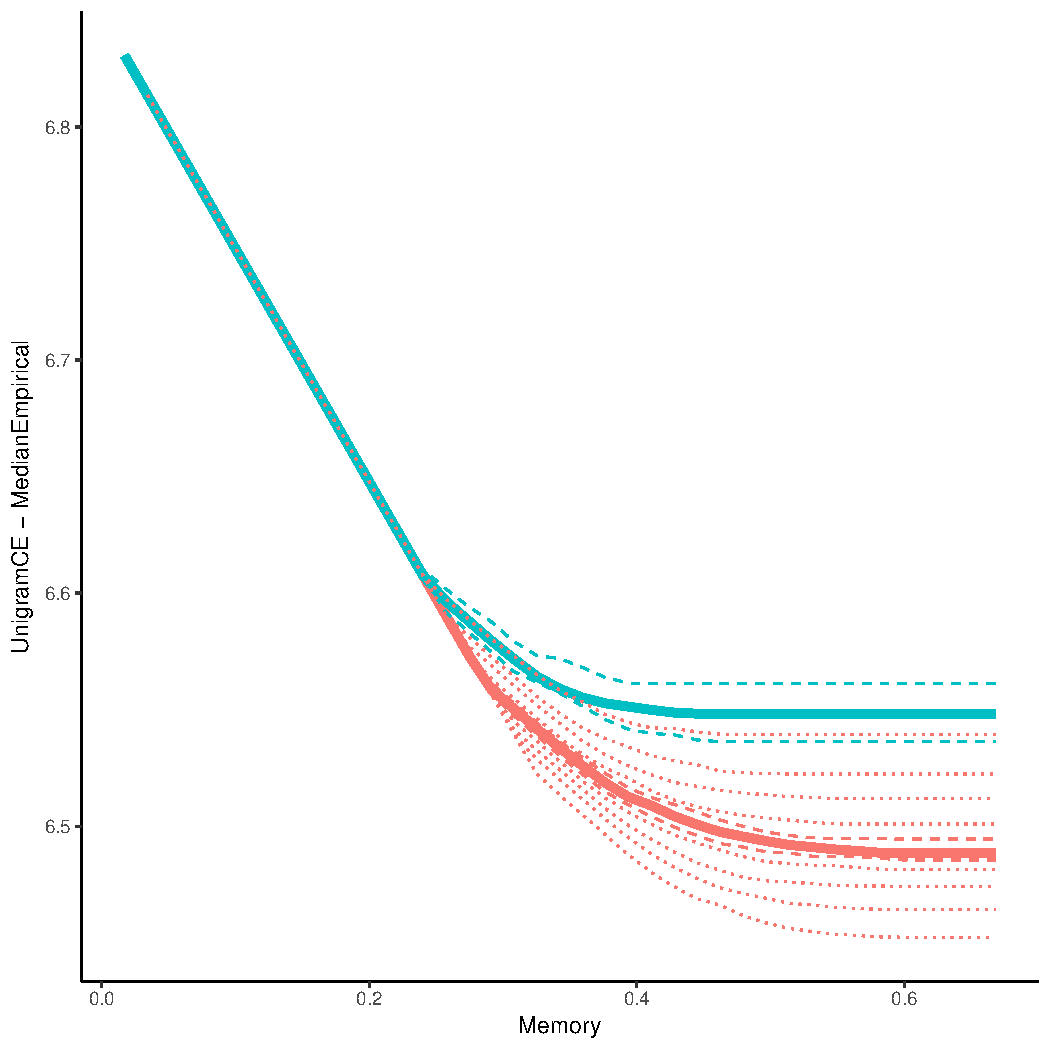
\includegraphics[width=0.25\textwidth]{neural/figures/Slovak-listener-surprisal-memory-MEDIANS_QUANTILES_onlyWordForms_boundedVocab_REAL.pdf} & 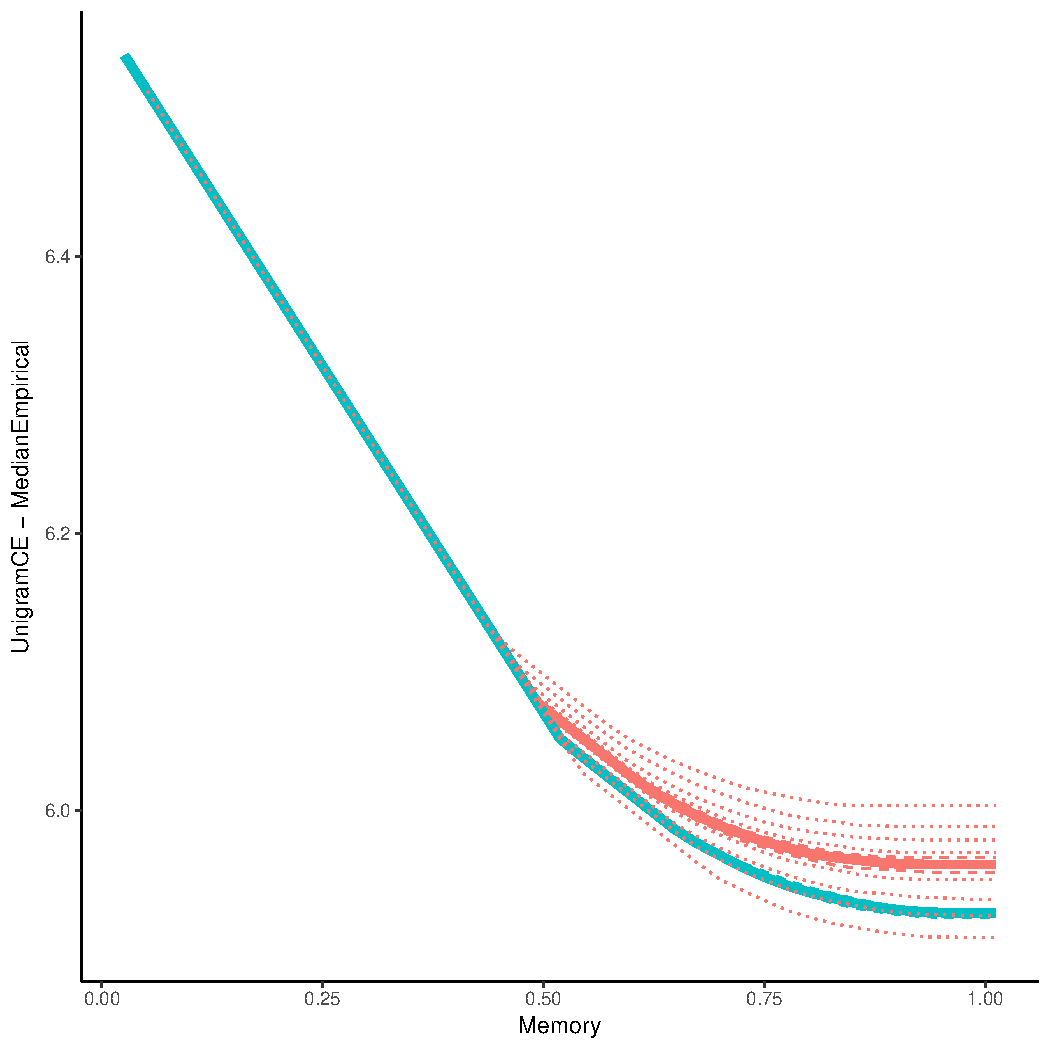
\includegraphics[width=0.25\textwidth]{neural/figures/Slovenian-listener-surprisal-memory-MEDIANS_QUANTILES_onlyWordForms_boundedVocab_REAL.pdf} & 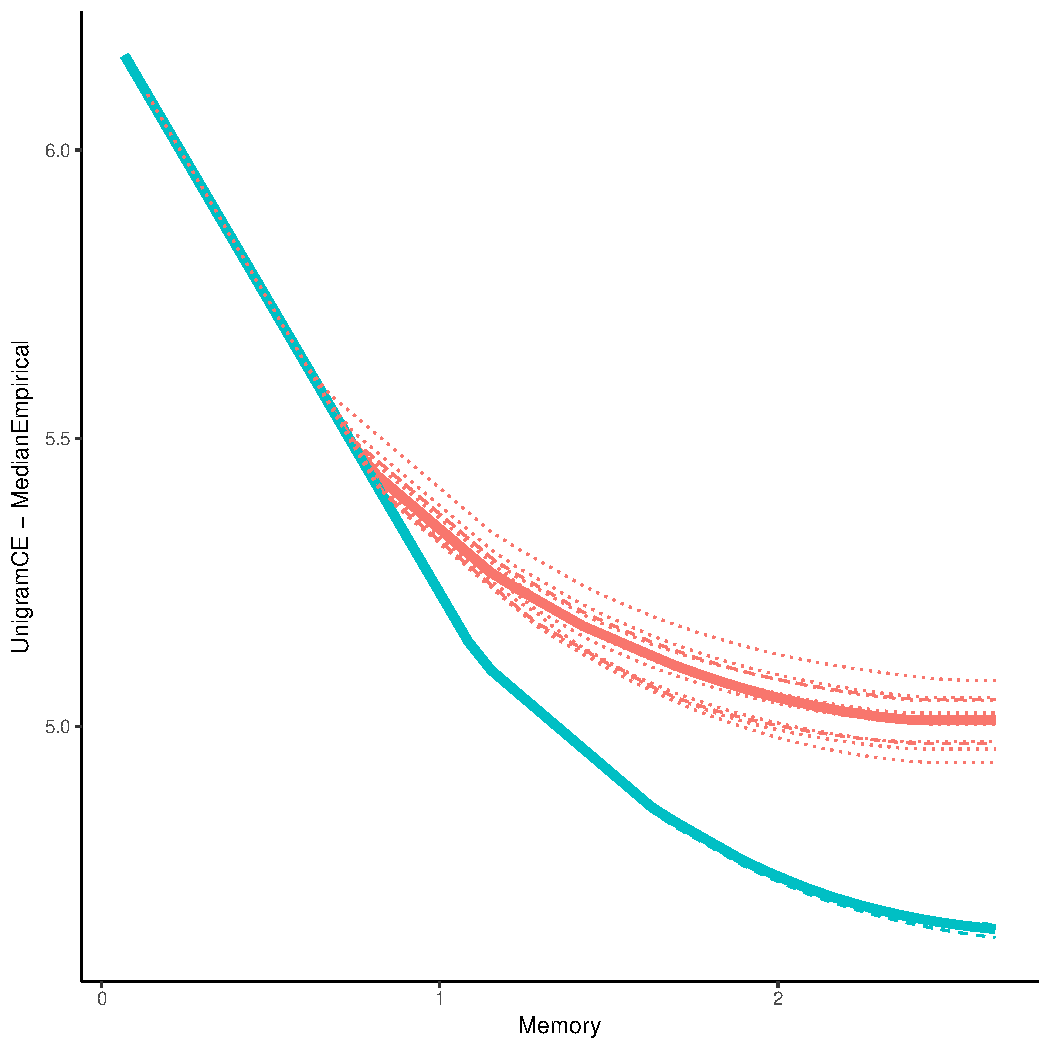
\includegraphics[width=0.25\textwidth]{neural/figures/Spanish-listener-surprisal-memory-MEDIANS_QUANTILES_onlyWordForms_boundedVocab_REAL.pdf} & 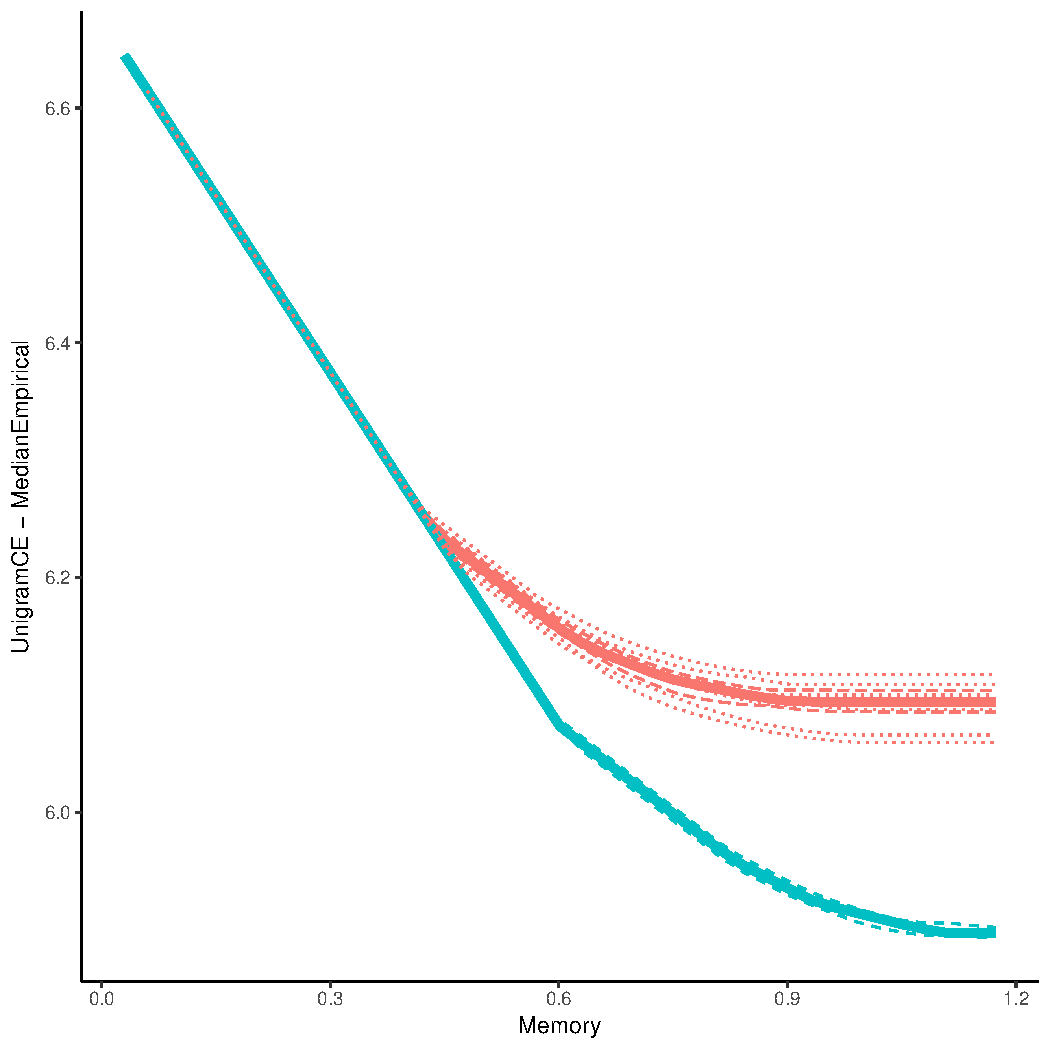
\includegraphics[width=0.25\textwidth]{neural/figures/Swedish-listener-surprisal-memory-MEDIANS_QUANTILES_onlyWordForms_boundedVocab_REAL.pdf}
 \\ 

\end{longtable}
	\captionof{figure}{Medians (cont.)}
\end{center}

\begin{center}
\begin{longtable}{ccccccccccccccclll}
Thai & Turkish & Ukrainian & Urdu
 \\ 
\includegraphics[width=0.25\textwidth]{neural/figures/Thai-Adap-listener-surprisal-memory-MEDIANS_onlyWordForms_boundedVocab_REAL.pdf} & \includegraphics[width=0.25\textwidth]{neural/figures/Turkish-listener-surprisal-memory-MEDIANS_onlyWordForms_boundedVocab_REAL.pdf} & \includegraphics[width=0.25\textwidth]{neural/figures/Ukrainian-listener-surprisal-memory-MEDIANS_onlyWordForms_boundedVocab_REAL.pdf} & \includegraphics[width=0.25\textwidth]{neural/figures/Urdu-listener-surprisal-memory-MEDIANS_onlyWordForms_boundedVocab_REAL.pdf}
 \\ 
Uyghur & Vietnamese &  & 
 \\ 
\includegraphics[width=0.25\textwidth]{neural/figures/Uyghur-Adap-listener-surprisal-memory-MEDIANS_onlyWordForms_boundedVocab_REAL.pdf} & \includegraphics[width=0.25\textwidth]{neural/figures/Vietnamese-listener-surprisal-memory-MEDIANS_onlyWordForms_boundedVocab_REAL.pdf} &  & 
 \\ 

\end{longtable}
	\captionof{figure}{Medians (cont.)}
\end{center}




\subsection{Surprisal at Maximum Memory}


\begin{center}
\begin{longtable}{ccccccccccccccclll}
Afrikaans & Amharic & Arabic & Armenian
 \\ 
\includegraphics[width=0.25\textwidth]{neural/figures/Afrikaans-listener-surprisal-memory-HIST_byMem_onlyWordForms_boundedVocab_REAL.pdf} & \includegraphics[width=0.25\textwidth]{neural/figures/Amharic-Adap-listener-surprisal-memory-HIST_byMem_onlyWordForms_boundedVocab_REAL.pdf} & \includegraphics[width=0.25\textwidth]{neural/figures/Arabic-listener-surprisal-memory-HIST_byMem_onlyWordForms_boundedVocab_REAL.pdf} & \includegraphics[width=0.25\textwidth]{neural/figures/Armenian-Adap-listener-surprisal-memory-HIST_byMem_onlyWordForms_boundedVocab_REAL.pdf}
 \\ 
Bambara & Basque & Breton & Bulgarian
 \\ 
\includegraphics[width=0.25\textwidth]{neural/figures/Bambara-Adap-listener-surprisal-memory-HIST_byMem_onlyWordForms_boundedVocab_REAL.pdf} & \includegraphics[width=0.25\textwidth]{neural/figures/Basque-listener-surprisal-memory-HIST_byMem_onlyWordForms_boundedVocab_REAL.pdf} & \includegraphics[width=0.25\textwidth]{neural/figures/Breton-Adap-listener-surprisal-memory-HIST_byMem_onlyWordForms_boundedVocab_REAL.pdf} & \includegraphics[width=0.25\textwidth]{neural/figures/Bulgarian-listener-surprisal-memory-HIST_byMem_onlyWordForms_boundedVocab_REAL.pdf}
 \\ 
Buryat & Cantonese & Catalan & Chinese
 \\ 
\includegraphics[width=0.25\textwidth]{neural/figures/Buryat-Adap-listener-surprisal-memory-HIST_byMem_onlyWordForms_boundedVocab_REAL.pdf} & \includegraphics[width=0.25\textwidth]{neural/figures/Cantonese-Adap-listener-surprisal-memory-HIST_byMem_onlyWordForms_boundedVocab_REAL.pdf} & \includegraphics[width=0.25\textwidth]{neural/figures/Catalan-listener-surprisal-memory-HIST_byMem_onlyWordForms_boundedVocab_REAL.pdf} & \includegraphics[width=0.25\textwidth]{neural/figures/Chinese-listener-surprisal-memory-HIST_byMem_onlyWordForms_boundedVocab_REAL.pdf}
 \\ 
Croatian & Czech & Danish & Dutch
 \\ 
\includegraphics[width=0.25\textwidth]{neural/figures/Croatian-listener-surprisal-memory-HIST_byMem_onlyWordForms_boundedVocab_REAL.pdf} & \includegraphics[width=0.25\textwidth]{neural/figures/Czech-listener-surprisal-memory-HIST_byMem_onlyWordForms_boundedVocab_REAL.pdf} & \includegraphics[width=0.25\textwidth]{neural/figures/Danish-listener-surprisal-memory-HIST_byMem_onlyWordForms_boundedVocab_REAL.pdf} & \includegraphics[width=0.25\textwidth]{neural/figures/Dutch-listener-surprisal-memory-HIST_byMem_onlyWordForms_boundedVocab_REAL.pdf}
 \\ 

English & Erzya & Estonian & Faroese
 \\ 
\includegraphics[width=0.25\textwidth]{neural/figures/English-listener-surprisal-memory-HIST_byMem_onlyWordForms_boundedVocab_REAL.pdf} & \includegraphics[width=0.25\textwidth]{neural/figures/Erzya-Adap-listener-surprisal-memory-HIST_byMem_onlyWordForms_boundedVocab_REAL.pdf} & \includegraphics[width=0.25\textwidth]{neural/figures/Estonian-listener-surprisal-memory-HIST_byMem_onlyWordForms_boundedVocab_REAL.pdf} & \includegraphics[width=0.25\textwidth]{neural/figures/Faroese-Adap-listener-surprisal-memory-HIST_byMem_onlyWordForms_boundedVocab_REAL.pdf}
 \\ 
Finnish & French & German & Greek
 \\ 
\includegraphics[width=0.25\textwidth]{neural/figures/Finnish-listener-surprisal-memory-HIST_byMem_onlyWordForms_boundedVocab_REAL.pdf} & \includegraphics[width=0.25\textwidth]{neural/figures/French-listener-surprisal-memory-HIST_byMem_onlyWordForms_boundedVocab_REAL.pdf} & \includegraphics[width=0.25\textwidth]{neural/figures/German-listener-surprisal-memory-HIST_byMem_onlyWordForms_boundedVocab_REAL.pdf} & \includegraphics[width=0.25\textwidth]{neural/figures/Greek-listener-surprisal-memory-HIST_byMem_onlyWordForms_boundedVocab_REAL.pdf}
 \\ 
Hebrew & Hindi & Hungarian & Indonesian
 \\ 
\includegraphics[width=0.25\textwidth]{neural/figures/Hebrew-listener-surprisal-memory-HIST_byMem_onlyWordForms_boundedVocab_REAL.pdf} & \includegraphics[width=0.25\textwidth]{neural/figures/Hindi-listener-surprisal-memory-HIST_byMem_onlyWordForms_boundedVocab_REAL.pdf} & \includegraphics[width=0.25\textwidth]{neural/figures/Hungarian-listener-surprisal-memory-HIST_byMem_onlyWordForms_boundedVocab_REAL.pdf} & \includegraphics[width=0.25\textwidth]{neural/figures/Indonesian-listener-surprisal-memory-HIST_byMem_onlyWordForms_boundedVocab_REAL.pdf}
 \\ 
Italian & Japanese & Kazakh & Korean
 \\ 
\includegraphics[width=0.25\textwidth]{neural/figures/Italian-listener-surprisal-memory-HIST_byMem_onlyWordForms_boundedVocab_REAL.pdf} & \includegraphics[width=0.25\textwidth]{neural/figures/Japanese-listener-surprisal-memory-HIST_byMem_onlyWordForms_boundedVocab_REAL.pdf} & \includegraphics[width=0.25\textwidth]{neural/figures/Kazakh-Adap-listener-surprisal-memory-HIST_byMem_onlyWordForms_boundedVocab_REAL.pdf} & \includegraphics[width=0.25\textwidth]{neural/figures/Korean-listener-surprisal-memory-HIST_byMem_onlyWordForms_boundedVocab_REAL.pdf}
 \\ 

Kurmanji & Latvian & Maltese & Naija
 \\ 
\includegraphics[width=0.25\textwidth]{neural/figures/Kurmanji-Adap-listener-surprisal-memory-HIST_byMem_onlyWordForms_boundedVocab_REAL.pdf} & \includegraphics[width=0.25\textwidth]{neural/figures/Latvian-listener-surprisal-memory-HIST_byMem_onlyWordForms_boundedVocab_REAL.pdf} & \includegraphics[width=0.25\textwidth]{neural/figures/Maltese-listener-surprisal-memory-HIST_byMem_onlyWordForms_boundedVocab_REAL.pdf} & \includegraphics[width=0.25\textwidth]{neural/figures/Naija-Adap-listener-surprisal-memory-HIST_byMem_onlyWordForms_boundedVocab_REAL.pdf}
 \\ 
North Sami & Norwegian & Persian & Polish
 \\ 
\includegraphics[width=0.25\textwidth]{neural/figures/North_Sami-listener-surprisal-memory-HIST_byMem_onlyWordForms_boundedVocab_REAL.pdf} & \includegraphics[width=0.25\textwidth]{neural/figures/Norwegian-listener-surprisal-memory-HIST_byMem_onlyWordForms_boundedVocab_REAL.pdf} & \includegraphics[width=0.25\textwidth]{neural/figures/Persian-listener-surprisal-memory-HIST_byMem_onlyWordForms_boundedVocab_REAL.pdf} & \includegraphics[width=0.25\textwidth]{neural/figures/Polish-listener-surprisal-memory-HIST_byMem_onlyWordForms_boundedVocab_REAL.pdf}
 \\ 
Portuguese & Romanian & Russian & Serbian
 \\ 
\includegraphics[width=0.25\textwidth]{neural/figures/Portuguese-listener-surprisal-memory-HIST_byMem_onlyWordForms_boundedVocab_REAL.pdf} & \includegraphics[width=0.25\textwidth]{neural/figures/Romanian-listener-surprisal-memory-HIST_byMem_onlyWordForms_boundedVocab_REAL.pdf} & \includegraphics[width=0.25\textwidth]{neural/figures/Russian-listener-surprisal-memory-HIST_byMem_onlyWordForms_boundedVocab_REAL.pdf} & \includegraphics[width=0.25\textwidth]{neural/figures/Serbian-listener-surprisal-memory-HIST_byMem_onlyWordForms_boundedVocab_REAL.pdf}
 \\ 
Slovak & Slovenian & Spanish & Swedish
 \\ 
\includegraphics[width=0.25\textwidth]{neural/figures/Slovak-listener-surprisal-memory-HIST_byMem_onlyWordForms_boundedVocab_REAL.pdf} & \includegraphics[width=0.25\textwidth]{neural/figures/Slovenian-listener-surprisal-memory-HIST_byMem_onlyWordForms_boundedVocab_REAL.pdf} & \includegraphics[width=0.25\textwidth]{neural/figures/Spanish-listener-surprisal-memory-HIST_byMem_onlyWordForms_boundedVocab_REAL.pdf} & \includegraphics[width=0.25\textwidth]{neural/figures/Swedish-listener-surprisal-memory-HIST_byMem_onlyWordForms_boundedVocab_REAL.pdf}
 \\ 

Thai & Turkish & Ukrainian & Urdu
 \\ 
\includegraphics[width=0.25\textwidth]{neural/figures/Thai-Adap-listener-surprisal-memory-HIST_byMem_onlyWordForms_boundedVocab_REAL.pdf} & \includegraphics[width=0.25\textwidth]{neural/figures/Turkish-listener-surprisal-memory-HIST_byMem_onlyWordForms_boundedVocab_REAL.pdf} & \includegraphics[width=0.25\textwidth]{neural/figures/Ukrainian-listener-surprisal-memory-HIST_byMem_onlyWordForms_boundedVocab_REAL.pdf} & \includegraphics[width=0.25\textwidth]{neural/figures/Urdu-listener-surprisal-memory-HIST_byMem_onlyWordForms_boundedVocab_REAL.pdf}
 \\ 
Uyghur & Vietnamese &  & 
 \\ 
\includegraphics[width=0.25\textwidth]{neural/figures/Uyghur-Adap-listener-surprisal-memory-HIST_byMem_onlyWordForms_boundedVocab_REAL.pdf} & \includegraphics[width=0.25\textwidth]{neural/figures/Vietnamese-listener-surprisal-memory-HIST_byMem_onlyWordForms_boundedVocab_REAL.pdf} &  & 
 \\ 

\end{longtable}
	\captionof{figure}{Histograms: Surprisal, at maximum memory.}\label{tab:slice-hists-real}
\end{center}


%\begin{table}
%\begin{tabular}{cccccccccccccccccc}
%Afrikaans & Amharic & Arabic & Armenian
 \\ 
\includegraphics[width=0.25\textwidth]{neural/figures/Afrikaans-listener-surprisal-memory-QUANTILES_onlyWordForms_boundedVocab_REAL.pdf} & \includegraphics[width=0.25\textwidth]{neural/figures/Amharic-Adap-listener-surprisal-memory-QUANTILES_onlyWordForms_boundedVocab_REAL.pdf} & \includegraphics[width=0.25\textwidth]{neural/figures/Arabic-listener-surprisal-memory-QUANTILES_onlyWordForms_boundedVocab_REAL.pdf} & \includegraphics[width=0.25\textwidth]{neural/figures/Armenian-Adap-listener-surprisal-memory-QUANTILES_onlyWordForms_boundedVocab_REAL.pdf}
 \\ 
Bambara & Basque & Breton & Bulgarian
 \\ 
\includegraphics[width=0.25\textwidth]{neural/figures/Bambara-Adap-listener-surprisal-memory-QUANTILES_onlyWordForms_boundedVocab_REAL.pdf} & \includegraphics[width=0.25\textwidth]{neural/figures/Basque-listener-surprisal-memory-QUANTILES_onlyWordForms_boundedVocab_REAL.pdf} & \includegraphics[width=0.25\textwidth]{neural/figures/Breton-Adap-listener-surprisal-memory-QUANTILES_onlyWordForms_boundedVocab_REAL.pdf} & \includegraphics[width=0.25\textwidth]{neural/figures/Bulgarian-listener-surprisal-memory-QUANTILES_onlyWordForms_boundedVocab_REAL.pdf}
 \\ 
Buryat & Cantonese & Catalan & Chinese
 \\ 
\includegraphics[width=0.25\textwidth]{neural/figures/Buryat-Adap-listener-surprisal-memory-QUANTILES_onlyWordForms_boundedVocab_REAL.pdf} & \includegraphics[width=0.25\textwidth]{neural/figures/Cantonese-Adap-listener-surprisal-memory-QUANTILES_onlyWordForms_boundedVocab_REAL.pdf} & \includegraphics[width=0.25\textwidth]{neural/figures/Catalan-listener-surprisal-memory-QUANTILES_onlyWordForms_boundedVocab_REAL.pdf} & \includegraphics[width=0.25\textwidth]{neural/figures/Chinese-listener-surprisal-memory-QUANTILES_onlyWordForms_boundedVocab_REAL.pdf}
 \\ 
Croatian & Czech & Danish & Dutch
 \\ 
\includegraphics[width=0.25\textwidth]{neural/figures/Croatian-listener-surprisal-memory-QUANTILES_onlyWordForms_boundedVocab_REAL.pdf} & \includegraphics[width=0.25\textwidth]{neural/figures/Czech-listener-surprisal-memory-QUANTILES_onlyWordForms_boundedVocab_REAL.pdf} & \includegraphics[width=0.25\textwidth]{neural/figures/Danish-listener-surprisal-memory-QUANTILES_onlyWordForms_boundedVocab_REAL.pdf} & \includegraphics[width=0.25\textwidth]{neural/figures/Dutch-listener-surprisal-memory-QUANTILES_onlyWordForms_boundedVocab_REAL.pdf}
 \\ 
English & Erzya & Estonian & Faroese
 \\ 
\includegraphics[width=0.25\textwidth]{neural/figures/English-listener-surprisal-memory-QUANTILES_onlyWordForms_boundedVocab_REAL.pdf} & \includegraphics[width=0.25\textwidth]{neural/figures/Erzya-Adap-listener-surprisal-memory-QUANTILES_onlyWordForms_boundedVocab_REAL.pdf} & \includegraphics[width=0.25\textwidth]{neural/figures/Estonian-listener-surprisal-memory-QUANTILES_onlyWordForms_boundedVocab_REAL.pdf} & \includegraphics[width=0.25\textwidth]{neural/figures/Faroese-Adap-listener-surprisal-memory-QUANTILES_onlyWordForms_boundedVocab_REAL.pdf}
 \\ 

%\end{tabular}
%	\captionof{figure}{Quantiles: At a given memory budget, what percentage of the baselines results in higher listener surprisal than the real language? Solid curves represent sample means, dashed lines represent 95 \% confidence bounds; dotted lines represent 99.9 \% confidence bounds. At five evenly spaced memory levels, we provide a p-value for the null hypothesis that the actual population mean is $0.5$ or less. Confidence bounds and p-values are obtained using an exact nonparametric method (see text).}\label{tab:quantiles}
%\end{center}
%
%\begin{table}
%\begin{tabular}{cccccccccccccccccc}
%Finnish & French & German & Greek
 \\ 
\includegraphics[width=0.25\textwidth]{neural/figures/Finnish-listener-surprisal-memory-QUANTILES_onlyWordForms_boundedVocab_REAL.pdf} & \includegraphics[width=0.25\textwidth]{neural/figures/French-listener-surprisal-memory-QUANTILES_onlyWordForms_boundedVocab_REAL.pdf} & \includegraphics[width=0.25\textwidth]{neural/figures/German-listener-surprisal-memory-QUANTILES_onlyWordForms_boundedVocab_REAL.pdf} & \includegraphics[width=0.25\textwidth]{neural/figures/Greek-listener-surprisal-memory-QUANTILES_onlyWordForms_boundedVocab_REAL.pdf}
 \\ 
Hebrew & Hindi & Hungarian & Indonesian
 \\ 
\includegraphics[width=0.25\textwidth]{neural/figures/Hebrew-listener-surprisal-memory-QUANTILES_onlyWordForms_boundedVocab_REAL.pdf} & \includegraphics[width=0.25\textwidth]{neural/figures/Hindi-listener-surprisal-memory-QUANTILES_onlyWordForms_boundedVocab_REAL.pdf} & \includegraphics[width=0.25\textwidth]{neural/figures/Hungarian-listener-surprisal-memory-QUANTILES_onlyWordForms_boundedVocab_REAL.pdf} & \includegraphics[width=0.25\textwidth]{neural/figures/Indonesian-listener-surprisal-memory-QUANTILES_onlyWordForms_boundedVocab_REAL.pdf}
 \\ 
Italian & Japanese & Kazakh & Korean
 \\ 
\includegraphics[width=0.25\textwidth]{neural/figures/Italian-listener-surprisal-memory-QUANTILES_onlyWordForms_boundedVocab_REAL.pdf} & \includegraphics[width=0.25\textwidth]{neural/figures/Japanese-listener-surprisal-memory-QUANTILES_onlyWordForms_boundedVocab_REAL.pdf} & \includegraphics[width=0.25\textwidth]{neural/figures/Kazakh-Adap-listener-surprisal-memory-QUANTILES_onlyWordForms_boundedVocab_REAL.pdf} & \includegraphics[width=0.25\textwidth]{neural/figures/Korean-listener-surprisal-memory-QUANTILES_onlyWordForms_boundedVocab_REAL.pdf}
 \\ 
Kurmanji & Latvian & Maltese & Naija
 \\ 
\includegraphics[width=0.25\textwidth]{neural/figures/Kurmanji-Adap-listener-surprisal-memory-QUANTILES_onlyWordForms_boundedVocab_REAL.pdf} & \includegraphics[width=0.25\textwidth]{neural/figures/Latvian-listener-surprisal-memory-QUANTILES_onlyWordForms_boundedVocab_REAL.pdf} & \includegraphics[width=0.25\textwidth]{neural/figures/Maltese-listener-surprisal-memory-QUANTILES_onlyWordForms_boundedVocab_REAL.pdf} & \includegraphics[width=0.25\textwidth]{neural/figures/Naija-Adap-listener-surprisal-memory-QUANTILES_onlyWordForms_boundedVocab_REAL.pdf}
 \\ 
North Sami & Norwegian & Persian & Polish
 \\ 
\includegraphics[width=0.25\textwidth]{neural/figures/North_Sami-listener-surprisal-memory-QUANTILES_onlyWordForms_boundedVocab_REAL.pdf} & \includegraphics[width=0.25\textwidth]{neural/figures/Norwegian-listener-surprisal-memory-QUANTILES_onlyWordForms_boundedVocab_REAL.pdf} & \includegraphics[width=0.25\textwidth]{neural/figures/Persian-listener-surprisal-memory-QUANTILES_onlyWordForms_boundedVocab_REAL.pdf} & \includegraphics[width=0.25\textwidth]{neural/figures/Polish-listener-surprisal-memory-QUANTILES_onlyWordForms_boundedVocab_REAL.pdf}
 \\ 

%\end{tabular}
%	\captionof{figure}{Quantiles (part 2)}
%\end{center}
%
%\begin{table}
%\begin{tabular}{cccccccccccccccccc}
%Portuguese & Romanian & Russian & Serbian
 \\ 
\includegraphics[width=0.25\textwidth]{neural/figures/Portuguese-listener-surprisal-memory-QUANTILES_onlyWordForms_boundedVocab_REAL.pdf} & \includegraphics[width=0.25\textwidth]{neural/figures/Romanian-listener-surprisal-memory-QUANTILES_onlyWordForms_boundedVocab_REAL.pdf} & \includegraphics[width=0.25\textwidth]{neural/figures/Russian-listener-surprisal-memory-QUANTILES_onlyWordForms_boundedVocab_REAL.pdf} & \includegraphics[width=0.25\textwidth]{neural/figures/Serbian-listener-surprisal-memory-QUANTILES_onlyWordForms_boundedVocab_REAL.pdf}
 \\ 
Slovak & Slovenian & Spanish & Swedish
 \\ 
\includegraphics[width=0.25\textwidth]{neural/figures/Slovak-listener-surprisal-memory-QUANTILES_onlyWordForms_boundedVocab_REAL.pdf} & \includegraphics[width=0.25\textwidth]{neural/figures/Slovenian-listener-surprisal-memory-QUANTILES_onlyWordForms_boundedVocab_REAL.pdf} & \includegraphics[width=0.25\textwidth]{neural/figures/Spanish-listener-surprisal-memory-QUANTILES_onlyWordForms_boundedVocab_REAL.pdf} & \includegraphics[width=0.25\textwidth]{neural/figures/Swedish-listener-surprisal-memory-QUANTILES_onlyWordForms_boundedVocab_REAL.pdf}
 \\ 
Thai & Turkish & Ukrainian & Urdu
 \\ 
\includegraphics[width=0.25\textwidth]{neural/figures/Thai-Adap-listener-surprisal-memory-QUANTILES_onlyWordForms_boundedVocab_REAL.pdf} & \includegraphics[width=0.25\textwidth]{neural/figures/Turkish-listener-surprisal-memory-QUANTILES_onlyWordForms_boundedVocab_REAL.pdf} & \includegraphics[width=0.25\textwidth]{neural/figures/Ukrainian-listener-surprisal-memory-QUANTILES_onlyWordForms_boundedVocab_REAL.pdf} & \includegraphics[width=0.25\textwidth]{neural/figures/Urdu-listener-surprisal-memory-QUANTILES_onlyWordForms_boundedVocab_REAL.pdf}
 \\ 
Uyghur & Vietnamese &  & 
 \\ 
\includegraphics[width=0.25\textwidth]{neural/figures/Uyghur-Adap-listener-surprisal-memory-QUANTILES_onlyWordForms_boundedVocab_REAL.pdf} & \includegraphics[width=0.25\textwidth]{neural/figures/Vietnamese-listener-surprisal-memory-QUANTILES_onlyWordForms_boundedVocab_REAL.pdf} &  & 
 \\ 

%\end{tabular}
%	\captionof{figure}{Quantiles (part 3)}
%\end{center}
%
%
%














\subsection{Samples Drawn (Experiment 3)}



\begin{center}
\begin{tabular}{l|ll||l|llllllllllllll}
	Language & Base. & MLE & Language & Base. & MLE \\ \hline
Afrikaans  &  13  &  10  &  Indonesian  &  11  &  10  \\
Amharic  &  137  &  71  &  Italian  &  10  &  10  \\
Arabic  &  11  &  10  &  Japanese  &  25  &  10  \\
Armenian  &  140  &  17  &  Kazakh  &  11  &  10  \\
Bambara  &  25  &  10  &  Korean  &  11  &  10  \\
Basque  &  15  &  10  &  Kurmanji  &  338  &  101  \\
Breton  &  35  &  10  &  Latvian  &  308  &  132  \\
Bulgarian  &  14  &  10  &  Maltese  &  30  &  10  \\
Buryat  &  26  &  10  &  Naija  &  214  &  93  \\
Cantonese  &  306  &  135  &  North Sami  &  335  &  101  \\
Catalan  &  11  &  10  &  Norwegian  &  12  &  10  \\
Chinese  &  21  &  10  &  Persian  &  25  &  10  \\
Croatian  &  30  &  10  &  Polish  &  309  &  131  \\
Czech  &  18  &  12  &  Portuguese  &  15  &  99  \\
Danish  &  33  &  10  &  Romanian  &  10  &  10  \\
Dutch  &  27  &  10  &  Russian  &  20  &  13  \\
English  &  13  &  10  &  Serbian  &  26  &  11  \\
Erzya  &  846  &  101  &  Slovak  &  303  &  138  \\
Estonian  &  347  &  10  &  Slovenian  &  297  &  12  \\
Faroese  &  27  &  10  &  Spanish  &  14  &  10  \\
Finnish  &  83  &  54  &  Swedish  &  31  &  10  \\
French  &  14  &  12  &  Thai  &  45  &  10  \\
German  &  19  &  10  &  Turkish  &  13  &  10  \\
Greek  &  16  &  10  &  Ukrainian  &  28  &  10  \\
Hebrew  &  11  &  10  &  Urdu  &  17  &  10  \\
Hindi  &  11  &  10  &  Uyghur  &  326  &  132  \\
Hungarian  &  220  &  35  &  Vietnamese  &  303  &  132  \\

\end{tabular}
	\captionof{figure}{Experiment 3: Samples drawn per language according to the precision-dependent stopping criterion.}\label{tab:samples}
\end{center}



\subsection{Medians (Experiment 3)}

\begin{center}
\begin{longtable}{ccccccccccccccclll}
Afrikaans & Amharic & Arabic & Armenian
 \\ 
\includegraphics[width=0.25\textwidth]{neural/figures/Afrikaans-listener-surprisal-memory-MEDIANS_QUANTILES_onlyWordForms_boundedVocab.pdf} & \includegraphics[width=0.25\textwidth]{neural/figures/Amharic-Adap-listener-surprisal-memory-MEDIANS_QUANTILES_onlyWordForms_boundedVocab.pdf} & \includegraphics[width=0.25\textwidth]{neural/figures/Arabic-listener-surprisal-memory-MEDIANS_QUANTILES_onlyWordForms_boundedVocab.pdf} & \includegraphics[width=0.25\textwidth]{neural/figures/Armenian-Adap-listener-surprisal-memory-MEDIANS_QUANTILES_onlyWordForms_boundedVocab.pdf}
 \\ 
Bambara & Basque & Breton & Bulgarian
 \\ 
\includegraphics[width=0.25\textwidth]{neural/figures/Bambara-Adap-listener-surprisal-memory-MEDIANS_QUANTILES_onlyWordForms_boundedVocab.pdf} & \includegraphics[width=0.25\textwidth]{neural/figures/Basque-listener-surprisal-memory-MEDIANS_QUANTILES_onlyWordForms_boundedVocab.pdf} & \includegraphics[width=0.25\textwidth]{neural/figures/Breton-Adap-listener-surprisal-memory-MEDIANS_QUANTILES_onlyWordForms_boundedVocab.pdf} & \includegraphics[width=0.25\textwidth]{neural/figures/Bulgarian-listener-surprisal-memory-MEDIANS_QUANTILES_onlyWordForms_boundedVocab.pdf}
 \\ 
Buryat & Cantonese & Catalan & Chinese
 \\ 
\includegraphics[width=0.25\textwidth]{neural/figures/Buryat-Adap-listener-surprisal-memory-MEDIANS_QUANTILES_onlyWordForms_boundedVocab.pdf} & \includegraphics[width=0.25\textwidth]{neural/figures/Cantonese-Adap-listener-surprisal-memory-MEDIANS_QUANTILES_onlyWordForms_boundedVocab.pdf} & \includegraphics[width=0.25\textwidth]{neural/figures/Catalan-listener-surprisal-memory-MEDIANS_QUANTILES_onlyWordForms_boundedVocab.pdf} & \includegraphics[width=0.25\textwidth]{neural/figures/Chinese-listener-surprisal-memory-MEDIANS_QUANTILES_onlyWordForms_boundedVocab.pdf}
 \\ 
Croatian & Czech & Danish & Dutch
 \\ 
\includegraphics[width=0.25\textwidth]{neural/figures/Croatian-listener-surprisal-memory-MEDIANS_QUANTILES_onlyWordForms_boundedVocab.pdf} & \includegraphics[width=0.25\textwidth]{neural/figures/Czech-listener-surprisal-memory-MEDIANS_QUANTILES_onlyWordForms_boundedVocab.pdf} & \includegraphics[width=0.25\textwidth]{neural/figures/Danish-listener-surprisal-memory-MEDIANS_QUANTILES_onlyWordForms_boundedVocab.pdf} & \includegraphics[width=0.25\textwidth]{neural/figures/Dutch-listener-surprisal-memory-MEDIANS_QUANTILES_onlyWordForms_boundedVocab.pdf}
 \\ 

English & Erzya & Estonian & Faroese
 \\ 
\includegraphics[width=0.25\textwidth]{neural/figures/English-listener-surprisal-memory-MEDIANS_onlyWordForms_boundedVocab.pdf} & \includegraphics[width=0.25\textwidth]{neural/figures/Erzya-Adap-listener-surprisal-memory-MEDIANS_onlyWordForms_boundedVocab.pdf} & \includegraphics[width=0.25\textwidth]{neural/figures/Estonian-listener-surprisal-memory-MEDIANS_onlyWordForms_boundedVocab.pdf} & \includegraphics[width=0.25\textwidth]{neural/figures/Faroese-Adap-listener-surprisal-memory-MEDIANS_onlyWordForms_boundedVocab.pdf}
 \\ 
Finnish & French & German & Greek
 \\ 
\includegraphics[width=0.25\textwidth]{neural/figures/Finnish-listener-surprisal-memory-MEDIANS_onlyWordForms_boundedVocab.pdf} & \includegraphics[width=0.25\textwidth]{neural/figures/French-listener-surprisal-memory-MEDIANS_onlyWordForms_boundedVocab.pdf} & \includegraphics[width=0.25\textwidth]{neural/figures/German-listener-surprisal-memory-MEDIANS_onlyWordForms_boundedVocab.pdf} & \includegraphics[width=0.25\textwidth]{neural/figures/Greek-listener-surprisal-memory-MEDIANS_onlyWordForms_boundedVocab.pdf}
 \\ 
Hebrew & Hindi & Hungarian & Indonesian
 \\ 
\includegraphics[width=0.25\textwidth]{neural/figures/Hebrew-listener-surprisal-memory-MEDIANS_onlyWordForms_boundedVocab.pdf} & \includegraphics[width=0.25\textwidth]{neural/figures/Hindi-listener-surprisal-memory-MEDIANS_onlyWordForms_boundedVocab.pdf} & \includegraphics[width=0.25\textwidth]{neural/figures/Hungarian-listener-surprisal-memory-MEDIANS_onlyWordForms_boundedVocab.pdf} & \includegraphics[width=0.25\textwidth]{neural/figures/Indonesian-listener-surprisal-memory-MEDIANS_onlyWordForms_boundedVocab.pdf}
 \\ 
Italian & Japanese & Kazakh & Korean
 \\ 
\includegraphics[width=0.25\textwidth]{neural/figures/Italian-listener-surprisal-memory-MEDIANS_onlyWordForms_boundedVocab.pdf} & \includegraphics[width=0.25\textwidth]{neural/figures/Japanese-listener-surprisal-memory-MEDIANS_onlyWordForms_boundedVocab.pdf} & \includegraphics[width=0.25\textwidth]{neural/figures/Kazakh-Adap-listener-surprisal-memory-MEDIANS_onlyWordForms_boundedVocab.pdf} & \includegraphics[width=0.25\textwidth]{neural/figures/Korean-listener-surprisal-memory-MEDIANS_onlyWordForms_boundedVocab.pdf}
 \\ 

Kurmanji & Latvian & Maltese & Naija
 \\ 
\includegraphics[width=0.25\textwidth]{neural/figures/Kurmanji-Adap-listener-surprisal-memory-MEDIANS_onlyWordForms_boundedVocab.pdf} & \includegraphics[width=0.25\textwidth]{neural/figures/Latvian-listener-surprisal-memory-MEDIANS_onlyWordForms_boundedVocab.pdf} & \includegraphics[width=0.25\textwidth]{neural/figures/Maltese-listener-surprisal-memory-MEDIANS_onlyWordForms_boundedVocab.pdf} & \includegraphics[width=0.25\textwidth]{neural/figures/Naija-Adap-listener-surprisal-memory-MEDIANS_onlyWordForms_boundedVocab.pdf}
 \\ 
North Sami & Norwegian & Persian & Polish
 \\ 
\includegraphics[width=0.25\textwidth]{neural/figures/North_Sami-listener-surprisal-memory-MEDIANS_onlyWordForms_boundedVocab.pdf} & \includegraphics[width=0.25\textwidth]{neural/figures/Norwegian-listener-surprisal-memory-MEDIANS_onlyWordForms_boundedVocab.pdf} & \includegraphics[width=0.25\textwidth]{neural/figures/Persian-listener-surprisal-memory-MEDIANS_onlyWordForms_boundedVocab.pdf} & \includegraphics[width=0.25\textwidth]{neural/figures/Polish-listener-surprisal-memory-MEDIANS_onlyWordForms_boundedVocab.pdf}
 \\ 
Portuguese & Romanian & Russian & Serbian
 \\ 
\includegraphics[width=0.25\textwidth]{neural/figures/Portuguese-listener-surprisal-memory-MEDIANS_onlyWordForms_boundedVocab.pdf} & \includegraphics[width=0.25\textwidth]{neural/figures/Romanian-listener-surprisal-memory-MEDIANS_onlyWordForms_boundedVocab.pdf} & \includegraphics[width=0.25\textwidth]{neural/figures/Russian-listener-surprisal-memory-MEDIANS_onlyWordForms_boundedVocab.pdf} & \includegraphics[width=0.25\textwidth]{neural/figures/Serbian-listener-surprisal-memory-MEDIANS_onlyWordForms_boundedVocab.pdf}
 \\ 
Slovak & Slovenian & Spanish & Swedish
 \\ 
\includegraphics[width=0.25\textwidth]{neural/figures/Slovak-listener-surprisal-memory-MEDIANS_onlyWordForms_boundedVocab.pdf} & \includegraphics[width=0.25\textwidth]{neural/figures/Slovenian-listener-surprisal-memory-MEDIANS_onlyWordForms_boundedVocab.pdf} & \includegraphics[width=0.25\textwidth]{neural/figures/Spanish-listener-surprisal-memory-MEDIANS_onlyWordForms_boundedVocab.pdf} & \includegraphics[width=0.25\textwidth]{neural/figures/Swedish-listener-surprisal-memory-MEDIANS_onlyWordForms_boundedVocab.pdf}
 \\ 

Thai & Turkish & Ukrainian & Urdu
 \\ 
\includegraphics[width=0.25\textwidth]{neural/figures/Thai-Adap-listener-surprisal-memory-MEDIANS_onlyWordForms_boundedVocab.pdf} & \includegraphics[width=0.25\textwidth]{neural/figures/Turkish-listener-surprisal-memory-MEDIANS_onlyWordForms_boundedVocab.pdf} & \includegraphics[width=0.25\textwidth]{neural/figures/Ukrainian-listener-surprisal-memory-MEDIANS_onlyWordForms_boundedVocab.pdf} & \includegraphics[width=0.25\textwidth]{neural/figures/Urdu-listener-surprisal-memory-MEDIANS_onlyWordForms_boundedVocab.pdf}
 \\ 
Uyghur & Vietnamese &  & 
 \\ 
\includegraphics[width=0.25\textwidth]{neural/figures/Uyghur-Adap-listener-surprisal-memory-MEDIANS_onlyWordForms_boundedVocab.pdf} & \includegraphics[width=0.25\textwidth]{neural/figures/Vietnamese-listener-surprisal-memory-MEDIANS_onlyWordForms_boundedVocab.pdf} &  & 
 \\ 

\end{longtable}
	\captionof{figure}{Experiment 3. Medians: For each memory budget, we provide the median surprisal for real and random languages. Solid lines indicate sample medians, dashed lines indicate 95 $\%$ confidence intervals for the population median. Green: Random baselines; blue: real language; red: maximum-likelihood grammars fit to real orderings.}\label{tab:medians}
\end{center}





\begin{center}
\begin{longtable}{ccccccccccccccccll}
Afrikaans & Amharic & Arabic & Armenian
 \\ 
\includegraphics[width=0.25\textwidth]{neural/figures/Afrikaans-listener-surprisal-memory-MEDIAN_DIFFS_onlyWordForms_boundedVocab.pdf} & \includegraphics[width=0.25\textwidth]{neural/figures/Amharic-Adap-listener-surprisal-memory-MEDIAN_DIFFS_onlyWordForms_boundedVocab.pdf} & \includegraphics[width=0.25\textwidth]{neural/figures/Arabic-listener-surprisal-memory-MEDIAN_DIFFS_onlyWordForms_boundedVocab.pdf} & \includegraphics[width=0.25\textwidth]{neural/figures/Armenian-Adap-listener-surprisal-memory-MEDIAN_DIFFS_onlyWordForms_boundedVocab.pdf}
 \\ 
Bambara & Basque & Breton & Bulgarian
 \\ 
\includegraphics[width=0.25\textwidth]{neural/figures/Bambara-Adap-listener-surprisal-memory-MEDIAN_DIFFS_onlyWordForms_boundedVocab.pdf} & \includegraphics[width=0.25\textwidth]{neural/figures/Basque-listener-surprisal-memory-MEDIAN_DIFFS_onlyWordForms_boundedVocab.pdf} & \includegraphics[width=0.25\textwidth]{neural/figures/Breton-Adap-listener-surprisal-memory-MEDIAN_DIFFS_onlyWordForms_boundedVocab.pdf} & \includegraphics[width=0.25\textwidth]{neural/figures/Bulgarian-listener-surprisal-memory-MEDIAN_DIFFS_onlyWordForms_boundedVocab.pdf}
 \\ 
Buryat & Cantonese & Catalan & Chinese
 \\ 
\includegraphics[width=0.25\textwidth]{neural/figures/Buryat-Adap-listener-surprisal-memory-MEDIAN_DIFFS_onlyWordForms_boundedVocab.pdf} & \includegraphics[width=0.25\textwidth]{neural/figures/Cantonese-Adap-listener-surprisal-memory-MEDIAN_DIFFS_onlyWordForms_boundedVocab.pdf} & \includegraphics[width=0.25\textwidth]{neural/figures/Catalan-listener-surprisal-memory-MEDIAN_DIFFS_onlyWordForms_boundedVocab.pdf} & \includegraphics[width=0.25\textwidth]{neural/figures/Chinese-listener-surprisal-memory-MEDIAN_DIFFS_onlyWordForms_boundedVocab.pdf}
 \\ 
Croatian & Czech & Danish & Dutch
 \\ 
\includegraphics[width=0.25\textwidth]{neural/figures/Croatian-listener-surprisal-memory-MEDIAN_DIFFS_onlyWordForms_boundedVocab.pdf} & \includegraphics[width=0.25\textwidth]{neural/figures/Czech-listener-surprisal-memory-MEDIAN_DIFFS_onlyWordForms_boundedVocab.pdf} & \includegraphics[width=0.25\textwidth]{neural/figures/Danish-listener-surprisal-memory-MEDIAN_DIFFS_onlyWordForms_boundedVocab.pdf} & \includegraphics[width=0.25\textwidth]{neural/figures/Dutch-listener-surprisal-memory-MEDIAN_DIFFS_onlyWordForms_boundedVocab.pdf}
 \\ 

English & Erzya & Estonian & Faroese
 \\ 
\includegraphics[width=0.25\textwidth]{neural/figures/English-listener-surprisal-memory-MEDIAN_DIFFS_onlyWordForms_boundedVocab.pdf} & \includegraphics[width=0.25\textwidth]{neural/figures/Erzya-Adap-listener-surprisal-memory-MEDIAN_DIFFS_onlyWordForms_boundedVocab.pdf} & \includegraphics[width=0.25\textwidth]{neural/figures/Estonian-listener-surprisal-memory-MEDIAN_DIFFS_onlyWordForms_boundedVocab.pdf} & \includegraphics[width=0.25\textwidth]{neural/figures/Faroese-Adap-listener-surprisal-memory-MEDIAN_DIFFS_onlyWordForms_boundedVocab.pdf}
 \\ 
Finnish & French & German & Greek
 \\ 
\includegraphics[width=0.25\textwidth]{neural/figures/Finnish-listener-surprisal-memory-MEDIAN_DIFFS_onlyWordForms_boundedVocab.pdf} & \includegraphics[width=0.25\textwidth]{neural/figures/French-listener-surprisal-memory-MEDIAN_DIFFS_onlyWordForms_boundedVocab.pdf} & \includegraphics[width=0.25\textwidth]{neural/figures/German-listener-surprisal-memory-MEDIAN_DIFFS_onlyWordForms_boundedVocab.pdf} & \includegraphics[width=0.25\textwidth]{neural/figures/Greek-listener-surprisal-memory-MEDIAN_DIFFS_onlyWordForms_boundedVocab.pdf}
 \\ 
Hebrew & Hindi & Hungarian & Indonesian
 \\ 
\includegraphics[width=0.25\textwidth]{neural/figures/Hebrew-listener-surprisal-memory-MEDIAN_DIFFS_onlyWordForms_boundedVocab.pdf} & \includegraphics[width=0.25\textwidth]{neural/figures/Hindi-listener-surprisal-memory-MEDIAN_DIFFS_onlyWordForms_boundedVocab.pdf} & \includegraphics[width=0.25\textwidth]{neural/figures/Hungarian-listener-surprisal-memory-MEDIAN_DIFFS_onlyWordForms_boundedVocab.pdf} & \includegraphics[width=0.25\textwidth]{neural/figures/Indonesian-listener-surprisal-memory-MEDIAN_DIFFS_onlyWordForms_boundedVocab.pdf}
 \\ 
Italian & Japanese & Kazakh & Korean
 \\ 
\includegraphics[width=0.25\textwidth]{neural/figures/Italian-listener-surprisal-memory-MEDIAN_DIFFS_onlyWordForms_boundedVocab.pdf} & \includegraphics[width=0.25\textwidth]{neural/figures/Japanese-listener-surprisal-memory-MEDIAN_DIFFS_onlyWordForms_boundedVocab.pdf} & \includegraphics[width=0.25\textwidth]{neural/figures/Kazakh-Adap-listener-surprisal-memory-MEDIAN_DIFFS_onlyWordForms_boundedVocab.pdf} & \includegraphics[width=0.25\textwidth]{neural/figures/Korean-listener-surprisal-memory-MEDIAN_DIFFS_onlyWordForms_boundedVocab.pdf}
 \\ 

Kurmanji & Latvian & Maltese & Naija
 \\ 
\includegraphics[width=0.25\textwidth]{neural/figures/Kurmanji-Adap-listener-surprisal-memory-MEDIAN_DIFFS_onlyWordForms_boundedVocab.pdf} & \includegraphics[width=0.25\textwidth]{neural/figures/Latvian-listener-surprisal-memory-MEDIAN_DIFFS_onlyWordForms_boundedVocab.pdf} & \includegraphics[width=0.25\textwidth]{neural/figures/Maltese-listener-surprisal-memory-MEDIAN_DIFFS_onlyWordForms_boundedVocab.pdf} & \includegraphics[width=0.25\textwidth]{neural/figures/Naija-Adap-listener-surprisal-memory-MEDIAN_DIFFS_onlyWordForms_boundedVocab.pdf}
 \\ 
North Sami & Norwegian & Persian & Polish
 \\ 
\includegraphics[width=0.25\textwidth]{neural/figures/North_Sami-listener-surprisal-memory-MEDIAN_DIFFS_onlyWordForms_boundedVocab.pdf} & \includegraphics[width=0.25\textwidth]{neural/figures/Norwegian-listener-surprisal-memory-MEDIAN_DIFFS_onlyWordForms_boundedVocab.pdf} & \includegraphics[width=0.25\textwidth]{neural/figures/Persian-listener-surprisal-memory-MEDIAN_DIFFS_onlyWordForms_boundedVocab.pdf} & \includegraphics[width=0.25\textwidth]{neural/figures/Polish-listener-surprisal-memory-MEDIAN_DIFFS_onlyWordForms_boundedVocab.pdf}
 \\ 
Portuguese & Romanian & Russian & Serbian
 \\ 
\includegraphics[width=0.25\textwidth]{neural/figures/Portuguese-listener-surprisal-memory-MEDIAN_DIFFS_onlyWordForms_boundedVocab.pdf} & \includegraphics[width=0.25\textwidth]{neural/figures/Romanian-listener-surprisal-memory-MEDIAN_DIFFS_onlyWordForms_boundedVocab.pdf} & \includegraphics[width=0.25\textwidth]{neural/figures/Russian-listener-surprisal-memory-MEDIAN_DIFFS_onlyWordForms_boundedVocab.pdf} & \includegraphics[width=0.25\textwidth]{neural/figures/Serbian-listener-surprisal-memory-MEDIAN_DIFFS_onlyWordForms_boundedVocab.pdf}
 \\ 
Slovak & Slovenian & Spanish & Swedish
 \\ 
\includegraphics[width=0.25\textwidth]{neural/figures/Slovak-listener-surprisal-memory-MEDIAN_DIFFS_onlyWordForms_boundedVocab.pdf} & \includegraphics[width=0.25\textwidth]{neural/figures/Slovenian-listener-surprisal-memory-MEDIAN_DIFFS_onlyWordForms_boundedVocab.pdf} & \includegraphics[width=0.25\textwidth]{neural/figures/Spanish-listener-surprisal-memory-MEDIAN_DIFFS_onlyWordForms_boundedVocab.pdf} & \includegraphics[width=0.25\textwidth]{neural/figures/Swedish-listener-surprisal-memory-MEDIAN_DIFFS_onlyWordForms_boundedVocab.pdf}
 \\ 

Thai & Turkish & Ukrainian & Urdu
 \\ 
\includegraphics[width=0.25\textwidth]{neural/figures/Thai-Adap-listener-surprisal-memory-MEDIAN_DIFFS_onlyWordForms_boundedVocab.pdf} & \includegraphics[width=0.25\textwidth]{neural/figures/Turkish-listener-surprisal-memory-MEDIAN_DIFFS_onlyWordForms_boundedVocab.pdf} & \includegraphics[width=0.25\textwidth]{neural/figures/Ukrainian-listener-surprisal-memory-MEDIAN_DIFFS_onlyWordForms_boundedVocab.pdf} & \includegraphics[width=0.25\textwidth]{neural/figures/Urdu-listener-surprisal-memory-MEDIAN_DIFFS_onlyWordForms_boundedVocab.pdf}
 \\ 
Uyghur & Vietnamese &  & 
 \\ 
\includegraphics[width=0.25\textwidth]{neural/figures/Uyghur-Adap-listener-surprisal-memory-MEDIAN_DIFFS_onlyWordForms_boundedVocab.pdf} & \includegraphics[width=0.25\textwidth]{neural/figures/Vietnamese-listener-surprisal-memory-MEDIAN_DIFFS_onlyWordForms_boundedVocab.pdf} &  & 
 \\ 

\end{longtable}
	\captionof{figure}{Median Differences between Real and Baseline: For each memory budget, we provide the difference in median surprisal between real languages and random baselines; for real orders (blue) and maximum likelihood grammars (red). Lower values indicate lower surprisal compared to baselines. Solid lines indicate sample means. Dashed lines indicate 95 $\%$ confidence intervals.}\label{tab:median_diffs}
\end{center}







\begin{center}
\begin{longtable}{cccccccccccccccccc}
Afrikaans & Amharic & Arabic & Armenian
 \\ 
\includegraphics[width=0.25\textwidth]{neural/figures/Afrikaans-listener-surprisal-memory-QUANTILES_onlyWordForms_boundedVocab_noAssumption.pdf} & \includegraphics[width=0.25\textwidth]{neural/figures/Amharic-Adap-listener-surprisal-memory-QUANTILES_onlyWordForms_boundedVocab_noAssumption.pdf} & \includegraphics[width=0.25\textwidth]{neural/figures/Arabic-listener-surprisal-memory-QUANTILES_onlyWordForms_boundedVocab_noAssumption.pdf} & \includegraphics[width=0.25\textwidth]{neural/figures/Armenian-Adap-listener-surprisal-memory-QUANTILES_onlyWordForms_boundedVocab_noAssumption.pdf}
 \\ 
Bambara & Basque & Breton & Bulgarian
 \\ 
\includegraphics[width=0.25\textwidth]{neural/figures/Bambara-Adap-listener-surprisal-memory-QUANTILES_onlyWordForms_boundedVocab_noAssumption.pdf} & \includegraphics[width=0.25\textwidth]{neural/figures/Basque-listener-surprisal-memory-QUANTILES_onlyWordForms_boundedVocab_noAssumption.pdf} & \includegraphics[width=0.25\textwidth]{neural/figures/Breton-Adap-listener-surprisal-memory-QUANTILES_onlyWordForms_boundedVocab_noAssumption.pdf} & \includegraphics[width=0.25\textwidth]{neural/figures/Bulgarian-listener-surprisal-memory-QUANTILES_onlyWordForms_boundedVocab_noAssumption.pdf}
 \\ 
Buryat & Cantonese & Catalan & Chinese
 \\ 
\includegraphics[width=0.25\textwidth]{neural/figures/Buryat-Adap-listener-surprisal-memory-QUANTILES_onlyWordForms_boundedVocab_noAssumption.pdf} & \includegraphics[width=0.25\textwidth]{neural/figures/Cantonese-Adap-listener-surprisal-memory-QUANTILES_onlyWordForms_boundedVocab_noAssumption.pdf} & \includegraphics[width=0.25\textwidth]{neural/figures/Catalan-listener-surprisal-memory-QUANTILES_onlyWordForms_boundedVocab_noAssumption.pdf} & \includegraphics[width=0.25\textwidth]{neural/figures/Chinese-listener-surprisal-memory-QUANTILES_onlyWordForms_boundedVocab_noAssumption.pdf}
 \\ 
Croatian & Czech & Danish & Dutch
 \\ 
\includegraphics[width=0.25\textwidth]{neural/figures/Croatian-listener-surprisal-memory-QUANTILES_onlyWordForms_boundedVocab_noAssumption.pdf} & \includegraphics[width=0.25\textwidth]{neural/figures/Czech-listener-surprisal-memory-QUANTILES_onlyWordForms_boundedVocab_noAssumption.pdf} & \includegraphics[width=0.25\textwidth]{neural/figures/Danish-listener-surprisal-memory-QUANTILES_onlyWordForms_boundedVocab_noAssumption.pdf} & \includegraphics[width=0.25\textwidth]{neural/figures/Dutch-listener-surprisal-memory-QUANTILES_onlyWordForms_boundedVocab_noAssumption.pdf}
 \\ 
English & Erzya & Estonian & Faroese
 \\ 
\includegraphics[width=0.25\textwidth]{neural/figures/English-listener-surprisal-memory-QUANTILES_onlyWordForms_boundedVocab_noAssumption.pdf} & \includegraphics[width=0.25\textwidth]{neural/figures/Erzya-Adap-listener-surprisal-memory-QUANTILES_onlyWordForms_boundedVocab_noAssumption.pdf} & \includegraphics[width=0.25\textwidth]{neural/figures/Estonian-listener-surprisal-memory-QUANTILES_onlyWordForms_boundedVocab_noAssumption.pdf} & \includegraphics[width=0.25\textwidth]{neural/figures/Faroese-Adap-listener-surprisal-memory-QUANTILES_onlyWordForms_boundedVocab_noAssumption.pdf}
 \\ 

Finnish & French & German & Greek
 \\ 
\includegraphics[width=0.25\textwidth]{neural/figures/Finnish-listener-surprisal-memory-QUANTILES_onlyWordForms_boundedVocab_noAssumption.pdf} & \includegraphics[width=0.25\textwidth]{neural/figures/French-listener-surprisal-memory-QUANTILES_onlyWordForms_boundedVocab_noAssumption.pdf} & \includegraphics[width=0.25\textwidth]{neural/figures/German-listener-surprisal-memory-QUANTILES_onlyWordForms_boundedVocab_noAssumption.pdf} & \includegraphics[width=0.25\textwidth]{neural/figures/Greek-listener-surprisal-memory-QUANTILES_onlyWordForms_boundedVocab_noAssumption.pdf}
 \\ 
Hebrew & Hindi & Hungarian & Indonesian
 \\ 
\includegraphics[width=0.25\textwidth]{neural/figures/Hebrew-listener-surprisal-memory-QUANTILES_onlyWordForms_boundedVocab_noAssumption.pdf} & \includegraphics[width=0.25\textwidth]{neural/figures/Hindi-listener-surprisal-memory-QUANTILES_onlyWordForms_boundedVocab_noAssumption.pdf} & \includegraphics[width=0.25\textwidth]{neural/figures/Hungarian-listener-surprisal-memory-QUANTILES_onlyWordForms_boundedVocab_noAssumption.pdf} & \includegraphics[width=0.25\textwidth]{neural/figures/Indonesian-listener-surprisal-memory-QUANTILES_onlyWordForms_boundedVocab_noAssumption.pdf}
 \\ 
Italian & Japanese & Kazakh & Korean
 \\ 
\includegraphics[width=0.25\textwidth]{neural/figures/Italian-listener-surprisal-memory-QUANTILES_onlyWordForms_boundedVocab_noAssumption.pdf} & \includegraphics[width=0.25\textwidth]{neural/figures/Japanese-listener-surprisal-memory-QUANTILES_onlyWordForms_boundedVocab_noAssumption.pdf} & \includegraphics[width=0.25\textwidth]{neural/figures/Kazakh-Adap-listener-surprisal-memory-QUANTILES_onlyWordForms_boundedVocab_noAssumption.pdf} & \includegraphics[width=0.25\textwidth]{neural/figures/Korean-listener-surprisal-memory-QUANTILES_onlyWordForms_boundedVocab_noAssumption.pdf}
 \\ 
Kurmanji & Latvian & Maltese & Naija
 \\ 
\includegraphics[width=0.25\textwidth]{neural/figures/Kurmanji-Adap-listener-surprisal-memory-QUANTILES_onlyWordForms_boundedVocab_noAssumption.pdf} & \includegraphics[width=0.25\textwidth]{neural/figures/Latvian-listener-surprisal-memory-QUANTILES_onlyWordForms_boundedVocab_noAssumption.pdf} & \includegraphics[width=0.25\textwidth]{neural/figures/Maltese-listener-surprisal-memory-QUANTILES_onlyWordForms_boundedVocab_noAssumption.pdf} & \includegraphics[width=0.25\textwidth]{neural/figures/Naija-Adap-listener-surprisal-memory-QUANTILES_onlyWordForms_boundedVocab_noAssumption.pdf}
 \\ 
North Sami & Norwegian & Persian & Polish
 \\ 
\includegraphics[width=0.25\textwidth]{neural/figures/North_Sami-listener-surprisal-memory-QUANTILES_onlyWordForms_boundedVocab_noAssumption.pdf} & \includegraphics[width=0.25\textwidth]{neural/figures/Norwegian-listener-surprisal-memory-QUANTILES_onlyWordForms_boundedVocab_noAssumption.pdf} & \includegraphics[width=0.25\textwidth]{neural/figures/Persian-listener-surprisal-memory-QUANTILES_onlyWordForms_boundedVocab_noAssumption.pdf} & \includegraphics[width=0.25\textwidth]{neural/figures/Polish-listener-surprisal-memory-QUANTILES_onlyWordForms_boundedVocab_noAssumption.pdf}
 \\ 

Portuguese & Romanian & Russian & Serbian
 \\ 
\includegraphics[width=0.25\textwidth]{neural/figures/Portuguese-listener-surprisal-memory-QUANTILES_onlyWordForms_boundedVocab_noAssumption.pdf} & \includegraphics[width=0.25\textwidth]{neural/figures/Romanian-listener-surprisal-memory-QUANTILES_onlyWordForms_boundedVocab_noAssumption.pdf} & \includegraphics[width=0.25\textwidth]{neural/figures/Russian-listener-surprisal-memory-QUANTILES_onlyWordForms_boundedVocab_noAssumption.pdf} & \includegraphics[width=0.25\textwidth]{neural/figures/Serbian-listener-surprisal-memory-QUANTILES_onlyWordForms_boundedVocab_noAssumption.pdf}
 \\ 
Slovak & Slovenian & Spanish & Swedish
 \\ 
\includegraphics[width=0.25\textwidth]{neural/figures/Slovak-listener-surprisal-memory-QUANTILES_onlyWordForms_boundedVocab_noAssumption.pdf} & \includegraphics[width=0.25\textwidth]{neural/figures/Slovenian-listener-surprisal-memory-QUANTILES_onlyWordForms_boundedVocab_noAssumption.pdf} & \includegraphics[width=0.25\textwidth]{neural/figures/Spanish-listener-surprisal-memory-QUANTILES_onlyWordForms_boundedVocab_noAssumption.pdf} & \includegraphics[width=0.25\textwidth]{neural/figures/Swedish-listener-surprisal-memory-QUANTILES_onlyWordForms_boundedVocab_noAssumption.pdf}
 \\ 
Thai & Turkish & Ukrainian & Urdu
 \\ 
\includegraphics[width=0.25\textwidth]{neural/figures/Thai-Adap-listener-surprisal-memory-QUANTILES_onlyWordForms_boundedVocab_noAssumption.pdf} & \includegraphics[width=0.25\textwidth]{neural/figures/Turkish-listener-surprisal-memory-QUANTILES_onlyWordForms_boundedVocab_noAssumption.pdf} & \includegraphics[width=0.25\textwidth]{neural/figures/Ukrainian-listener-surprisal-memory-QUANTILES_onlyWordForms_boundedVocab_noAssumption.pdf} & \includegraphics[width=0.25\textwidth]{neural/figures/Urdu-listener-surprisal-memory-QUANTILES_onlyWordForms_boundedVocab_noAssumption.pdf}
 \\ 
Uyghur & Vietnamese &  & 
 \\ 
\includegraphics[width=0.25\textwidth]{neural/figures/Uyghur-Adap-listener-surprisal-memory-QUANTILES_onlyWordForms_boundedVocab_noAssumption.pdf} & \includegraphics[width=0.25\textwidth]{neural/figures/Vietnamese-listener-surprisal-memory-QUANTILES_onlyWordForms_boundedVocab_noAssumption.pdf} &  & 
 \\ 

\end{longtable}
	\captionof{figure}{Quantiles: At a given memory budget, what percentage of the baselines results in higher listener surprisal than the real language? Solid curves represent sample means, dashed lines represent 95 \% confidence bounds; dotted lines represent 99.9 \% confidence bounds. At five evenly spaced memory levels, we provide a p-value for the null hypothesis that the actual population mean is $0.5$ or less. Confidence bounds and p-values are obtained using an exact nonparametric method (see text).}\label{tab:quantiles}
\end{center}





\section{Details for Neural Network Models}


\section{N-Gram Models}



%bounds.append(["alpha", float, 0.95, 1.0]) # + [x/20.0 for x in range(15, 21)])
%bounds.append(["gamma", int, 1, 2, 3, 4, 5, 8, 10, 15, 20, 25, 30]) # , 200, 300
%bounds.append(["delta", int, 0.1, 0.2, 0.5, 1.0 , 2.0, 3.0, 4.0, 5.0, 8.0, 10.0]) #, 1024]) #, 1024]) # 64, 128,
%bounds.append(["cutoff", int, 2,3,4,5,6,7,8,9,10]) #,7,8,9,10]) #, 1024]) #, 1024]) # 64, 128,
%

We use Interpolated Kneser-Ney.
Hyperparameters are tuned with the same strategy as for the neural network models.



\begin{table}
\begin{tabular}{ccccccccccccccclll}
Afrikaans & Amharic & Arabic & Armenian
 \\ 
\includegraphics[width=0.25\textwidth]{../code/analyze_ngrams/visualize/figures/Afrikaans-listener-surprisal-memory-MEDIANS_onlyWordForms_boundedVocab.pdf} & \includegraphics[width=0.25\textwidth]{../code/analyze_ngrams/visualize/figures/Amharic-Adap-listener-surprisal-memory-MEDIANS_onlyWordForms_boundedVocab.pdf} & \includegraphics[width=0.25\textwidth]{../code/analyze_ngrams/visualize/figures/Arabic-listener-surprisal-memory-MEDIANS_onlyWordForms_boundedVocab.pdf} & \includegraphics[width=0.25\textwidth]{../code/analyze_ngrams/visualize/figures/Armenian-Adap-listener-surprisal-memory-MEDIANS_onlyWordForms_boundedVocab.pdf}
 \\ 
Bambara & Basque & Breton & Bulgarian
 \\ 
\includegraphics[width=0.25\textwidth]{../code/analyze_ngrams/visualize/figures/Bambara-Adap-listener-surprisal-memory-MEDIANS_onlyWordForms_boundedVocab.pdf} & \includegraphics[width=0.25\textwidth]{../code/analyze_ngrams/visualize/figures/Basque-listener-surprisal-memory-MEDIANS_onlyWordForms_boundedVocab.pdf} & \includegraphics[width=0.25\textwidth]{../code/analyze_ngrams/visualize/figures/Breton-Adap-listener-surprisal-memory-MEDIANS_onlyWordForms_boundedVocab.pdf} & \includegraphics[width=0.25\textwidth]{../code/analyze_ngrams/visualize/figures/Bulgarian-listener-surprisal-memory-MEDIANS_onlyWordForms_boundedVocab.pdf}
 \\ 
Buryat & Cantonese & Catalan & Chinese
 \\ 
\includegraphics[width=0.25\textwidth]{../code/analyze_ngrams/visualize/figures/Buryat-Adap-listener-surprisal-memory-MEDIANS_onlyWordForms_boundedVocab.pdf} & \includegraphics[width=0.25\textwidth]{../code/analyze_ngrams/visualize/figures/Cantonese-Adap-listener-surprisal-memory-MEDIANS_onlyWordForms_boundedVocab.pdf} & \includegraphics[width=0.25\textwidth]{../code/analyze_ngrams/visualize/figures/Catalan-listener-surprisal-memory-MEDIANS_onlyWordForms_boundedVocab.pdf} & \includegraphics[width=0.25\textwidth]{../code/analyze_ngrams/visualize/figures/Chinese-listener-surprisal-memory-MEDIANS_onlyWordForms_boundedVocab.pdf}
 \\ 
Croatian & Czech & Danish & Dutch
 \\ 
\includegraphics[width=0.25\textwidth]{../code/analyze_ngrams/visualize/figures/Croatian-listener-surprisal-memory-MEDIANS_onlyWordForms_boundedVocab.pdf} & \includegraphics[width=0.25\textwidth]{../code/analyze_ngrams/visualize/figures/Czech-listener-surprisal-memory-MEDIANS_onlyWordForms_boundedVocab.pdf} & \includegraphics[width=0.25\textwidth]{../code/analyze_ngrams/visualize/figures/Danish-listener-surprisal-memory-MEDIANS_onlyWordForms_boundedVocab.pdf} & \includegraphics[width=0.25\textwidth]{../code/analyze_ngrams/visualize/figures/Dutch-listener-surprisal-memory-MEDIANS_onlyWordForms_boundedVocab.pdf}
 \\ 

\end{tabular}
	\caption{Medians (estimated using n-gram models): For each memory budget, we provide the median surprisal for real and random languages. Solid lines indicate sample medians for ngrams, dashed lines indicate 95 \% confidence intervals for the population median. Green: Random baselines; blue: real language; red: maximum-likelihood grammars fit to real orderings.}\label{tab:medians_ngrams}
\end{table}

\begin{table}
\begin{tabular}{ccccccccccccccclll}
Hindi & Hungarian & Japanese & Norwegian
 \\ 
\includegraphics[width=0.25\textwidth]{ngrams/figures/Hindi-listener-surprisal-memory-MEDIANS_QUANTILES_onlyWordForms_boundedVocab.pdf} & \includegraphics[width=0.25\textwidth]{ngrams/figures/Hungarian-listener-surprisal-memory-MEDIANS_QUANTILES_onlyWordForms_boundedVocab.pdf} & \includegraphics[width=0.25\textwidth]{ngrams/figures/Japanese-listener-surprisal-memory-MEDIANS_QUANTILES_onlyWordForms_boundedVocab.pdf} & \includegraphics[width=0.25\textwidth]{ngrams/figures/Norwegian-listener-surprisal-memory-MEDIANS_QUANTILES_onlyWordForms_boundedVocab.pdf}
 \\ 
Polish & Romanian & Slovak & Slovenian
 \\ 
\includegraphics[width=0.25\textwidth]{ngrams/figures/Polish-listener-surprisal-memory-MEDIANS_QUANTILES_onlyWordForms_boundedVocab.pdf} & \includegraphics[width=0.25\textwidth]{ngrams/figures/Romanian-listener-surprisal-memory-MEDIANS_QUANTILES_onlyWordForms_boundedVocab.pdf} & \includegraphics[width=0.25\textwidth]{ngrams/figures/Slovak-listener-surprisal-memory-MEDIANS_QUANTILES_onlyWordForms_boundedVocab.pdf} & \includegraphics[width=0.25\textwidth]{ngrams/figures/Slovenian-listener-surprisal-memory-MEDIANS_QUANTILES_onlyWordForms_boundedVocab.pdf}
 \\ 
Spanish & Swedish &  & 
 \\ 
\includegraphics[width=0.25\textwidth]{ngrams/figures/Spanish-listener-surprisal-memory-MEDIANS_QUANTILES_onlyWordForms_boundedVocab.pdf} & \includegraphics[width=0.25\textwidth]{ngrams/figures/Swedish-listener-surprisal-memory-MEDIANS_QUANTILES_onlyWordForms_boundedVocab.pdf} &  & 
 \\ 

\end{tabular}
	\caption{Medians (cont.)}
\end{table}

\begin{table}
\begin{tabular}{ccccccccccccccclll}
Kurmanji & Latvian & Maltese & Naija
 \\ 
\includegraphics[width=0.25\textwidth]{../code/analyze_ngrams/visualize/figures/Kurmanji-Adap-listener-surprisal-memory-MEDIANS_onlyWordForms_boundedVocab.pdf} & \includegraphics[width=0.25\textwidth]{../code/analyze_ngrams/visualize/figures/Latvian-listener-surprisal-memory-MEDIANS_onlyWordForms_boundedVocab.pdf} & \includegraphics[width=0.25\textwidth]{../code/analyze_ngrams/visualize/figures/Maltese-listener-surprisal-memory-MEDIANS_onlyWordForms_boundedVocab.pdf} & \includegraphics[width=0.25\textwidth]{../code/analyze_ngrams/visualize/figures/Naija-Adap-listener-surprisal-memory-MEDIANS_onlyWordForms_boundedVocab.pdf}
 \\ 
North Sami & Norwegian & Persian & Polish
 \\ 
\includegraphics[width=0.25\textwidth]{../code/analyze_ngrams/visualize/figures/North_Sami-listener-surprisal-memory-MEDIANS_onlyWordForms_boundedVocab.pdf} & \includegraphics[width=0.25\textwidth]{../code/analyze_ngrams/visualize/figures/Norwegian-listener-surprisal-memory-MEDIANS_onlyWordForms_boundedVocab.pdf} & \includegraphics[width=0.25\textwidth]{../code/analyze_ngrams/visualize/figures/Persian-listener-surprisal-memory-MEDIANS_onlyWordForms_boundedVocab.pdf} & \includegraphics[width=0.25\textwidth]{../code/analyze_ngrams/visualize/figures/Polish-listener-surprisal-memory-MEDIANS_onlyWordForms_boundedVocab.pdf}
 \\ 
Portuguese & Romanian & Russian & Serbian
 \\ 
\includegraphics[width=0.25\textwidth]{../code/analyze_ngrams/visualize/figures/Portuguese-listener-surprisal-memory-MEDIANS_onlyWordForms_boundedVocab.pdf} & \includegraphics[width=0.25\textwidth]{../code/analyze_ngrams/visualize/figures/Romanian-listener-surprisal-memory-MEDIANS_onlyWordForms_boundedVocab.pdf} & \includegraphics[width=0.25\textwidth]{../code/analyze_ngrams/visualize/figures/Russian-listener-surprisal-memory-MEDIANS_onlyWordForms_boundedVocab.pdf} & \includegraphics[width=0.25\textwidth]{../code/analyze_ngrams/visualize/figures/Serbian-listener-surprisal-memory-MEDIANS_onlyWordForms_boundedVocab.pdf}
 \\ 
Slovak & Slovenian & Spanish & Swedish
 \\ 
\includegraphics[width=0.25\textwidth]{../code/analyze_ngrams/visualize/figures/Slovak-listener-surprisal-memory-MEDIANS_onlyWordForms_boundedVocab.pdf} & \includegraphics[width=0.25\textwidth]{../code/analyze_ngrams/visualize/figures/Slovenian-listener-surprisal-memory-MEDIANS_onlyWordForms_boundedVocab.pdf} & \includegraphics[width=0.25\textwidth]{../code/analyze_ngrams/visualize/figures/Spanish-listener-surprisal-memory-MEDIANS_onlyWordForms_boundedVocab.pdf} & \includegraphics[width=0.25\textwidth]{../code/analyze_ngrams/visualize/figures/Swedish-listener-surprisal-memory-MEDIANS_onlyWordForms_boundedVocab.pdf}
 \\ 

\end{tabular}
	\caption{Medians (cont.)}
\end{table}

\begin{table}
\begin{tabular}{ccccccccccccccclll}
Thai & Turkish & Ukrainian & Urdu
 \\ 
\includegraphics[width=0.25\textwidth]{../code/analyze_ngrams/visualize/figures/Thai-Adap-listener-surprisal-memory-MEDIANS_onlyWordForms_boundedVocab.pdf} & \includegraphics[width=0.25\textwidth]{../code/analyze_ngrams/visualize/figures/Turkish-listener-surprisal-memory-MEDIANS_onlyWordForms_boundedVocab.pdf} & \includegraphics[width=0.25\textwidth]{../code/analyze_ngrams/visualize/figures/Ukrainian-listener-surprisal-memory-MEDIANS_onlyWordForms_boundedVocab.pdf} & \includegraphics[width=0.25\textwidth]{../code/analyze_ngrams/visualize/figures/Urdu-listener-surprisal-memory-MEDIANS_onlyWordForms_boundedVocab.pdf}
 \\ 
Uyghur & Vietnamese &  & 
 \\ 
\includegraphics[width=0.25\textwidth]{../code/analyze_ngrams/visualize/figures/Uyghur-Adap-listener-surprisal-memory-MEDIANS_onlyWordForms_boundedVocab.pdf} & \includegraphics[width=0.25\textwidth]{../code/analyze_ngrams/visualize/figures/Vietnamese-listener-surprisal-memory-MEDIANS_onlyWordForms_boundedVocab.pdf} &  & 
 \\ 

\end{tabular}
	\caption{Medians (cont.)}
\end{table}





% ../../writeup/tables/quantiles_REAL_NGRAMS_0.tex

\begin{table}
\begin{tabular}{cccccccccccccccccc}
Afrikaans & Amharic & Arabic & Armenian
 \\ 
\includegraphics[width=0.25\textwidth]{ngrams/figures/Afrikaans-listener-surprisal-memory-QUANTILES_onlyWordForms_boundedVocab_REAL_NGRAMS.pdf} & \includegraphics[width=0.25\textwidth]{ngrams/figures/Amharic-Adap-listener-surprisal-memory-QUANTILES_onlyWordForms_boundedVocab_REAL_NGRAMS.pdf} & \includegraphics[width=0.25\textwidth]{ngrams/figures/Arabic-listener-surprisal-memory-QUANTILES_onlyWordForms_boundedVocab_REAL_NGRAMS.pdf} & \includegraphics[width=0.25\textwidth]{ngrams/figures/Armenian-Adap-listener-surprisal-memory-QUANTILES_onlyWordForms_boundedVocab_REAL_NGRAMS.pdf}
 \\ 
Bambara & Basque & Breton & Bulgarian
 \\ 
\includegraphics[width=0.25\textwidth]{ngrams/figures/Bambara-Adap-listener-surprisal-memory-QUANTILES_onlyWordForms_boundedVocab_REAL_NGRAMS.pdf} & \includegraphics[width=0.25\textwidth]{ngrams/figures/Basque-listener-surprisal-memory-QUANTILES_onlyWordForms_boundedVocab_REAL_NGRAMS.pdf} & \includegraphics[width=0.25\textwidth]{ngrams/figures/Breton-Adap-listener-surprisal-memory-QUANTILES_onlyWordForms_boundedVocab_REAL_NGRAMS.pdf} & \includegraphics[width=0.25\textwidth]{ngrams/figures/Bulgarian-listener-surprisal-memory-QUANTILES_onlyWordForms_boundedVocab_REAL_NGRAMS.pdf}
 \\ 
Buryat & Cantonese & Catalan & Chinese
 \\ 
\includegraphics[width=0.25\textwidth]{ngrams/figures/Buryat-Adap-listener-surprisal-memory-QUANTILES_onlyWordForms_boundedVocab_REAL_NGRAMS.pdf} & \includegraphics[width=0.25\textwidth]{ngrams/figures/Cantonese-Adap-listener-surprisal-memory-QUANTILES_onlyWordForms_boundedVocab_REAL_NGRAMS.pdf} & \includegraphics[width=0.25\textwidth]{ngrams/figures/Catalan-listener-surprisal-memory-QUANTILES_onlyWordForms_boundedVocab_REAL_NGRAMS.pdf} & \includegraphics[width=0.25\textwidth]{ngrams/figures/Chinese-listener-surprisal-memory-QUANTILES_onlyWordForms_boundedVocab_REAL_NGRAMS.pdf}
 \\ 
Croatian & Czech & Danish & Dutch
 \\ 
\includegraphics[width=0.25\textwidth]{ngrams/figures/Croatian-listener-surprisal-memory-QUANTILES_onlyWordForms_boundedVocab_REAL_NGRAMS.pdf} & \includegraphics[width=0.25\textwidth]{ngrams/figures/Czech-listener-surprisal-memory-QUANTILES_onlyWordForms_boundedVocab_REAL_NGRAMS.pdf} & \includegraphics[width=0.25\textwidth]{ngrams/figures/Danish-listener-surprisal-memory-QUANTILES_onlyWordForms_boundedVocab_REAL_NGRAMS.pdf} & \includegraphics[width=0.25\textwidth]{ngrams/figures/Dutch-listener-surprisal-memory-QUANTILES_onlyWordForms_boundedVocab_REAL_NGRAMS.pdf}
 \\ 
English & Erzya & Estonian & Faroese
 \\ 
\includegraphics[width=0.25\textwidth]{ngrams/figures/English-listener-surprisal-memory-QUANTILES_onlyWordForms_boundedVocab_REAL_NGRAMS.pdf} & \includegraphics[width=0.25\textwidth]{ngrams/figures/Erzya-Adap-listener-surprisal-memory-QUANTILES_onlyWordForms_boundedVocab_REAL_NGRAMS.pdf} & \includegraphics[width=0.25\textwidth]{ngrams/figures/Estonian-listener-surprisal-memory-QUANTILES_onlyWordForms_boundedVocab_REAL_NGRAMS.pdf} & \includegraphics[width=0.25\textwidth]{ngrams/figures/Faroese-Adap-listener-surprisal-memory-QUANTILES_onlyWordForms_boundedVocab_REAL_NGRAMS.pdf}
 \\ 

\end{tabular}
	\caption{Quantiles: At a given memory budget, what percentage of the baselines results in higher listener surprisal than the real language? Solid curves represent sample means, dashed lines represent 95 \% confidence bounds; dotted lines represent 99.9 \% confidence bounds. At five evenly spaced memory levels, we provide a p-value for the null hypothesis that the actual population mean is $0.5$ or less. Confidence bounds and p-values are obtained using an exact nonparametric method (see text).}\label{tab:quantiles}
\end{table}

\begin{table}
\begin{tabular}{cccccccccccccccccc}
Finnish & French & German & Greek
 \\ 
\includegraphics[width=0.25\textwidth]{ngrams/figures/Finnish-listener-surprisal-memory-QUANTILES_onlyWordForms_boundedVocab_REAL_NGRAMS.pdf} & \includegraphics[width=0.25\textwidth]{ngrams/figures/French-listener-surprisal-memory-QUANTILES_onlyWordForms_boundedVocab_REAL_NGRAMS.pdf} & \includegraphics[width=0.25\textwidth]{ngrams/figures/German-listener-surprisal-memory-QUANTILES_onlyWordForms_boundedVocab_REAL_NGRAMS.pdf} & \includegraphics[width=0.25\textwidth]{ngrams/figures/Greek-listener-surprisal-memory-QUANTILES_onlyWordForms_boundedVocab_REAL_NGRAMS.pdf}
 \\ 
Hebrew & Hindi & Hungarian & Indonesian
 \\ 
\includegraphics[width=0.25\textwidth]{ngrams/figures/Hebrew-listener-surprisal-memory-QUANTILES_onlyWordForms_boundedVocab_REAL_NGRAMS.pdf} & \includegraphics[width=0.25\textwidth]{ngrams/figures/Hindi-listener-surprisal-memory-QUANTILES_onlyWordForms_boundedVocab_REAL_NGRAMS.pdf} & \includegraphics[width=0.25\textwidth]{ngrams/figures/Hungarian-listener-surprisal-memory-QUANTILES_onlyWordForms_boundedVocab_REAL_NGRAMS.pdf} & \includegraphics[width=0.25\textwidth]{ngrams/figures/Indonesian-listener-surprisal-memory-QUANTILES_onlyWordForms_boundedVocab_REAL_NGRAMS.pdf}
 \\ 
Italian & Japanese & Kazakh & Korean
 \\ 
\includegraphics[width=0.25\textwidth]{ngrams/figures/Italian-listener-surprisal-memory-QUANTILES_onlyWordForms_boundedVocab_REAL_NGRAMS.pdf} & \includegraphics[width=0.25\textwidth]{ngrams/figures/Japanese-listener-surprisal-memory-QUANTILES_onlyWordForms_boundedVocab_REAL_NGRAMS.pdf} & \includegraphics[width=0.25\textwidth]{ngrams/figures/Kazakh-Adap-listener-surprisal-memory-QUANTILES_onlyWordForms_boundedVocab_REAL_NGRAMS.pdf} & \includegraphics[width=0.25\textwidth]{ngrams/figures/Korean-listener-surprisal-memory-QUANTILES_onlyWordForms_boundedVocab_REAL_NGRAMS.pdf}
 \\ 
Kurmanji & Latvian & Maltese & Naija
 \\ 
\includegraphics[width=0.25\textwidth]{ngrams/figures/Kurmanji-Adap-listener-surprisal-memory-QUANTILES_onlyWordForms_boundedVocab_REAL_NGRAMS.pdf} & \includegraphics[width=0.25\textwidth]{ngrams/figures/Latvian-listener-surprisal-memory-QUANTILES_onlyWordForms_boundedVocab_REAL_NGRAMS.pdf} & \includegraphics[width=0.25\textwidth]{ngrams/figures/Maltese-listener-surprisal-memory-QUANTILES_onlyWordForms_boundedVocab_REAL_NGRAMS.pdf} & \includegraphics[width=0.25\textwidth]{ngrams/figures/Naija-Adap-listener-surprisal-memory-QUANTILES_onlyWordForms_boundedVocab_REAL_NGRAMS.pdf}
 \\ 
North Sami & Norwegian & Persian & Polish
 \\ 
\includegraphics[width=0.25\textwidth]{ngrams/figures/North_Sami-listener-surprisal-memory-QUANTILES_onlyWordForms_boundedVocab_REAL_NGRAMS.pdf} & \includegraphics[width=0.25\textwidth]{ngrams/figures/Norwegian-listener-surprisal-memory-QUANTILES_onlyWordForms_boundedVocab_REAL_NGRAMS.pdf} & \includegraphics[width=0.25\textwidth]{ngrams/figures/Persian-listener-surprisal-memory-QUANTILES_onlyWordForms_boundedVocab_REAL_NGRAMS.pdf} & \includegraphics[width=0.25\textwidth]{ngrams/figures/Polish-listener-surprisal-memory-QUANTILES_onlyWordForms_boundedVocab_REAL_NGRAMS.pdf}
 \\ 

\end{tabular}
	\caption{Quantiles (part 2)}
\end{table}

\begin{table}
\begin{tabular}{cccccccccccccccccc}
Portuguese & Romanian & Russian & Serbian
 \\ 
\includegraphics[width=0.25\textwidth]{ngrams/figures/Portuguese-listener-surprisal-memory-QUANTILES_onlyWordForms_boundedVocab_REAL_NGRAMS.pdf} & \includegraphics[width=0.25\textwidth]{ngrams/figures/Romanian-listener-surprisal-memory-QUANTILES_onlyWordForms_boundedVocab_REAL_NGRAMS.pdf} & \includegraphics[width=0.25\textwidth]{ngrams/figures/Russian-listener-surprisal-memory-QUANTILES_onlyWordForms_boundedVocab_REAL_NGRAMS.pdf} & \includegraphics[width=0.25\textwidth]{ngrams/figures/Serbian-listener-surprisal-memory-QUANTILES_onlyWordForms_boundedVocab_REAL_NGRAMS.pdf}
 \\ 
Slovak & Slovenian & Spanish & Swedish
 \\ 
\includegraphics[width=0.25\textwidth]{ngrams/figures/Slovak-listener-surprisal-memory-QUANTILES_onlyWordForms_boundedVocab_REAL_NGRAMS.pdf} & \includegraphics[width=0.25\textwidth]{ngrams/figures/Slovenian-listener-surprisal-memory-QUANTILES_onlyWordForms_boundedVocab_REAL_NGRAMS.pdf} & \includegraphics[width=0.25\textwidth]{ngrams/figures/Spanish-listener-surprisal-memory-QUANTILES_onlyWordForms_boundedVocab_REAL_NGRAMS.pdf} & \includegraphics[width=0.25\textwidth]{ngrams/figures/Swedish-listener-surprisal-memory-QUANTILES_onlyWordForms_boundedVocab_REAL_NGRAMS.pdf}
 \\ 
Thai & Turkish & Ukrainian & Urdu
 \\ 
\includegraphics[width=0.25\textwidth]{ngrams/figures/Thai-Adap-listener-surprisal-memory-QUANTILES_onlyWordForms_boundedVocab_REAL_NGRAMS.pdf} & \includegraphics[width=0.25\textwidth]{ngrams/figures/Turkish-listener-surprisal-memory-QUANTILES_onlyWordForms_boundedVocab_REAL_NGRAMS.pdf} & \includegraphics[width=0.25\textwidth]{ngrams/figures/Ukrainian-listener-surprisal-memory-QUANTILES_onlyWordForms_boundedVocab_REAL_NGRAMS.pdf} & \includegraphics[width=0.25\textwidth]{ngrams/figures/Urdu-listener-surprisal-memory-QUANTILES_onlyWordForms_boundedVocab_REAL_NGRAMS.pdf}
 \\ 
Uyghur & Vietnamese &  & 
 \\ 
\includegraphics[width=0.25\textwidth]{ngrams/figures/Uyghur-Adap-listener-surprisal-memory-QUANTILES_onlyWordForms_boundedVocab_REAL_NGRAMS.pdf} & \includegraphics[width=0.25\textwidth]{ngrams/figures/Vietnamese-listener-surprisal-memory-QUANTILES_onlyWordForms_boundedVocab_REAL_NGRAMS.pdf} &  & 
 \\ 

\end{tabular}
	\caption{Quantiles (part 3)}
\end{table}








%-- English, Korean, Russian
%-- UD$\_$Polish-LFG (released in 2.2, not included in original experiment) (13,744 sentences)
%-- character-level Russian
%\section{Character-Level Modeling}
%\section{Non-UD Dependency Treebanks}
%- other treebanks
%-- spoken Japanese (T{\"u}ba-J/S)
%-- another Vietnamese dependency treebank \citep{nguyen-bktreebank:-2017} (5,639 sentences)
%-- another Chinese dependency treebank LDC2012T05
%Due to the sizes of these treebanks, can also do experiment with full word forms.
%
%
%\section{Constituency Treebank}
%
%-- Penn treebank \citep{marcus-building-1993}
%
%-- spoken English (T{\"u}ba-E/S)
%
%-- spoken German (T{\"u}ba-D/S)
%
%-- Chinese treebank \citep{xue-chinese-2013}



\section{Optimization}
We cannot optimize for AUC, because we cannot construct an unbiased gradient estimator
$AUC \propto \sum_{t} (\sum_{s \leq t} I_s) tI_t = \sum_{s \leq t}  tI_t I_s$


Softmax gradient update corresponds to adding $\alpha$ to the target logit and removing $\alpha$ from all other logits.
Equivalently, add a certain dynamic amount to the logcount of the target and the total logcount.



Counting corresponds to adding $1$ to the target probability. 


\bibliographystyle{apalike}
\bibliography{literature}

%\appendix




\end{document}






